\documentclass[ece,dissertation]{puthesis}

\usepackage[usenames,dvipsnames,svgnames,table]{xcolor}
\usepackage[breaklinks=true,hyperfootnotes=false,colorlinks,bookmarks=false,citecolor=MidnightBlue,linkcolor=BrickRed,urlcolor=MidnightBlue]{hyperref}
\urlstyle{tt}
\usepackage{graphicx}
\usepackage{epsfig}
\usepackage{subfigure}
\usepackage{amsmath}
\usepackage{amssymb}
\usepackage{tikz}
\usepackage{enumerate}
\usepackage{multirow}
\usepackage{multicol}
\usepackage{paralist}
\usepackage{booktabs}
\usepackage{wrapfig}
\usepackage{qtree}
\usepackage{enumitem}
\setlist{nolistsep}
\usepackage[]{algorithm2e}
\SetAlgoCaptionSeparator{.}
\SetAlCapFnt{\small}
\SetAlCapSty{textit}
\SetAlgoCaptionLayout{small}
\SetAlFnt{\footnotesize}

\graphicspath{{images/}{figures/}}

\title{Compositionality in Vision and Language}

\author{Siddharth Narayanaswamy}{Siddharth, N}

\pudegree{Doctor of Philosophy}{Ph.D.}{May}{2007}

\majorprof{Jeffrey Mark Siskind}

\campus{West Lafayette}

\newcommand{\ra}[1]{\renewcommand{\arraystretch}{#1}}
\newcommand{\eg}{\emph{e.g.,}}
\newcommand{\Eg}{\emph{E.g.,}}
\newcommand{\ie}{\emph{i.e.,}}
\newcommand{\Ie}{\emph{I.e.,}}
\newcommand{\cf}{\emph{cf.}}
\newcommand{\Cf}{\emph{Cf.}}
\newcommand{\etc}{\emph{etc.}}
\newcommand{\vs}{\emph{vs.}}
\newcommand{\etal}{\emph{et.al.}}
\newcommand{\needswork}{\textbf{\textcolor{red}{needs work}}}
\newcommand{\defoccur}[1]{\textsl{#1}}
\newcommand{\symb}[1]{\raisebox{1pt}{\textbf{\texttt{{\scriptsize #1}}}}}

\newcommand{\singleemcite}[1]{\cite{#1}}
\newcommand{\npcite}[1]{\cite{#1}}
\newcommand{\citep}[1]{\cite{#1}}
\newcommand{\citet}[1]{\cite{#1}}
\newcommand{\citealp}[1]{\cite{#1}}

\DeclareMathOperator*{\argmin}{argmin}
\DeclareMathOperator*{\argmax}{argmax}
\newcommand{\true}{\mathbf{true}}
\newcommand{\false}{\mathbf{false}}
\newcommand{\theset}[1]{\{#1\}}
\newcommand{\thebigset}[1]{\left\{#1\right\}}
\newcommand{\norm}[1]{\lVert#1\rVert}

\newcommand{\LincolnLogs}{\textsc{Lincoln Logs}}
\newcommand{\LincolnLog}{\textsc{Lincoln Log}}
\newcommand{\Khoros}{\textsc{Khoros}}
\newcommand{\Matlab}{\textsc{Matlab}}
\newcommand{\Pb}{\textsc{Pb}}

\newcommand{\define}{\stackrel{\triangle}{=}}
\newcommand{\degr}{^\circ}
\newcommand{\dagr}{^\dagger}
\newcommand{\plus}{^+}
\newcommand{\kstar}{^*}
\newcommand{\conjunct}{\wedge}
\newcommand{\disjunct}{\vee}

\newcommand{\Purdue}{Purdue University}
\newcommand{\StJames}{St.~James Hospital}


\newcommand{\margins}{\Repeat{Show where the margins for the page are.}{4}}

\let\en=\ensuremath

\newcommand{\ve}[2]{\en{#1_1},~\en{#1_2},\ \ldots,~\en{#1_{#2}}}

%\includeonly{front,introduction}

\begin{document}

\volume

\begin{dedication}
  This is all a bit pointless.
\end{dedication}

\begin{acknowledgments}
  I'd like to thank my advisor J. M. Siskind, as well as my colleage and fellow
  graduate student Andrei Barbu, with whom I learnt a great deal and spent
  many a late night working on fun stuff.
  %
  I'd also like to thank my many great collaborators: D. Barrett, Z. Burchill,
  J. J. Corso, S. Dickinson, C. D. Fellbaum, S. H\'{e}lie, C. Hanson,
  S. J. Hanson, E. Malaia, B. A. Pearlmutter, T. M. Talavage, G. Tamer,
  J. Waggoner, S. Wang, R. B. Wilbur, C. Xiong, H. Yu, and others.  \vfill
  \begin{footnotesize}
    This work was supported, in part, by NSF grant CCF-0438806, by the Naval
    Research Laboratory under Contract Number N00173-10-1-G023, by the Army
    Research Laboratory accomplished under Cooperative Agreement Number
    W911NF-10-2-0060, and by computational resources provided by Information
    Technology at Purdue through its Rosen Center for Advanced Computing.
    %
    Any views, opinions, findings, conclusions, or recommendations contained or
    expressed in this document or material are those of the author(s) and do not
    necessarily reflect or represent the views or official policies, either
    expressed or implied, of NSF, the Naval Research Laboratory, the Office of
    Naval Research, the Army Research Laboratory, or the U.S. Government.
    %
    The U.S. Government is authorized to reproduce and distribute reprints for
    Government purposes, notwithstanding any copyright notation herein.
  \end{footnotesize}
\end{acknowledgments}

\tableofcontents

\listoftables

\listoffigures

\begin{abstract}
  Compositionality can be found almost everywhere one looks. It is manifest in as
  diverse a range of entities as objects around us, the languages we use, and
  even our actions and interactions with the world.
  %
  My work involves exploring and exploiting the general nature of such
  compositionality, often across multiple modalities such as vision and
  language, to solve deep and complex problems in perception.
  %
  I demonstrate such ability in a variety of domains including part-based
  structures, board games, and activity recognition.
  %
  I also show evidence for a particular kind of compositionality in how the
  brain perceives the world, lending further credence to the ubiquity and
  utility of compositionality.
\end{abstract}


\chapter{Introduction}

\section{The Sentence Tracker}
We introduce a framework that integrates natural-language descriptions of
activities with a detection-based tracking mechanism for activity recognition
in a provably optimal fashion.
%
We intend for the sentences, describing interaction between participant
objects, to provide high-level top-down guidance to the inherent tracking
process in the activity recognition framework.
%
Given a video and a sentence as its input, it produces as output a score and a
set of tracks that best represent the provided sentential description.
%
By leveraging this framework in different ways, we are able to demonstrate its
efficacy and elegance in performing three disparate tasks: (a)
sentential-description based focus of attention, (b) sentential-description
generation for video, and (c) sentential-query based video retrieval.

\section{Video Retrieval}

We modify and extend the Sentence Tracker’s ability to perform query-based
video retrieval on a very large corpus of videos using machine-learning
methods in order to learns models for the query lexicon.
%
We demonstrate how the roles that objects/participants play in the described
activities affects the retrieval mechanism, and how the lack of such a
mechanism is detrimental to the retrieval task.
%
Also, our tests are carried out with the help of off-the-shelf object
detectors.
%
Moreover, we do so restricting our method to only use off-the-shelf pre-trained
object detectors from the current state-of-the-art.
%
We do so to draw focus to the benefits of our underlying framework, avoiding
the confounds of detectors trained in-house.
%
The scalability and efficacy of our framework is demonstrated by deploying its
capabilities across a corpus of ten full-length Hollywood videos, amounting to
approximately 25 hours of video, and comparing against existing
state-of-the-art methods to do video retrieval.
%
The incorporation of query semantics provides us with a distinct advantage in
such tasks.

\section{The \LincolnLogs\ Anthology}
This work involves reasoning about the physical structure of composable
entities, involving integration within vision, and across vision and language
through the medium of robotics.
%
The work is instantiated in the domain of \LincolnLogs, which allows for a
combinatorially large number of assemblies from a relatively tiny inventory of
1-, 2-, and 3-notch logs.
%
We estimate the composition of a given assembly of \LincolnLogs\ by reasoning
about the unreliable low-level visual features in the context of high-level
physical constraints of assembly (E.g., logs combine orthogonally and only at
notches).
%
The framework allows for reasoning about occlusion, reasoning about an assembly
from multiple views and partial disassembly, and reasoning about an assembly in
the context of natural-language descriptions of the structure.
%
The linguistic framework derives the lexicon to describe a \LincolnLog\
assembly from topology, Such integration in our framework is made easy by the
fact that, in practice, they only involve expanding and contracting the overall
constraint-satisfaction problem.

\section{Game-Learning and Language}
Inspired by how children appear to learn rules about the world from
demonstration and interaction, we model, in the domain of board games, an
analogous system that learns the rules of board games from visual
observation.
%
Here, two robotic agents, the protagonist and the antagonist play a physically
instantiated board game.
%
A third agent, the wannabe, watches the gameplay and attempts to infer the
rules of the game, given some minor background knowledge (what directions mean,
etc.) about the world.
%
The physical instantiation forces the inference process, driven by Inductive
Logic Programming (ILP), to happen from real-world input.
%
Using this frame- work, we learn the complete rules (initial board, legal move
generator, and outcome predicate) of six games -- Tic-Tac-Toe, Hexapawn and 4
variants thereof.
%
Furthermore, We introduce a natural-language component into the system, by
giving the protagonist and the antagonist the rules of the game being played in
English, and enabling translation from the internal representations to natural
language.

\section{Compositionality in the Brain}

We investigate the compositionality of argument structure, i.e., how
participants fill roles in events, of sentences in the human brain, in a
first-of-its-kind study where people in an fMRI machine are shown videos
depicting activities that correspond to unique sentential descriptions.
%
We recover the compositional-semantic components independently from
counterbalanced experiments on stimuli that vary multiple variables by
collapsing along different variables, showing that brain-activity patterns
reflect compositionality in sentence structure as the composition of
independent experiments matches those obtained jointly.
%
Additionally, we also produce the first result on the classification of verbs
in the human brain, performing with 80\% accuracy on a 1-out-of-6
classification task involving the picked up, put down, carry, hold, walk, and
dig events.
%
Furthermore, the robustness of these results were tested and verified by both
testing across subjects and across sites (to account for variance in
equipment).

\section{Real-time Action Recognition}
The central contribution of this body of work is the implementation and
deployment of a real-time multi-class activity and description system.
%
We make use of our viterbi-tracker framework for activity recognition, running
a multitude of such trackers in parallel on objects, using both our own
in-house object detector and the Felzenszwalb object detector optimized for the
GPU.
%
The in-house object detector is particularly effective in identifying rigid
objects under arbitrary spatial transformations, with only a handful of
training examples; a shortfall of existing state-of-the-art object detectors.
%
The system is capable of identifying actions such as picked up, put down,
raised, lowered, give, carry, walked, hold, replaced, and exchanged.
%
On identifying the action, the system produces natural-language output, both
orthographic and aural, describing any subset of the action, its constituents,
the roles played by such, spatial relations, and the temporal profile of the
action in sentential form.


\chapter{A Visual Language Model for Estimating Object Pose and Structure in a
  Generative Visual Domain}
\label{chapter:icra2011}

\section{Introduction}
\label{sec-ll1:introduction}

Human language is \emph{generative}:\footnote{We mean the Chomskyan sense of
  generative, not the sense in contrast to discriminative.
%
Indeed, while our domain is generative in the Chomskyan sense, our recognizer
uses a discriminative model.}  a small inventory of phonemes combine to yield a
large set of words and then this inventory of words combine to yield a larger
set of utterances.
%
Systems that process language must deal with the combinatorial nature of
generativity.
%
The probability of correct word recognition becomes fleetingly small with even
a slight probability for error in phoneme recognition and the probability of
determining the correct parse of an utterance becomes fleeting small with even
a slight probability for error in word recognition.
%
This is remedied with a \emph{language model}, a specification of which
combinations of phonemes constitute valid words and which combinations of
words constitute valid utterances.
%
Such a language model often takes the form of a \emph{grammar}.

The vast majority of computer-vision research in pose estimation and object
recognition deals with nongenerative collections of objects.
%
Such nongenerative collections require distinct models or exemplars for each
object (class) that varies greatly in shape, structure, or appearance.
%
We instead present an approach for doing pose estimation and structure
recognition in generative visual domains, analogous to the approach for human
language.
%
We illustrate this approach with the domain of \LincolnLog\ assemblies.
%
\LincolnLogs\ is a children's assembly toy with a small component inventory.
%
We limit this inventory to three component types: 1-notch, 2-notch, and 3-notch
logs.
%
These combine in myriad ways to yield a large set of assemblies.
%
We present low-level feature detectors that collect evidence for the components
in a fashion analogous to low-level feature detectors in speech recognizers.
%
But as in speech, the probability of correct recognition of an entire assembly
becomes fleetingly small with even a slight probability for error in log
recognition.
%
We remedy this with a \emph{visual language model} or a \emph{grammar} of
\LincolnLogs, a specification of which combinations of logs constitute valid
assemblies.

\begin{wrapfigure}[8]{r}{0.55\textwidth}
  \vspace*{-5ex}
  \centering
  \includegraphics[width=0.55\textwidth]{images/log-parameters.png}
  \vspace*{-7ex}
  \caption{\small The 3D geometric shape parameters of \LincolnLogs.}
  \label{fig-ll1:logs}
\end{wrapfigure}
%
The analogy breaks down in two ways requiring novel methods.
%
First, most computer models of speech and language assume that the grammar is
context free.
%
This allows a top-down tree-structured generative process where the
generation of siblings is independent.
%
In contrast, the symbolic structure underlying \LincolnLog\ assemblies takes
the form of graphs with cycles and thus the visual language model is
context sensitive and is formulated as a stochastic constraint-satisfaction
problem.
%
Second, in language, all of the components are observable; at least in
principle, one can obtain perceptual evidence of each phoneme in a word and
each word in an utterance.
%
In contrast, visual domains exhibit \emph{occlusion}; it is almost always
necessary to determine object structure without perceptual evidence for all of
the components.
%
Our methods address both of these issues.
%
Our work builds upon the notion that scenes and objects are represented as
descriptions involving parts and spatial relations
\cite{Marr1978,Biederman1987,Wang2006,Zhu2006,Siskind2007,Zhu2007,Heitz2008,Lippow2008,Savova2008,
  Savova2009}, differing from prior work in the extreme degree of generativity
of the \LincolnLog\ domain.
%
None of this prior work focuses on domains that can generate as large a class
of distinct structures from as small a class of components.
%
Moreover, we focus on determining the precise pose and structure of an
assembly, including the 3D pose of each component, with sufficient accuracy to
support robotic manipulation and, in particular, the ability to robotically
construct a symbolically precise replicate of a structure from a single image.

\LincolnLog\ structures are composed out of a small inventory of components,
namely 1-notch, 2-notch, and 3-notch logs.
%
As shown in Fig.~\ref{fig-ll1:logs}, such logs are characterized by a small number
of shape parameters: the inter-notch distance~$l_1$, the log diameter~$l_2$, and
the distance~$l_3$ from a log end to the closest notch center.
%
Valid structures contain logs arranged so that their notches are aligned and
their medial axes are parallel to the work surface.
%
Thus valid structures have logs on alternating layers~$j$ at
height $l_2(j+0.5)$ oriented along one of two orthogonal sets of parallel lines
spaced equally with horizontal distance~$l_1$.
%
The lines for even layers are mutually parallel, the lines for odd layers are
mutually parallel, and the projections of a line from an even layer and an odd
layer onto the work surface are perpendicular.
%
We refer to this set of lines as the \defoccur{grid} (see Fig.~\ref{fig-ll1:pose}).
%
This grid imposes a symbolic structure on the \LincolnLog\ assembly.
%
Symbolic grid coordinates $(i,j,k)$ map to metric camera-relative
coordinates $(x,y,z)$ by the parameters~$l_1$, $l_2$, and~$l_3$ together with
the structure pose: the transformation from the grid coordinate system to the
camera coordinate system.
%
Estimating the structure of a \LincolnLog\ assembly thus reduces to two phases:
estimating the structure pose (section~\ref{sec-ll1:pose}) and determining the
log occupancy at each symbolic grid position (section~\ref{sec-ll1:occupancy}).

\section{Estimating the structure pose}
\label{sec-ll1:pose}

Before beginning these two phases, we first compute a mask that separates the
\LincolnLog\ structure in the image foreground from the background.
%
We manually collect 20--30 image segments of \LincolnLog\ components and compute
the mean~$\mu$ and covariance~$\Sigma$ of the pixel values in these segments in
a five-dimensional color space UVHSI.\@
%
We then derive a mask~$M$ from an input image~$I$ containing those pixels~$p$
with values whose Mahalanobis distance from~$\mu$ is less than or equal to a
threshold~$t$:
%
\[M_p =
\begin{cases}
  1 & \norm{C(I_p) - \mu}_{\Sigma}\leq t\\
  0 & \textrm{otherwise}\\
\end{cases}\]
%
where~$C$ denotes the map from input pixel values to UVHSI.\@

Nominally, the structure pose contains six degrees of freedom corresponding to
translation and rotation about each axis.
%
To simplify, we assume that the structure rests on the horizontal work surface.
%
Thus we fix vertical translation, roll around the camera axis, and pitch around
the horizontal axis perpendicular to the camera axis to be zero, leaving only
three free parameters: horizontal translation of the structure along the work
surface and yaw around the vertical axis.
%
To resolve the periodic translation ambiguity in the symbolic grid coordinate
system, we assume that the minimum occupied~$i$, $j$, and~$k$ values are
zero.
%
We further assume that we know the symbolic grid size: the maximum
occupied~$i$, $j$, and~$k$ values.

Images of \LincolnLog\ assemblies contain a predominance of straight edges that
result from log edges.
%
Given this, we estimate the structure pose in a two-step process.
%
We first find the pose~$p$ that maximizes the coincidence between the
set~$L(p)$ of projected grid lines~$l_g$ and the set~$L_I$ of image-edge
line segments~$l_i$:
%
\[\argmin_p\sum_{l_i\in L_I,l_g\in L(p)}\norm{l_i,l_g}\]
%
where $\norm{l_i,l_g}$ denotes the Euclidean distance between the midpoint of a
line segment and its closest point on a line, weighted by the disparity in
orientation between the line and the line-segment.
%
We then refine this pose estimate by maximizing the coincidence between
projected grid lines and the set~$P_I$ of image edge points~$p_i$:
%
\[\argmin_p\min_{p_i \in P_I,l_g \in L(p)}\norm{p_i,l_g}\]
%
where $\norm{p_i,l_g}$ denotes the Euclidean distance between a point and the
closest point on the line.
%
We use a soft $\min$ function \cite{Smale1986,Chen1993,Kanzow1996} when
computing the latter with gradient-based methods (reverse-mode automatic
differentiation \cite{Speelpenning1980}).

% parameters: Canny edge detector and Khoros line finder
% parameters: lower bound size
%
To obtain~$L_I$, we apply a Canny edge detector \cite{Canny1986} together with
the \Khoros\ line finder \cite{Konstantinides1994} to extract linear edge
segments from the input image, discarding short segments and those that do not
lie wholly within the mask region defined by~$M$.
%
% parameters: how many bins
%
We then select the edge segments corresponding to the two most prominent edge
orientations, by placing the segments into bins according to their orientation
and selecting the edge segments in the two largest bins.
%
% parameters: of Phase Congruency
%
To obtain~$P_I$, we apply Phase Congruency \cite{Kovesi1999} to the input
image~$I$ to compute the orientation image~$O(I)$.
%
Each pixel in~$O(I)$ contains a quantized orientation.
%
We chose~$P_I$ to be those pixels whose quantized orientation is closest to the
mean edge-segment orientations of the above two largest bins.

This two-step process offers several advantages.
%
The first step converges quickly but exhibits error in the recovered prominent
edge orientations.
%
The second step estimates pose more accurately (typically within~5mm translation
and~2$^{\circ}$ rotation), but only with close initial estimates, such as those
provided by the first step.

Fig.~\ref{fig-ll1:pose} illustrates successful pose estimation of several
\LincolnLog\ structures.
%
Note that we estimate the pose of a target object from a single image without
any knowledge of the specific 3D shape or structure of that object, without any
prior training images of that object in different poses, using only generic
information from the domain, namely that the object is a valid \LincolnLog\
assembly.

\begin{figure}
\centering
\begin{tabular}{@{}c@{\hspace*{4pt}}c@{}}
  \includegraphics[width=0.48\textwidth]{images/pose1-cut.jpg}
  &
  \includegraphics[width=0.48\textwidth]{images/pose2-cut.jpg}
\end{tabular}
%
\caption{\small Estimating the pose of an arbitrary \LincolnLog\ assembly and
  the symbolic grid thus imposed on the assembly.}
%
\label{fig-ll1:pose}
\end{figure}

\section{Determining the log occupancy at each symbolic grid position}
\label{sec-ll1:occupancy}

The symbolic grid positions~$q=(i,j,k)$ refer to points along log medial axes
at notch centers.
%
Each such grid position may be either unoccupied, denoted by~$\emptyset$, or
occupied with the~$n^{\textrm{th}}$ notch, counting from zero, of a log
with~$m$ notches, denoted by $(m,n)$.
%
For each grid position we wish to determine its occupancy, one of seven
possibilities: $\emptyset$, $(1,0)$, $(2,0)$, $(2,1)$, $(3,0)$, $(3,1)$, and
$(3,2)$.
%
We construct a discrete random variable~$Z_q$ for each grid position~$q$ that
ranges over these seven possibilities.

\begin{figure}
\centering
\includegraphics[width=0.7\textwidth]{images/random-variables.png}
%
\vskip -18px
\caption{\small The random variables~$Z^+_q$ and~$Z^-_q$ that correspond to log
  ends for grid position~$q$ and the random variables~$Z^u_q$, $Z^v_q$,
  and~$Z^w_q$ that correspond to log segments.}
%
\label{fig-ll1:endsandsegs}
\vskip -15px
\end{figure}

We determine several forms of image evidence for the log occupancy of a given
grid position.
%
\LincolnLogs, being cylindrical structures, generate two predominant image
features: ellipses that result from the perspective projection of circular log
ends and line segments that result from the perspective projection of
cylindrical walls.
%
We refer to the former as \defoccur{log ends} and the latter as \defoccur{log
  segments}.
%
Log ends can potentially appear only at distance~$\pm l_3$ from grid positions
along the direction for the layer of that grid position.
%
We construct boolean random variables~$Z^+_q$ and~$Z^-_q$ to encode the
presence or absence of a log end at such positions.
%
There are two kinds of log segments: ones corresponding to~$l_1$ and ones
corresponding to~$l_3$.
%
Given this, we construct three boolean random variables~$Z^u_q$, $Z^v_q$,
and~$Z^w_q$ for each grid position~$q$ that encode the presence or absence of
log segments for the bottoms of logs, \ie\ log segments between a grid position
and the adjacent grid position below.
%
$Z^u_q$~and~$Z^v_q$ encode the presence or absence of a log segment of
length~$l_3$ behind and ahead of~$q$ respectively, along the direction for the
layer of~$q$ while~$Z^w_q$ encodes the presence or absence of a log segment of
length $l_1-2l_3$ between grid positions along the same layer.
%
Fig.~\ref{fig-ll1:endsandsegs} depicts the log ends and log segments that
correspond to a given grid position as described above.

We formulate a stochastic constraint-satisfaction problem
(CSP \cite{Lauriere1978}) over these random variables.
%
The constraints encode the validity of an assembly.
%
We refer to these constraints as the \defoccur{grammar} of
\LincolnLogs\ (section~\ref{sec-ll1:grammar}).
%
We take image evidence to impose priors on the variables~$Z^+_q$, $Z^-_q$,
$Z^u_q$, $Z^v_q$, and~$Z^w_q$ (sections~\ref{sec-ll1:evidence}
and~\ref{sec-ll1:mapping}) and solve this stochastic CSP to perform structure
estimation (section~\ref{sec-ll1:structure}).

\subsection{Evidence for the presence or absence of logs}
\label{sec-ll1:evidence}

\begin{wrapfigure}[9]{r}{0.48\textwidth}
\centering
\vskip -20px
\includegraphics[width=0.48\textwidth]{images/ellipse-filter-small.jpg}
\vskip -12px
\caption{\small Elliptical edge filter for detecting log ends}
\label{fig-ll1:efilter}
\end{wrapfigure}
%
Given the pose~$p$, a log end present as the result of~$Z^+_q$ or~$Z^-_q$ being
true will manifest as an ellipse of known shape, size, and position in the
image.
%
We use $x^+(p,q)$, $y^+(p,q)$, $a^+(p,q)$, $b^+(p,q)$, and $\theta^+(p,q)$ to
denote the parameters (center, lengths of major and minor axes, and orientation
of major axis) of an ellipse that would manifest from~$Z^+_q$ and similarly
for~$Z^-_q$.
%
We find these parameters by a least-squares fit of 20 equally spaced 3D points
on the log end projected to the image.
%
The 3D points can be determined in closed form from the grid position~$q$ and
the parameters~$l_1$, $l_2$, and~$l_3$.
%
% parameters: r and \sigma
%
We then construct an indicator function~$f(x,y)$ with the value~1 for
points~$(x,y)$ inside the ellipse and the value~0 for points outside the
ellipse and convolve this with a Laplacian of a Gaussian filter,
$\mathrm{LoG}(r,\sigma)$, to obtain an elliptical edge filter~$E(x,y,a,b,\theta)$
(Fig.~\ref{fig-ll1:efilter}).
%
Nominally, a high response to this filter applied to an image correlates with
the presence of an elliptical feature with parameters $x$, $y$, $a$, $b$, and
$\theta$.
%
To provide robustness in the face of inaccurate pose estimation, we compute the
maximal filter response in a 5-dimensional region centered on $x$, $y$, $a$,
$b$, and $\theta$ derived by perturbing each axis a small amount.

Similarly, given the pose~$p$, a log segment present as the result of~$Z^u_q$,
$Z^v_q$, or~$Z^w_q$ being true will manifest as a line segment between known
image points.
%
We denote the points for~$Z^u_q$ as $(x^u_1(p,q),y^u_1(p,q))$ and
$(x^u_2(p,q),y^u_2(p,q))$ and similarly for~$Z^v_q$ and~$Z^w_q$.
%
These image points can be determined in closed form by projecting the 3D points
derived from the pose~$p$, the grid position~$q$, and the
parameters~$l_1$, $l_2$, and~$l_3$.

In principle, we could use a similar filter method to determine evidence for
log segments.
%
However, log ends usually yield highly pronounced edges because logs are never
stacked horizontally end to end.
%
Log are often stacked vertically and the log segments between two such
vertically stacked logs would yield less-pronounced edges.
%
Thus we use a more sensitive method to determine evidence for log segments.
%
Given the pose~$p$ of the structure, we recompute the prominent edge
orientations~$o_1$ and~$o_2$ using the methods from section~\ref{sec-ll1:pose}
(this time applied to the output of the second step of pose estimation, not the
first, to give a more accurate estimate of these orientations).
%
For each prominent orientation~$o$, we compute the disparity between~$o$
and~$O(I)$ at each pixel, compute the prominence at each pixel by attenuating
the disparity, and scale the energy image, $E(I)$, by this prominence:
%
$W(I,o)=E(I)\circ\cos^2(O(I)-o)$.
%
This constitutes a graded edge map for edges with orientation~$o$.
%
% parameters: threshold
%
We search a rectangular region in~$W(I,o)$, after thresholding, for the longest
line segment.
%
% parameters: dilation
%
The search region corresponds to a dilation of the rectangle bounded by the
endpoints of the target log segment.
%
The length of the longest line segment found correlates with the presence of the
target log segment.

\subsection{Mapping evidence to priors}
\label{sec-ll1:mapping}
%
We train a mapping function from evidence to priors for the log-segment and
log-end evidence functions respectively on a set of~30 images annotated with
ground truth, \ie\ true positives and true negatives, along with occlusion.
%
For each evidence function, we bin their respective raw, real-valued responses
into~20 bins and annotate each bin with the percentage of responses that are
true positives and the central response value for that bin.
%
The annotated bins correspond to a discrete sequence of impulses with impulse
magnitude representing the percentage of true positives for the central response
value.
%
We then employ a weighted linear interpolation function between impulses to
provide the mapping function.
%
The weighting factor~$e$ typically takes the form of a real value $e\in(0,1)$.

\subsection{The grammar of Lincoln Logs}
\label{sec-ll1:grammar}

% needs work: reusing b, n, and p

We refer to the adjacent grid position below~$q$ as~$b(q)$, the adjacent grid
position further from the origin along the direction of the grid lines for the
layer of~$q$ as~$n(q)$, and the adjacent grid position closer to the origin
along the direction of the grid lines for the layer of~$q$ as~$p(q)$.
%
Ignoring boundary conditions at the perimeter of the grid, the grammar of
\LincolnLogs\ can be formulated as the following constraints:
%
\begin{compactenum}[a)]
%
\item 2-notch logs occupy two adjacent grid points
%
\label{constraintA}
%
\begin{displaymath}
Z_q=(2,0)\leftrightarrow Z_{n(q)}=(2,1)
\end{displaymath}
%
\item 3-notch logs occupy three adjacent grid points
%
\label{constraintB}
%
\begin{displaymath}
\begin{array}{r@{\;}c@{\;}l}
Z_q=(3,0)&\leftrightarrow&Z_{n(q)}=(3,1)\\
Z_q=(3,0)&\leftrightarrow&Z_{n(n(q))}=(3,2)\\
Z_{n(q)}=(3,1)&\leftrightarrow&Z_{n(n(q))}=(3,2)
\end{array}
\end{displaymath}
%
\item 1- and 2-notch logs must be supported at all notches
%
\label{constraintC}
%
\begin{displaymath}
Z_q\in\theset{(1,0),(2,0),(2,1)}\rightarrow Z_{b(q)}\not=\emptyset
\end{displaymath}
%
\item 3-notch logs must be supported in at least 2 notches
%
\label{constraintD}
%
\begin{displaymath}
Z_q=(3,0)\rightarrow
\left(\begin{array}{l}
\left(Z_{b(q)}\not=\emptyset\wedge Z_{b(n(q))}\not=\emptyset\right)\vee\\
\left(Z_{b(q)}\not=\emptyset\wedge Z_{b(n(n(q)))}\not=\emptyset\right)\vee\\
\left(Z_{b(n(q))}\not=\emptyset\wedge Z_{b(n(n(q)))}\not=\emptyset\right)
\end{array}\right)
\end{displaymath}
%
\item log ends must be at the ends of logs
%
\label{constraintE}
%
\begin{displaymath}
\begin{array}{r@{\;}c@{\;}l}
Z^-_q&\leftrightarrow&Z_q\in\theset{(1,0),(2,0),(3,0)}\\
Z^+_q&\leftrightarrow&Z_q\in\theset{(1,0),(2,1),(3,2)}
\end{array}
\end{displaymath}
%
\item short log segments indicate occupancy above or below
%
\label{constraintF}
%
\begin{displaymath}
\begin{array}{r@{\;}c@{\;}l}
Z^u_q&\leftrightarrow&
\left(Z_q\not=\emptyset\vee Z_{b(b(q))}\not=\emptyset\right)\\
Z^v_q&\leftrightarrow&
\left(Z_q\not=\emptyset\vee Z_{b(b(q))}\not=\emptyset\right)
\end{array}
\end{displaymath}
%
\item long log segments indicate presence of a multi-notch log above or below
%
\label{constraintG}
%
\begin{displaymath}
Z^w_q\leftrightarrow
\left(\begin{array}{l}
\left(\begin{array}{l}
    Z_q\in\theset{(2,0),(3,0),(3,1)}\wedge\\
    Z_{n(q)}\in\theset{(2,1),(3,1),(3,2)}\\
\end{array}\right)\vee\\
\left(\begin{array}{l}
    Z_{b(b(q))}\in\theset{(2,0),(3,0),(3,1)}\wedge\\
    Z_{b(b(n(q)))}\in\theset{(2,1),(3,1),(3,2)}
\end{array}\right)
\end{array}\right)
\end{displaymath}
\end{compactenum}
%
To handle the boundary conditions, we stipulate that the grid positions beyond
the perimeter are unoccupied, enforce the support requirement (constraints
\ref{constraintC}--\ref{constraintD}) only at layers above the lowest layer,
and enforce log-segment constraints (\ref{constraintF}--\ref{constraintG}) for
the layer above the top of the structure.

\subsection{Structure estimation}
\label{sec-ll1:structure}
%
To perform structure estimation we first establish priors over the random
variables~$Z^+_q$ and~$Z^-_q$ that correspond to log ends and the random
variables~$Z^u_q$, $Z^v_q$, and~$Z^w_q$ that correspond to log segments using
image evidence and establish a uniform prior over the random variables~$Z_q$.
%
This induces a probability distribution over the joint support of these random
variables.
%
We then marginalize the random variables that correspond to log ends and log
segments and condition this marginal distribution on the language model~$\Phi$.
%
Finally, we compute the assignment to the random variables~$Z_q$ that maximizes
this conditional marginal probability.
%
\begin{displaymath}
\argmax_{\mathbf{Z}}
\sum_{\substack{\mathbf{Z}^+,\mathbf{Z}^-,\mathbf{Z}^u,\mathbf{Z}^v,\mathbf{Z}^w\\
    \Phi\left[\mathbf{Z},\mathbf{Z}^+,\mathbf{Z}^-,\mathbf{Z}^u,\mathbf{Z}^v,\mathbf{Z}^w\right]}}
\Pr\left(\bigwedge_q Z_q,Z^+_q,Z^-_q,Z^u_q,Z^v_q,Z^w_q\right)
\end{displaymath}
%
To speed up the conditional marginalization process, we prune assignments to
the random variables that violate the grammar~$\Phi$ using arc consistency
\cite{Mackworth1977}.
%
To speed up the maximization process, we use a branch-and-bound algorithm
\cite{Land1960} that maintains upper and lower bounds on the maximal
conditional marginal probability.
%
Without both of these, structure estimation would be intractable.

An alternate method to perform structure optimization is to establish the same
priors over the random variables that correspond to log ends and log segments
but parametrize the priors over the random variables~$Z_q$.
%
We then marginalize over all random variables, computing this marginal
probability over the parameterized priors for the random variables~$Z_q$.
%
We then search over this parameter space for the distributions over the random
variables~$Z_q$ that maximize this marginal probability.
%
We do this using the reduced-gradient optimization algorithm
\cite{Wolfe1962,Wolfe1967} where the gradients are calculated using
reverse-mode AD.\@
%
The linear constraints are used to constrain the parameters of the probability
distribution to be nonnegative and sum to one.
%
Ideally, we'd prefer to use the latter method exclusively, but the former
method is faster to compute for the relatively larger assemblies when compared
to the latter.

\subsection{Occlusion}
\label{sec-ll1:occlusion}

Nominally, with the above method, one derives evidence for the presence or
absence of log ends and log segments of the various kinds at every possible
grid position.
%
In other words, one uses image evidence to impose a prior on all of the random
variables~$Z^+_q$, $Z^-_q$, $Z^u_q$, $Z^v_q$, and~$Z^w_q$.
%
However, some of these log ends and log segments may be occluded.
%
If we \emph{know} that a log end or log segment is occluded then we ignore all
evidence for it from the image, giving it chance probability of being occupied.
%
With this, the grammar can often fill in the correct values of occluded random
variables for both log ends and log segments, and thus determine the correct
value for an occluded $Z_q$.
%
The question then arises: how does one determine whether a log end or log
segment is occluded?
%
We propose the following method.
%
One first assumes that all of the log ends and log segments on the frontal
faces of the grid are visible but all other log ends and log segments are
occluded.
%
One then performs structure estimation under this initial hypothesis.
%
With the recovered structure estimate, one determines log-end and log-segment
visibility by projective geometry given the known pose, and iterates this
process until convergence.
%
We have recently implemented this algorithm and expect to report on its
performance in the future.
%
All experiments reported in section~\ref{sec-ll1:results} were performed with
manual annotation of occlusion information.
%
Note that we only annotate for a given symbolic log-segment or log-end
\emph{position} whether or not it is \emph{visible}, \textbf{not} whether or
not that position is \emph{occupied} with a log segment or log end.
%
The latter is determined automatically.

\section{Experimental results}
\label{sec-ll1:results}
\addtolength{\textheight}{-0.32cm}

\begin{figure}
\centering
\hskip -10px
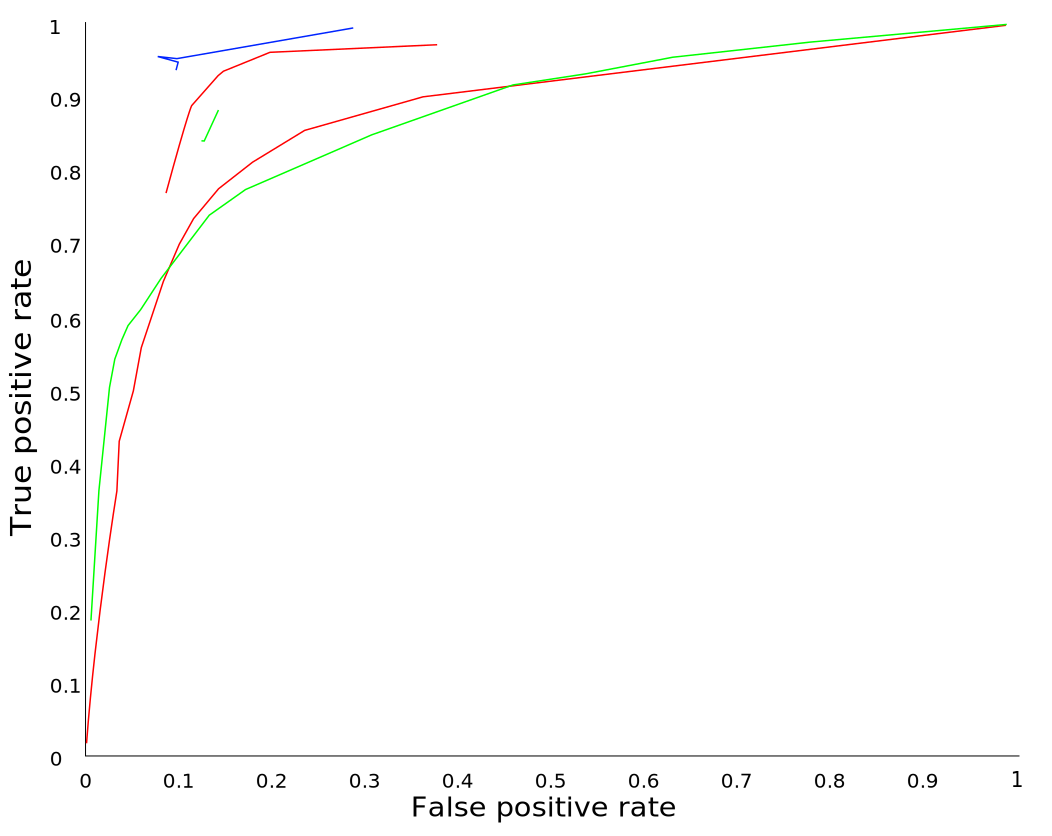
\includegraphics[width=1.0\textwidth]{images/graph.png}
\vskip -20px
%
\caption{\small ROC curves.
%
The lower green and red curves constitute the ROC for the log-end and
log-segment detectors respectively with varying thresholds~$t$ without the
grammar.
%
The upper green curve measures ROC for~$Z^+_q$ and~$Z^-_q$ under constraints
\ref{constraintA}--\ref{constraintE} varying the mapping from evidence to
priors.
%
The upper red curve measures ROC for~$Z^u_q$, $Z^v_q$, and~$Z^w_q$ under
constraints \ref{constraintA}--\ref{constraintD} and
\ref{constraintF}--\ref{constraintG} varying the mapping from evidence to
priors.
%
The blue curve measures ROC for~$Z^+_q$, $Z^-_q$, $Z^u_q$, $Z^v_q$, and~$Z^w_q$
under all constraints varying the mapping from evidence to priors.}
%
\label{fig-ll1:roc}
\vskip-3ex
\end{figure}

\begin{figure}
\centering
% \begin{tabular}{@{}c@{\hspace*{2pt}}c@{\hspace*{2pt}}c@{\hspace*{2pt}}c@{}}
% \includegraphics[width=0.25\textwidth]{images/1263244624-1500-matlab.jpeg}&
% \includegraphics[width=0.25\textwidth]{images/1263244624-1500-pb.jpeg}&
% \includegraphics[width=0.25\textwidth]{images/1263244624-1500-ncuts.jpeg}&
% \includegraphics[width=0.25\textwidth]{images/1263244624-1500-mshift.jpeg}\\
% (a)&(b)&(c)&(d)
% \end{tabular}
\begin{tabular}{@{}c@{\hspace*{2pt}}c@{}}
\includegraphics[height=0.215\textheight]{images/1263244624-1500-matlab.jpeg}&
\includegraphics[height=0.215\textheight]{images/1263244624-1500-pb.jpeg}\\
(a)&(b)\\[1ex]
\includegraphics[height=0.215\textheight]{images/1263244624-1500-ncuts.jpeg}&
\includegraphics[height=0.215\textheight]{images/1263244624-1500-mshift.jpeg}\\
(c)&(d)
\end{tabular}
\vspace*{-4ex}
\caption{\small A comparison with a number of standard edge detectors and segmentation methods.
%
Neither (a)~\Matlab's Canny edge detector nor (b)~the \Pb\ edge detector reliably find edges separating adjacent logs or log ends.
%
Neither (c)~Normalized Cut nor (d)~Mean Shift segment out the log parts.}
%
\label{fig-ll1:comparison}
\end{figure}


\begin{figure}
\centering
\begin{tabular}{@{}c@{\hspace*{2pt}}c@{\hspace*{2pt}}c@{\hspace*{2pt}}c@{\hspace*{2pt}}c@{}}
\includegraphics[width=0.195\textwidth]{images/1263244624-1500-0-raw.jpg}&
\includegraphics[width=0.195\textwidth]{images/1263244624-1500-0-segment.jpg}&
\includegraphics[width=0.195\textwidth]{images/1263244624-1500-0-end.jpg}&
\includegraphics[width=0.195\textwidth]{images/1263244624-1500-0-both.jpg}&
\includegraphics[width=0.195\textwidth]{images/1263244624-1500-0.jpg}\\[-0.7ex]
\includegraphics[width=0.195\textwidth]{images/1263244065-1200-ll-raw.jpg}&
\includegraphics[width=0.195\textwidth]{images/1263244065-1200-ll-segment.jpg}&
\includegraphics[width=0.195\textwidth]{images/1263244065-1200-ll-end.jpg}&
\includegraphics[width=0.195\textwidth]{images/1263244065-1200-ll-both.jpg}&
\includegraphics[width=0.195\textwidth]{images/1263244065-1200-ll.jpg}\\[-0.7ex]
\includegraphics[width=0.195\textwidth]{images/1263242135-1800-ll-raw.jpg}&
\includegraphics[width=0.195\textwidth]{images/1263242135-1800-ll-segment.jpg}&
\includegraphics[width=0.195\textwidth]{images/1263242135-1800-ll-end.jpg}&
\includegraphics[width=0.195\textwidth]{images/1263242135-1800-ll-both.jpg}&
\includegraphics[width=0.195\textwidth]{images/1263242135-1800-ll.jpg}\\[-0.7ex]
\includegraphics[width=0.195\textwidth]{images/1263242360-1800-0-raw.jpg}&
\includegraphics[width=0.195\textwidth]{images/1263242360-1800-0-segment.jpg}&
\includegraphics[width=0.195\textwidth]{images/1263242360-1800-0-end.jpg}&
\includegraphics[width=0.195\textwidth]{images/1263242360-1800-0-both.jpg}&
\includegraphics[width=0.195\textwidth]{images/1263242360-1800-0.jpg}\\[-0.7ex]
\includegraphics[width=0.195\textwidth]{images/1263243842-900-0-raw.jpg}&
\includegraphics[width=0.195\textwidth]{images/1263243842-900-0-segment.jpg}&
\includegraphics[width=0.195\textwidth]{images/1263243842-900-0-end.jpg}&
\includegraphics[width=0.195\textwidth]{images/1263243842-900-0-both.jpg}&
\includegraphics[width=0.195\textwidth]{images/1263243842-900-0.jpg}\\
(a)&(b)&(c)&(d)&(e)
\end{tabular}
%
\caption{\small (a)~Raw detector response.
%
(b)~Detector response with just constraints
  \ref{constraintA}--\ref{constraintD} and
  \ref{constraintF}--\ref{constraintG}.
%
(c)~Detector response with just constraints
  \ref{constraintA}--\ref{constraintE}.
%
(d)~Detector response with all constraints.
%
(e)~Estimated structure.
%
In~(a--d), bright red indicates true negative, dark red indicates false
negative, bright green indicates true positive, dark green indicates false
positive, and blue indicates occlusion.
%
In~(e), green indicates true positive and red indicates false negative.
%
There are no false positives and true negatives are not indicated.
%
We suggest that the reader view this figure at a high magnification level in a
PDF viewer to appreciate the images.
}
%
\label{fig-ll1:results}
\end{figure}

We took images of~32 distinct \LincolnLog\ structures, each from~5 distinct
poses resulting in a total of~160 images.
%
We performed foreground-background separation and pose estimation for all~160
images using the methods from section~\ref{sec-ll1:pose}.
%
Pose was estimated within~5mm translation and~2$^{\circ}$ rotation of ground
truth for~142 images.
%
We discarded the~18 images with inaccurate pose estimation and performed
structure estimation on the remainder.
%
The results for~5 images, all of distinct structures, are shown in
Fig.~\ref{fig-ll1:results}.
%
Fig.~\ref{fig-ll1:results}(a) was derived by thresholding the priors on~$Z^+_q$,
$Z^-_q$, $Z^u_q$, $Z^v_q$, and~$Z^w_q$ at $t=0.5$.
%
Fig.~\ref{fig-ll1:results}(b--d) were derived by solving a stochastic CSP with
various subsets of the constraints and rendering the values of~$Z^+_q$,
$Z^-_q$, $Z^u_q$, $Z^v_q$, and~$Z^w_q$ for the solution provided by the first
method in section~\ref{sec-ll1:structure}.
%
Fig.~\ref{fig-ll1:results}(e) was derived by solving the stochastic CSP with all
constraints and rendering the values of~$Z_q$ for the solution provided by the
first method in section~\ref{sec-ll1:structure}.
%
Note that our method determines the correct component type ($Z_q$) of most
occluded logs in the assemblies in the second row of Fig.~\ref{fig-ll1:results}(e).
%
It gives an incorrect component type for only a single log in that row.

We conducted experiments to determine how much the grammar improves the
accuracy of structure estimation.
%
We performed variants of the runs in Fig.~\ref{fig-ll1:results}(a-d), varying the
threshold~$t$ and the mapping from evidence to priors to produce the ROC curves
depicted in Fig.~\ref{fig-ll1:roc}.
%
The mapping function is varied through the weighting factor~$e$ for the linear
interpolator discussed in section~\ref{sec-ll1:mapping}.

Pose and structure estimation is sufficiently robust to support robotic
manipulation.
%
Supplementary material included on the website for this paper contains videos
of fully autonomous robotic disassembly of six different \LincolnLog\
structures whose pose and structure have been determined from a single image as
well as videos of semiautonomous robotic assembly of replicate \LincolnLog\
structures from the same estimated pose and structure.

\section{Conclusion}
\label{sec-ll1:conclusion}

\LincolnLogs\ are children's toys yet the computational problem we present is
\emph{not} a toy.
%
Pose and structure estimation of \LincolnLog\ assemblies is \emph{far} more
difficult than may appear on the surface.
%
The space of objects to be recognized is combinatorially large.
%
Much of every structure is in self occlusion.
%
The low contrast due to shadows and color, intensity, and texture uniformity
make it impossible to recognize even \emph{visible} logs with existing
techniques.
%
No standard edge detector (\eg\ Canny \cite{Canny1986} or \Pb\
\cite{Maire2008}) can reliably find edges separating adjacent logs or circular
log ends and no standard segmentation method (\eg\ Normalized Cut
\cite{Shi2000} or Mean Shift \cite{Comaniciu2002}) can reliably find log parts
\emph{even when fully visible} as shown in Fig.~\ref{fig-ll1:comparison}.
%
Even our filter-based feature detectors, which use pose information along with
constraints from the language model to \emph{tune to the expected feature at
  the expected image position}, produce correct binary decisions only about
65\% of the time.
%
Occlusion only makes matters worse.
%
Performing non-stochastic constraint satisfaction (\eg\ Waltz line labeling
\cite{Waltz1975}) on the binary output of these detectors leads to
inconsistent CSPs on \emph{all} images in our dataset.

We have demonstrated a visual domain that is generative in much the same way
that human language is generative.
%
We have presented a visual language model that improves recognition accuracy in
this domain in much the same way that language models improve
speech-recognition accuracy.
%
Unlike context-free models of human language, our visual language models are
context sensitive and formulated as stochastic CSPs.
%
Much of our visual experience in the artifactual world is perceiving generative
man-made structures like buildings, furniture, vehicles, \etc{}
%
Our \LincolnLog\ domain is a first step towards building visual language models
for such real-world domains.

Language models for vision are more complex than those for human language as
they must deal with occlusion resulting from perspective projection and pose
variation.
%
However, visual domains exhibit a novel possibility: recovering structure
despite occlusion by integrating the perceptual evidence from multiple images
of the same object taken from different poses.
%
In the \LincolnLog\ domain, one can carry this even further.
%
When faced with ambiguity arising from occlusion, a robot can partially
disassemble a structure to view occluded substructure and integrate perceptual
evidence from multiple images taken at different disassembly stages to yield a
complete unambiguous estimate of the structure of the original assembly prior
to disassembly.
%
Moreover, it is possible to integrate information about pose or structure from
different modalities.
%
One can integrate partial pose and structure information from one or more
images with partial pose and structure information expressed in human language
to yield a complete unambiguous estimate of pose and structure.
%
We are, in fact, able to do this and expect to report on this in the future.

\chapter{Seeing Unseeability to See the Unseeable}

\section{Introduction}
\label{sec:introduction}

\begin{quote}
  [T]here are known knowns; there are things we know we know.
  %
  We also know there are known unknowns; that is to say we know there are some
  things we do not know.
  %
  But there are also unknown unknowns --- the ones we don't know we don't know.
  \par\vspace*{-3ex}
  \begin{flushright}
    Donald Rumsfeld (12 February 2002)
  \end{flushright}
  \par\vspace*{-4ex}
\end{quote}

\noindent People exhibit the uncanny ability to see the unseeable.
%
The colloquial exhortation \emph{You have eyes in the back of your
  head!}\ expresses the assessment that someone is making correct judgments as
if they could see what is behind them, but obviously cannot.
%
People regularly determine the properties of occluded portions of objects from
observations of visible portions of those objects using general world knowledge
about the consistency of object properties.
%
Psychologists have demonstrated that the world knowledge that can influence
perception can be high level, abstract, and symbolic, and not just related to
low-level image properties such as object class, shape, color, motion, and
texture.
%
For example, \singleemcite{FreydPC88} showed that physical forces, such as
gravity, and whether such forces are in equilibrium, due to support and
attachment relations, influences visual perception of object location in adults.
%
\singleemcite{Baillargeon86,Baillargeon87} showed that knowledge of
substantiality, the fact that solid objects cannot interpenetrate, influences
visual object perception in young infants.
% Phil Kellman, Kestenbaum, Frank Keil, Larry Macomber, or ...someone in UMich
\singleemcite{Streri1988} showed that knowledge about object rigidity
influences both visual and haptic perception of those objects in young infants.
%
Moreover, such influence is cross modal: observable haptic perception
influences visual perception of unobservable properties and observable visual
perception influences haptic perception of unobservable properties.
% Karen Wynn UArizona
\singleemcite{Wynn1998} showed that material properties of objects, such as
whether they are countable or mass substances, along with abstract properties,
such as the number of countable objects and the quantity of mass substances, and
how they are transferred between containers, influences visual perception in
young infants.
%
Similar results exist for many physical properties such as relative mass,
momentum, etc.
%
These results demonstrate that people can easily integrate information from
multiple sources together with world knowledge to see the unseeable.

People so regularly invoke the ability to see the unseeable that we often don't
realize that we do so.
%
If you observe a person entering the front door of a house and later see them
appear from behind the house without seeing them exit, you easily see the
unseeable and conclude that there must be an unseen door to the house.
%
But if one later opens a curtain covering a large living-room bay window in the
front of the house so that you see through the house and see the back door you
no longer need to invoke the ability to see the unseeable.
%
A more subtle question then arises: when must you invoke the ability to see the
unseeable?
%
In other words how can you see unseeability, the inability to see?
%
This question becomes particularly thorny since, as we will see, it can
involve a chicken-and-egg problem: seeing the unseen can require seeing the
unseeability of the unseen and seeing the unseeability of the unseen can
require seeing the unseen.

The ability to see unseeability and to see the unseeable can further
dramatically influence human behavior.
%
We regularly and unconsciously move our heads and use our hands to open
containers to render seeable what was previously unseeable.
%
To realize that we need to do so in the first place, we must first see the
unseeability of what we can't see.
%
Then we must determine how to best use our perceptual, motor, and reasoning
affordances to remedy the perceptual deficiency.

We present a general computational framework for seeing unseeability to see the
unseeable.
%
We formulate and evaluate a particular instantiation of this general framework
in the context of a restricted domain, namely \LincolnLogs, a children's
assembly toy where one constructs assemblies from a small inventory of logs.
%
Two relevant aspects of this domain facilitate its use for investigating our
general computational framework: (a)~\LincolnLog\ assemblies suffer from
massive occlusion and (b)~a simple but rich expression of world knowledge, in
the form of constraints on valid assemblies, can mitigate the effects of such
occlusion.
%
While \LincolnLogs\ are a children's toy, this domain is far from a toy when it
comes to computer vision.
%
The task of structure estimation, determining, from an image, the correct
combination of component logs used to construct an assembly and how they are
combined, is well beyond the state of the art.
%
Not only is the computer-vision problem for this domain immensely
difficult---occlusion, luminance variation, and a distinct paucity of features
all encumber the process---the computational problem itself affords a richness
and complexity that is not readily apparent.

We present methods for seeing the unseeable (in Section~\ref{sec:structure})
and seeing unseeability (in Section~\ref{sec:visibility}) based on precise
computation of the maximum-likelihood structure estimate.
%
Section~\ref{sec:confidence} presents a rational basis for determining
confidence in one's structure estimate despite unseeability based on precise
computation of the amount of evidence needed to override a uniform prior on the
unseeable.
%
Section~\ref{sec:integration} presents an active-vision decision-making
process for determining rational behavior in the presence of unseeability based
on precise computation of which of several available perception-enhancing
actions one should take to maximally improve the confidence in one's structure
estimate.
%
Such capability is bootstrapped by our framework's capacity to integrate
evidence from different views, both \emph{imagined} and \emph{actual}.
%
Section~\ref{sec:language} further highlights the elegance of our framework by
demonstrating the integration of evidence \emph{across} modalities; using
natural-language descriptions to aid in resolving ambiguities in structure
estimation.

\par\vspace{-1ex}
\section{Structure Estimation}
\label{sec:structure}

Speech recognizers use a human language model, on utterances in a generative
linguistic domain, to improve recognition accuracy over the raw recognition
rate of the phoneme detectors.
%
Analogously, \singleemcite{Siddharth2011} use a visual language
model, on compositional visual structures in a generative visual domain, to
improve recognition accuracy over the raw recognition rate of the part
detectors.
%
In this approach, a complex object is constructed out of a collection of parts
taken from a small part inventory.
%
A language model, in the form of a stochastic constraint-satisfaction problem
(CSP; \npcite{Lauriere1978}), characterizes the constrained way object parts can
combine to yield a whole object and significantly improves the recognition rate
of the whole structure over the infinitesimally small recognition rate that
would result from unconstrained application of the unreliable part detectors.
%
Unlike the speech-recognition domain, where (except for coarticulation) there
is acoustic evidence for all phonemes, in the visual domain there may be
components with no image evidence due to occlusion.
%
A novel aspect of applying a language model in the visual domain instead of the
linguistic domain is that it can additionally help in recovering occluded
information.

\begin{figure}
  \centering
  \begin{tabular}{@{}c@{\hspace{2pt}}c@{}}
    \includegraphics[width=0.47\textwidth]{images/real-log-qw}&
    \includegraphics[width=0.493\textwidth]{images/pose2-cut}\\
    (a)&(c)
  \end{tabular}
  \vspace*{2ex}
  \begin{tabular}{@{}c@{\hspace{2pt}}c@{\hspace{2pt}}c@{\hspace{2pt}}c@{}}
    \includegraphics[width=0.24\textwidth]{images/poss-0-small}&
    \includegraphics[width=0.24\textwidth]{images/poss-1-small}&
    \includegraphics[width=0.24\textwidth]{images/poss-2-small}&
    \includegraphics[width=0.24\textwidth]{images/poss-3-small}\\
    $\emptyset$&$(1,1)$&$(1,2)$&$(2,2)$\\[1ex]
    \includegraphics[width=0.24\textwidth]{images/poss-4-small}&
    \includegraphics[width=0.24\textwidth]{images/poss-5-small}&
    \includegraphics[width=0.24\textwidth]{images/poss-6-small}&\\
    $(1,3)$&$(2,3)$&$(3,3)$&\\
    \multicolumn{4}{c}{(b)}
  \end{tabular}
  %
  \par\vspace*{-2ex}
  %
  \caption{We generate two kinds of random variables for each grid
    position~$q$: log-feature variables~(a) that encode the observed image
    evidence for portions of logs and log-occupancy variables~(b) that encode
    the structure.
    %
    The overall process of structure estimation involves determining the
    unknown values of the log-occupancy variables~(b) from the observed image
    evidence represented through provided values of the log-feature
    variables~(a).
    %
    This process is mediated through the constraints shown in
    Figure~\protect\ref{fig:grammar-assemblies}(a).
    %
    (a)~The Boolean log-feature variables~$Z^+_q$, $Z^-_q$, $Z^u_q$, $Z^v_q$,
    and~$Z^w_q$ encode the presence of the specified image features for grid
    position~$q$.
    %
    (b)~The log-occupancy variable~$Z_q$ for grid position~$q$ takes one of
    a finite set of possible values: $\emptyset$~to denote that~$q$ is
    unoccupied and $(m,n)$ to denote occupancy by the~$m^{\textrm{th}}$ notch
    of an $n$-notch log.
    %
    (c)~Example of the underlying symbolic grid of a \LincolnLog\
    assembly.}
  %
  \label{fig:lincoln-logs}
  \par\vspace*{-2.5ex}
\end{figure}

This approach is demonstrated in the domain of \LincolnLogs, a children's
assembly toy with a small part inventory, namely, 1-, 2-, and 3-notch
logs.
%
In a grammatical \LincolnLog\ assembly, all logs lie on a symbolic grid imposed
over the structure (Figure~\ref{fig:lincoln-logs}c).
%
The structure of an assembly can be completely and unambiguously described by
specifying the occupancy at each grid position
(Figure~\ref{fig:lincoln-logs}b).
%
Not all possible occupancy descriptions denote stable, physically realizable
structures.
%
The space of valid structures can be specified by local constraints on the
occupancy of adjacent grid positions, as shown in
Figure~\ref{fig:grammar-assemblies}(a).
%
Enforcing these constraints over the entire structure renders some assemblies
grammatical and others ungrammatical, as shown in
Figure~\ref{fig:grammar-assemblies}(b).

\begin{figure}
  \centering
  \begin{tabular}{@{}l@{}}
    2-notch logs occupy 2 adjacent grid points\\
    3-notch logs occupy 3 adjacent grid points\\
    1- and 2-notch logs must be supported at all notches\\
    3-notch logs must be supported in at least 2 notches\\
    log ends must be at the ends of logs\\
    short segments indicate occupancy above or below\\
    long segments indicate presence of a multi-notch log\\[1ex]
    \multicolumn{1}{c}{(a)}
  \end{tabular}
  \par\vspace*{2ex}
  \begin{tabular}{@{}c@{\hspace{2pt}}c@{}}
    \includegraphics[width=0.48\textwidth]{images/valid-assemblies-1}&
    \includegraphics[width=0.48\textwidth]{images/valid-assemblies-2}\\[-0.5ex]
    \includegraphics[width=0.48\textwidth]{images/invalid-assemblies-1}&
    \includegraphics[width=0.48\textwidth]{images/invalid-assemblies-2}\\[1ex]
    \multicolumn{2}{c}{(b)}
  \end{tabular}
  %
  \par\vspace*{-2ex}
  %
  \caption{(a)~The constraints that encode the grammar of \LincolnLogs.
    %
    (b, top)~Examples of structures that satisfy the grammar.
    %
    (b, bottom)~Examples of structures that do not satisfy the grammar, because
    of unsupported logs.}
  %
  \label{fig:grammar-assemblies}
  %
  \par\vspace*{-3ex}
\end{figure}

\LincolnLogs, being cylindrical, generate two predominant image features:
\defoccur{log ends}, ellipses that result from the perspective projection of
circular log ends, and \defoccur{log segments}, line segments that result from
the perspective projection of cylindrical walls.
%
Boolean random variables~$Z^+$ and~$Z^-$ are constructed to encode the
presence of log-end features in the image.
%
Similar Boolean random variables~$Z^u$, $Z^v$, and~$Z^w$ are constructed
to encode the presence of log-segment features in the image.
%
There is one instance of each such variable, $Z^+_q$, $Z^-_q$, $Z^u_q$,
$Z^v_q$, and~$Z^w_q$, for each grid position~$q$, as shown in
Figure~\ref{fig:lincoln-logs}(a).
%
We also construct a discrete random variable~$Z_q$ for each grid position~$q$
that ranges over its possible occupancies in the structure, as shown in
Figure~\ref{fig:lincoln-logs}(b).
%
In the exposition below, we use~$\mathbf{Z}^+$, $\mathbf{Z}^-$, $\mathbf{Z}^u$,
$\mathbf{Z}^v$, $\mathbf{Z}^w$, and~$\mathbf{Z}$ to denote the collections of
the variables~$Z^+_q$, $Z^-_q$, $Z^u_q$, $Z^v_q$, $Z^w_q$, and~$Z_q$ for all
of the grid positions~$q$ in the problem at hand.

The values of the log-feature variables are determined directly from the image.
%
The values of the log-occupancy variables, however, cannot be directly observed.
%
The essence of structure estimation is to determine the values of the
log-occupancy variables.
%
This is done by formulating and solving a constraint satisfaction problem that
mutually constraints the log-feature and log-occupancy variables, using
Algorithm~\ref{alg:structure}.
%
The constraints are formalizations of the world knowledge in
Figure~\ref{fig:grammar-assemblies}(a).
%
Because the image evidence as encoded in the log-feature variables is noisy,
unreliable, and incomplete (due to occlusion), we cannot treat this as a
symbolic CSP and instead treat this as a stochastic CSP.
%
Within this stochastic framework, structure estimation is performed by
establishing priors over the random variables~$Z^+_q$, $Z^-_q$, $Z^u_q$,
$Z^v_q$, and~$Z^w_q$ that correspond to log features using image evidence and
establishing a uniform prior over the random variables~$Z_q$ that correspond to
the latent structure.
%
The random variables that correspond to log features are marginalized
\footnote{Marginalization is the process of deriving the joint distribution~$M$
  of a \emph{subset}, say~$\{A\}$, of the constituent variables of a joint
  distribution over all of the variables, say $\{A,B,C\}$.
  %
  We compute such as $M = \Pr\left(A\right) = \sum_{B,C} \Pr\left(A,B,C\right)$.
  %
  We utilize this in order to be able to derive the distribution over log
  occupancies, which is what we want, from the joint distribution over
  log occupancies and observed image evidence, which is what we have.
  %
  Historically, this term evolved from the practice of displaying the values of
  a joint distribution $\Pr(A,B)$ as a two-dimensional table with rows for
  the~$A$ entries and columns for the~$B$ entries.
  %
  The values of $\Pr(A)$ were derived by summing along the columns to yield a
  new row at the bottom \emph{margin} of the table.
  %
  The values of $\Pr(B)$ were derived by summing along the rows to yield a
  new column at the right \emph{margin} of the table.
  %
  This led to $\Pr(A)$ and $\Pr(B)$ being referred to as \emph{marginal}
  probabilities and the derivation process as \emph{marginalization}.}
and the resulting marginal distribution is conditioned on the language
model~$\Phi$ to enforce the constraints from
Figure~\ref{fig:grammar-assemblies}(a).
%
Finally, the assignment to the collection, $\mathbf{Z}$, of random
variables~$Z_q$, that maximizes this conditional marginal probability is
computed:

\par\vspace*{-2ex}
\begin{equation}
  \argmax_{\mathbf{Z}}\hspace{-13pt}
  \sum_{\substack{\mathbf{Z}^+,\mathbf{Z}^-,\mathbf{Z}^u,\mathbf{Z}^v,\mathbf{Z}^w\\
      \Phi\left[\mathbf{Z},\mathbf{Z}^+,\mathbf{Z}^-,\mathbf{Z}^u,\mathbf{Z}^v,\mathbf{Z}^w\right]}}
  \hspace{-10pt}\Pr\left(\mathbf{Z},\mathbf{Z}^{+},\mathbf{Z}^{-},\mathbf{Z}^u,\mathbf{Z}^v,\mathbf{Z}^w\right)
  \label{eq:structure-estimation}
\end{equation}
%
While this method can determine the conditional probability distribution over
consistent structures given image evidence, doing so is combinatorially
intractable.
%
To see why this is so, consider a simple $2 \times 2 \times 2$ grid
representing the underlying structure of a hypothetical \LincolnLog\ assembly.
%
Even for so small an assembly, since each grid position can take one of seven
possible values, the total number of possibilities ($7^8 \approx 5 \times
10^6$), exponential in the number of grid points, is huge.
%
This is due to the generative nature of the \LincolnLog\ domain.
%
We illustrate this point further with Figure~\ref{fig:complexity}(c), where we
enumerate the number of possible structures and how many of such are valid
given our system of constraints, for a few relatively small grid sizes.

\begin{figure}
  \centering
  \begin{tabular}{@{}c@{\hspace*{2pt}}c@{}}
    \includegraphics[width=0.45\textwidth]{images/log-end-visibility}&
    \includegraphics[width=0.45\textwidth]{images/log-segment-visibility}\\
    (a)&(b)
  \end{tabular}
  \par\vspace*{1ex}
  \begin{tabular}{@{}rc@{}}
    \raisebox{15ex}{(c)}&
    \begin{tabular}[b]{@{}c@{\hspace{10pt}}r@{\hspace{10pt}}r@{\hspace{10pt}}r@{}}
      \toprule
      $\substack{\text{\normalsize size}\\[0.5ex]
        \left(\text{X} \times \text{YX} \times \text{YZ} \times \text{Z}\right)}$ &
      \# grid points &
      $\substack{\text{\normalsize possible}\\ \text{\normalsize structures}}$ &
      $\substack{\text{\normalsize valid}\\ \text{\normalsize structures}}$\\[1ex]
      \midrule
      $2 \times 2 \times 2 \times 2$ &           $8$ & $5 \times 10^{6}$ &    $233$\\
      $2 \times 3 \times 2 \times 2$ &          $12$ &         $10^{10}$ &   $1341$\\
      $2 \times 3 \times 3 \times 2$ &          $16$ &         $10^{13}$ &   $6667$\\
      $3 \times 2 \times 2 \times 3$ &          $12$ &         $10^{10}$ &   $5461$\\
      $3 \times 2 \times 2 \times 3$ &          $18$ &         $10^{15}$ & $670179$\\
      \bottomrule
    \end{tabular}\\
    \raisebox{15ex}{(d)} & \includegraphics[width=0.55\textwidth]{images/robots}
  \end{tabular}
  %
  \par\vspace*{-2ex}
  %
  \caption{Example visibility estimates for (a)~log ends and (b)~log segments.
    %
    Green and orange indicate the visible and occluded features for
    even layers, while blue and magenta indicate visible and occluded features
    for odd layers.
    %
    (c)~Size of the space of \LincolnLog\ assemblies for given grid
    sizes.
    %
    $XZ$~is the ground plane while~$YX$ and~$YZ$ are the heights of the
    assembly along the respective ground-plane axes.
    %
    (d)~Our robotic environment for performing structure estimation
    with a rotating head to image the assembly from different viewpoints and a
    robot arm to disassemble the assembly.}
  %
  \label{fig:complexity}
  %
  \par\vspace*{-5ex}
\end{figure}

\begin{algorithm}[t]
  \caption{The structure-estimation algorithm as described in
    Section~\ref{sec:structure}.}
  %
  \SetKwData{Feature}{log-feature}
  \SetKwData{Features}{log-features}
  \SetKwData{GridPositions}{grid-positions}
  \SetKwData{GridPosition}{grid-position}
  \SetKwData{Grid}{grid}
  \SetKwData{BestP}{best-probability}
  \SetKwData{BestS}{best-structure}
  \SetKwData{Pro}{probability}
  \SetKwData{Image}{image}
  \SetKwData{Constraints}{constraints}
  \SetKwFunction{Uniform}{uniform}
  \SetKwFunction{Detector}{detector}
  \SetKwFunction{Nonempty}{nonempty}
  \SetKwFunction{Bound}{bound}
  \SetKwFunction{Probability}{Pr}
  \SetKwFunction{Backtrack}{backtrack}
  \SetKwFunction{Bind}{bind}
  \SetKwFunction{Unbound}{unbound}
  \SetKwFunction{Bound}{bound}
  \SetKwFunction{Select}{select}
  \SetKwFunction{AC}{arc-consistency}
  \SetKwFunction{CSPSolutionsExist}{csp-solutions-exist}
  \SetKwFunction{Inconsistent}{inconsistent}
  \GridPositions$\leftarrow$ $(\forall_{\GridPosition\in\Grid})$
  \Uniform{$\{\emptyset,(1,1),(1,2),(2,2),(1,3),(2,3),(3,3)\}$}\;
  \Features$\leftarrow$ $(\forall_{\Feature\in\Grid})$
  \Detector{\Feature,\Image}\;
  \BestP$\leftarrow-\infty$\;
  \While{\CSPSolutionsExist{}}{
    \Pro$\leftarrow$\hspace{-5ex}$\displaystyle \prod_{\Bound{\Features}}$\hspace{-5ex}
    \Probability{\Feature}\hspace{-5ex}$\displaystyle
    \prod_{\Bound{\GridPositions}}$ \hspace{-5ex}\Probability{\GridPosition}\;
    \If{$(\forall_{\Features})$\Bound{\Feature}$\wedge$
      $(\forall_{\GridPositions})$\Bound{\GridPosition}}{
      \If{\Pro$>$ \BestP}{\BestP$\leftarrow$ \Pro\;
        \BestS$\leftarrow$ \GridPositions\;
      }
      \Backtrack{}\;
    }
    \lIf{\Pro$<$ \BestP}{\Backtrack{}}\;
    \Bind{\Select{\Unbound{\GridPosition$\cup$ \Feature}}}\;
    \AC{\Constraints}\;
    \lIf{\Inconsistent{}}{\Backtrack{}}
  }
  \label{alg:structure}
\end{algorithm}

To compute Equation~\ref{eq:structure-estimation}, we employ algorithms
for each of the constituent processes that help ameliorate this intractability.
%
These algorithms prune the space so as not to enumerate all possible
structures, and hence cannot obtain the distribution over structures.
%
The conditional marginalization process is made tractable by pruning
assignments to the random variables that violate the grammar~$\Phi$ using arc
consistency \cite{Mackworth1977}.
%
The maximization process is made tractable by using a branch-and-bound
algorithm \cite{Land1960} that maintains upper and lower bounds on the maximal
conditional marginal probability.
%
Instead of determining the distribution over structures, this yields a single
most-likely consistent structure given the image evidence, along with its
probability.
%
Algorithm~\ref{alg:structure} gives pseudo-code for the structure-estimation
process.

\par\vspace{-1ex}
\section{Visibility Estimation}
\label{sec:visibility}

Image evidence for the presence or absence of each log feature is obtained
independently.
%
Each log feature corresponds to a unique local image property when projected to
the image plane under the known camera-relative pose.
%
A prior over the random variable associated with a specific log feature can be
determined with a detector that is focused on the expected location and shape
of that feature in the image given the projection.
%
This assumes that the specific log feature is visible in the image, and not
occluded by portions of the assembly between the camera and that log feature.
%
We show example visibility of log-end and log-segment features for a simple
\LincolnLog\ assembly in Figure~\ref{fig:complexity}(a,b).
%
When the log feature~$f$, a member of the set $\{+,-,u,v,w\}$ of the five
feature classes defined above, at a position~$q$, is not visible, the prior can
be taken as uniform, allowing the grammar to fill in unknown information.
%
We represent the visibility of a feature~$f$ at position~$q$ by the boolean
variable~$V^f_q$, where:

\par\vspace*{-4ex}
\begin{subequations}
  \begin{align}
    &\Pr(Z^f_q=\true)\propto\text{image evidence}&\text{when $V^f_q=\true$}\\[-1ex]
    &\Pr(Z^f_q=\false)=\frac{1}{2}&\text{otherwise.}
  \end{align}
  \label{eq:visibility}
  \vspace*{-2ex}
\end{subequations}

\par\vspace*{-1ex}\noindent
In order to do so, it is necessary to know which log features are visible and
which are occluded so that image evidence is only applied to construct a prior
on visible log features, using Equation~\ref{eq:visibility}(a), and a uniform
prior is constructed for occluded log features, using
Equation~\ref{eq:visibility}(b).
%
Thus, in Rumsfeld's terminology, one needs to know the known unknowns in order
to determine the unknowns.
%
This creates a chicken-and-egg problem.
%
To determine whether a particular log feature is visible, one must know the
composition of the structure between that feature and the camera.
%
Likewise, to determine the structure composition, one must know which log
features are visible.
%
While earlier work \cite{Siddharth2011} demonstrated successful automatic
determination of log occupancy at occluded log positions, it could only do so
given manual annotation of log-feature visibility.
%
In other words, while~$Z_q$ was automatically inferred, it required manual
annotation of~$V^f_q$.
%
Further, manual annotation of~$V^f_q$ required implicit human awareness
of~$Z_q$.

We extend this prior work to automatically determine visibility of log features
in tandem with log occupancy.
%
Our novel contribution in this section is mutual automatic determination of
both~$Z_q$ and~$V^f_q$ solving the chicken-and-egg problem inherent in doing so
with an iterative algorithm reminiscent of expectation maximization
\cite{DempsterLR77}.
%
We start with an initial estimate of the visibility of each log feature.
%
We apply the structure-estimation procedure to estimate the occupancy of each
symbolic grid position and use the estimated structure to recompute a new
estimate of log-feature visibility and iterate this process until a fixpoint is
reached.
%
There are two crucial components in this process: determining the initial
log-feature visibility estimate and reestimating log-feature visibility from an
estimate of structure.

We determine the initial log-feature visibility estimate, $V^f_q$, by assuming
that the structure is a rectangular prism whose top face and two camera-facing
front faces are completely visible, and whose other faces are not.
%
No assumptions are made about the constituents of the structure, its pose, or
the camera views used.
%
We use the camera-relative pose of the symbolic grid (which can be determined
without any knowledge of the structure) together with the maximal extent of
each of the three symbolic grid axes, three small integers which are currently
specified manually, to determine the visible faces.
%
We determine the image positions for four corners of the base of this
rectangular prism and the bottommost three such image positions as they
correspond to the endpoints of the lower edges of the two frontal faces.
%
It is possible that one of these faces is nearly parallel to the
camera axis and thus invisible.
%
We determine that this is the case when the angle subtended by the two lower
edges is less than 110$^{\circ}$ and discard the face whose lower edge has
minimal image width.
%
This process does nothing more than establish that, in the absence of a
structure estimate from which to derive visibility, the front and top faces of
the grid are the only parts for which the log-feature random variables have
image evidence as their support, using Equation~\ref{eq:visibility}(a).
%
All other parts of the grid are taken to have the uniform distribution as their
support, using Equation~\ref{eq:visibility}(b), as a means of saying that we
assume nothing about them.

We update the log-feature visibility estimate from a structure estimate by
rendering the structure in the context of the known camera-relative pose of the
symbolic grid.
%
We characterize each log feature with a fixed number of points, equally spaced
around circular log ends or along linear log segments and trace a ray from each
such point's 3D position to the camera center, asking whether that ray
intersects some bounding cylinder for a log in the estimated structure.
%
We take a log feature to be occluded when 60\% or more of such rays intersect
logs in the estimated structure.
%
Structure estimation isn't adversely affected by a moderate number of log
features incorrectly labeled as occluded because it can use the grammar to
determine occupancy of the corresponding grid positions.

\begin{algorithm}[t]
  \caption{The visibility-estimation algorithm as described in
    Section~\ref{sec:visibility}, using Algorithm~\ref{alg:structure}.}
  %
  \SetKwData{Feature}{log-feature}
  \SetKwData{Features}{log-features}
  \SetKwData{Visible}{visible}
  \SetKwData{Grid}{grid}
  \SetKwData{PreviousStructure}{previous-structure}
  \SetKwData{CurrentStructure}{current-structure}
  \SetKwData{RenderedImage}{rendered-image}
  \SetKwFunction{RenderStructure}{render-structure}
  \SetKwFunction{SE}{structure-estimation}
  \SetKwFunction{IsVisible}{is-visible}
  \Visible$\leftarrow$ \emph{top and front of structure}\;
  \CurrentStructure$\leftarrow$ $\emptyset$\;
  \Repeat{\PreviousStructure $=$ \CurrentStructure}{
    \PreviousStructure$\leftarrow$ \CurrentStructure\;
    \CurrentStructure$\leftarrow$ \SE{$(\forall_{\Feature \notin \Visible})\Pr(\Feature) = \frac{1}{2}$}\;
    \Visible$\leftarrow$ $\emptyset$\;
    \RenderedImage$\leftarrow$ \RenderStructure{\CurrentStructure}\;
    \ForAll{\Features$\in$ \Grid}{
      \lIf{\IsVisible{\Feature, \RenderedImage}}{\Visible $\leftarrow$
        \Visible $\cup$ $\{\Feature\}$
      }
    }
  }
  \label{alg:visbility}
\end{algorithm}

We perform such rendering efficiently by rasterization.
%
We begin with an empty bitmap, iterate over each log feature and each occupied
grid position that lies between that log feature and the camera center, and
render a projection of the bounding cylinder of the log at that grid position
on the bitmap.
%
This renders all possible occluders for each log feature, allowing one to
determine visibility by counting the rendered pixels at points that correspond
to the projected rays.

The above process might not reach a fixpoint and instead enter an infinite loop
of pairs of visibility and structure estimates.
%
In practice, this process reaches a fixpoint or enters a short loop within
three to four iterations, making loop detection straightforward.
%
When a loop is detected, we select the structure in the loop with the highest
probability estimate.
%
Algorithm~\ref{alg:visbility} provides the pseudo-code that summarizes the
above process.

\par\vspace{-1ex}
\section{Structure-Estimation Confidence}
\label{sec:confidence}

While the structure-estimation process can determine the occupancy of a small
number of grid positions when only a single set of occupancy values is
consistent with the grammar and the image evidence, it is not clairvoyant; it
cannot determine the structure of an assembly when a large part of that
assembly is occluded and many different possible structures are consistent with
the image evidence.
%
In this case, we again have an issue of unknowns \vs\ known unknowns: how can
one determine one's confidence in one's structure estimation?
%
If we could determine the conditional distribution over consistent structures
given image evidence, $\Pr(\mathbf{Z}|I)$, a measure of confidence could be
entropy of this distribution, $H(\mathbf{Z}|I)$.
%
However, as discussed previously, computing this distribution is intractable
and consequently so is computing its entropy.\footnote{The entropy $H(Z)$ of a
  random variable~$Z$ is $\sum_{z\in Z}\Pr(z)\log\Pr(z)$.
  %
  It measures the information content of a random variable, or lack thereof.
  %
  Computing this requires summing over all elements in~$Z$.}
%
Thus we adopt an alternate means of measuring confidence in the result of the
structure-estimation process.

Given a visibility estimate, $V^f_q$, structure estimate, $\mathbf{Z}$, and
priors on random variables associated with log features computed with
image evidence, $Z^f_q$, one can marginalize over the random variables
associated with visible log features and compute the maximum-likelihood
assignment to the random variables associated with occluded log features,
$\hat{\mathbf{Z}}^f$, consistent with a given structure estimate:
%
\begin{equation*}
  \hat{\mathbf{Z}}^f=
  \argmax_{\substack{Z^f_q\\V^f_q=\false}}\hspace{-4.5ex}
  \sum_{\substack{Z^f_q\\V^f_q=\true\\
      \Phi[\mathbf{Z},\mathbf{Z}^{+},\mathbf{Z}^{-},\mathbf{Z}^u,\mathbf{Z}^v,\mathbf{Z}^w]}}\hspace{-6ex}
  \Pr(\mathbf{Z},\mathbf{Z}^{+},\mathbf{Z}^{-},\mathbf{Z}^u,\mathbf{Z}^v,\mathbf{Z}^w)
\end{equation*}
%
One can then ask the following question: what is the maximal amount~$\delta$
that one can shift the probability mass on the occluded log-feature random
variables \emph{away} from the uniform prior, reassigning it to the opposite
element of its support, such that estimated structure remains the same?
%
Or in simpler terms: \emph{Assume an initial structure estimate derived from a
  uniform prior over occluded log features.
  %
  How much hypothetical evidence for such features is needed to change my mind
  about the structure?}
%
We compute~$\delta$ using a modified structure-estimation step:
%
\begin{equation*}
  \argmax_{\mathbf{Z}}\hspace{-5ex}
  \sum_{\substack{\mathbf{Z}^{+},\mathbf{Z}^{-},\mathbf{Z}^u,\mathbf{Z}^v,\mathbf{Z}^w\\
      \Phi[\mathbf{Z},\mathbf{Z}^{+},\mathbf{Z}^{-},\mathbf{Z}^u,\mathbf{Z}^v,\mathbf{Z}^w]}}\hspace{-5ex}
  \Pr(\mathbf{Z},\mathbf{Z}^{+},\mathbf{Z}^{-},\mathbf{Z}^u,\mathbf{Z}^v\,\mathbf{Z}^w)=\mathbf{Z}
\end{equation*}
%
when, for all $q^f$ where $V^f_q=\false$,
%
\begin{math}
    \Pr(Z^f_q=\neg\hat{Z}^f_q)=\frac{1}{2}+\delta
\end{math}
and
\begin{math}
    \Pr(Z^f_q=\hat{Z}^f_q)=\frac{1}{2}-\delta.
\end{math}
%
We call such a~$\delta$ the \defoccur{estimation tolerance}.
%
Then, for any estimated structure, one can make a confidence judgment by
comparing the estimation tolerance to an overall tolerance threshold~$\delta^*$.
%
One wishes to select a value for~$\delta^*$ that appropriately trades off false
positives and false negatives in such confidence judgments: we want to
minimize the cases that result in a positive confidence assessment for an
incorrect structure estimate and also minimize the cases that result in a
negative confidence assessment for a correct structure estimate.
%
Because the methods we present in the next section can gather additional
evidence in light of negative confidence assessment in structure estimation,
the former are more hazardous than the latter because they preclude gathering
additional evidence and lead to an incorrect structure estimate while the
latter simply incur the cost of additional evidence gathering.
%
Because of this asymmetry, our method is largely insensitive to the particular
value of~$\delta^*$ so long as it is sufficiently high to not yield excessive
false positives.

One can determine the estimation tolerance by binary search for the smallest
value of $\delta\in(0,0.5)$ that results in a different estimated structure, a
time-consuming process.
%
But we don't actually need the value of~$\delta$; we only need to determine
whether $\delta<\delta^*$.
%
We do this by simply asking whether the estimated structure, $\mathbf{Z}$,
changes when the probabilities are shifted by~$\delta^*$, \ie\
%
\begin{math}
    \Pr(Z^f_q=\neg\hat{Z}^f_q)=\frac{1}{2}+\delta^{*}
\end{math}
and
\begin{math}
    \Pr(Z^f_q=\hat{Z}^f_q)=\frac{1}{2}-\delta^{*}
\end{math}.
%
This involves only a single new structure estimation.
%
Initializing the branch-and-bound structure-estimation algorithm with the
probability of the original structure estimate given the modified distributions
for the random variables associated with occluded log features speeds this
process up.

\par\vspace{-1ex}
\section{Gathering Additional Evidence}
\label{sec:integration}

Structure estimation can be made more reliable by integrating multiple sources
of image evidence.
%
We perform structure estimation in a robotic environment, illustrated in
Figure~\ref{fig:complexity}(d), that facilities automatically gathering
multiple sources of image evidence as needed.
%
This workspace is imaged by a camera mounted on a pendulum arm that can rotate
180$^{\circ}$ about the workspace, under computer control, to image the
assembly from different viewpoints.
%
This can be used to view portions of the assembly that would otherwise be
occluded.
%
Moreover, a robotic arm can disassemble a structure on the workspace to reveal
the lower layers of a structure that would otherwise be occluded by higher
layers.
%
These methods can further be combined.
%
Generally speaking, we seek a method for constraining a single estimate
of an initial structure with multiple log features derived from different
viewpoints and different stages of disassembly.

We can do this as follows.
%
Let~$\mathbf{Z}$ be a collection of random variables~$Z_q$ associated with log
occupancy for a given initial structure.
%
Given multiple views $i=1,\ldots,n$ with collections~$\mathbf{Z}_i$ of random
variables~$Z^+_q$, $Z^-_q$, $Z^u_q$, $Z^v_q$, and~$Z^w_q$ associated with the
image evidence for log features from those views, we can compute:
%
\begin{equation*}
  \argmax_{\mathbf{Z}}\hspace{-12pt}
  \sum_{\substack{\mathbf{Z}_1\ldots\mathbf{Z}_n\\
      \Phi\left[\mathbf{Z},\mathbf{Z}_1\right]\wedge\cdots\wedge\Phi\left[\mathbf{Z},\mathbf{Z}_n\right]}}
  \hspace{-10pt}\Pr\left(\mathbf{Z},\mathbf{Z}_1,\ldots,\mathbf{Z}_n\right)
\end{equation*}
%
Two issues arise in doing this.
%
First, though one can estimate the camera-relative pose of the structure
independently for each view, this does not yield the registration between these
views.
%
There are only four possible symbolic orientations of the structure in each
view so for~$n$ views we need only consider~$4^{n-1}$ possible combinations.
%
We can greedily search for the combination that yields the maximum-likelihood
structure estimate by incrementally adding views to the structure-estimation
process and registering each added view by searching for the best among the
four possible registrations.
%
Second, in the case of partial disassembly, we need to handle the fact that the
partially disassembled structure is a proper subset of the initial structure.
%
We do this by omitting random variables associated with log features
for logs that are known to have been removed in the disassembly process and not
instantiating constraints that mention such omitted random variables.

We can combine the techniques from Section~\ref{sec:confidence} with these
techniques to yield an active-vision \cite{Bajcsy1988} approach to producing a
confident and correct structure estimate.
%
One can perform structure estimation on an initial image and assess one's
confidence in that estimate.
%
If one is not confident, one can plan a new observation, entailing either a new
viewpoint, a partial-disassembly operation, or a combination of the two and
repeat this process until one is sufficiently confident in the estimated
structure.
%
We plan new observations by asking the following question: which of the
available actions maximally increases confidence?
%
Like before, if we could determine the conditional distribution over consistent
structures given image evidence, we could select the action which maximally
decreases entropy.
%
But again, neither computing this distribution nor consequently computing its
entropy is tractable, as discussed previously.
%
Thus we adopt an alternate means of measuring increase in confidence.

Consider view~$i$ of the~$n$ current views.
%
For such~$i$, consider the given visibility estimates $V^f_{iq}$, priors
$Z^f_{iq}$ on the log-feature random variables computed with image evidence,
and a structure estimate~$\mathbf{Z}$ constructed from such views.
%
We can marginalize over random variables associated with visible log features
$V^f_{iq} = \true$ and compute the maximum-likelihood assignment
$\hat{\mathbf{Z}}^f$ to the random variables associated with occluded log
features that is consistent with a given structure estimate:
%
\begin{equation*}
  \hat{\mathbf{Z}}^f=\argmax_{\substack{Z^f_{iq},V^f_{iq}=\false}}
  \sum_{\substack{Z^f_{iq},V^f_{iq}=\true\\
      \Phi[\mathbf{Z},\mathbf{Z}_1]\wedge\cdots\wedge\Phi[\mathbf{Z},\mathbf{Z}_n]}}
  \Pr(\mathbf{Z},\mathbf{Z}_1,\ldots,\mathbf{Z}_n)
\end{equation*}
%
We determine those log features that are invisible in all current views but
visible in a new view resulting from a hypothetical action.
%
One can then ask the following question: what is the maximal amount~$\delta'$
that one can shift the probability mass on these random variables \emph{away}
from the uniform prior, reassigning it to the opposite element of its support,
such that the estimated structure with the new view remains the same.
%
In simpler terms: \emph{Assume an initial structure estimate derived from a
  uniform prior over occluded log features.
  %
  Imagine a hypothetical action which renders such occluded log features
  visible.
  %
  For such an imagined view, how much hypothetical evidence for such log
  features, in all current views, is needed to change my mind about the
  structure?}

\par\noindent
%
For an action yielding a new view, $j$, we compute $\delta'$ as
%
\begin{equation*}
  \argmax_{\mathbf{Z}}\hspace{-5ex}
  \sum_{\substack{\mathbf{Z}_1\ldots\mathbf{Z}_n\;\mathbf{Z}_j\\
      \Phi[\mathbf{Z},\mathbf{Z}_1]\wedge\cdots\wedge\Phi[\mathbf{Z},\mathbf{Z}_n]
      \wedge\Phi[\mathbf{Z},\mathbf{Z}_j]}}\hspace{-6ex}
  \Pr(\mathbf{Z},\mathbf{Z}_1,\ldots,\mathbf{Z}_n,\mathbf{Z}_j)=\mathbf{Z}
\end{equation*}
when
\begin{math}
    \Pr(Z^f_{iq}=\neg\hat{Z}^f_{iq})=\frac{1}{2}+\delta
\end{math}
and
\begin{math}
    \Pr(Z^f_{iq}=\hat{Z}^f_{iq})=\frac{1}{2}-\delta
\end{math}
$\forall q^f:V^f_{jq}=\true\wedge(\forall i)V^f_{iq}=\false$.
%
We perform binary search to find~$\delta'$ for each hypothetical action
and select the one with the lowest~$\delta'$.
%
This nominally requires sufficiently deep binary search to compute~$\delta'$ to
arbitrary precision.
%
One can make this process faster by performing binary search on all
hypothetical actions simultaneously and terminating when there is only one
action lower than the branch point.
%
This requires that binary search be only sufficiently deep to discriminate
between the available actions.

\par\vspace{-1ex}
\section{Natural Language}
\label{sec:language}

An interesting feature of our framework is that it allows for elegant inclusion
of information from other modalities.
%
Natural language, for example, can be integrated into our approach to draw
additional evidence for structure estimation from utterances describing the
structure in question.
%
A sentence, or set of sentences, describing a structure need not specify the
structure unambiguously.
%
Much like additional images from novel viewpoints can provide supplementary but
partial evidence for structure estimation, sentences providing incomplete
descriptions of structural features also can provide supplementary but partial
evidence for structure estimation.

We have investigated this possibility via a small domain-specific language for
describing some common features present in assembly toys.
%
This language has: three nouns (\emph{wall}, \emph{window}, and \emph{door}),
four spatial relations (\emph{left of}, \emph{right of}, \emph{perpendicular
  to}, and \emph{coplanar to}), and one conjunction (\emph{and}).
%
Sentences constructed from these words can easily be parsed into logical
formulas.

Analogous to how a CSP encodes the validity of an assembly through a set of
constraints, such logical formulas derived from sentential descriptions can also
constrain the structures to be considered.
%
The words in our vocabulary impose the following constraints:
%
\vspace*{0.9ex}
\begin{compactenum}
\item A \emph{wall} is composed of a rectangular vertical coplanar set of grid
  points.
  %
  All grid points in the wall must be occupied.
\item A \emph{door} is composed of a rectangular vertical coplanar set of grid
  points.
  %
  All grid points inside the door must be unoccupied.
  %
  All grid points on the door posts must be log ends facing away from the door.
  %
  All grid points on the mantel must be occupied by the same log.
  %
  The threshold must be unoccupied and at the bottom of the structure.
\item A \emph{window} is similar to a door whose threshold is occupied by the
  same log and is not constrained to be at the bottom of the structure.
\item \emph{Perpendicular to} constrains the grid points of two
  entities to lie on perpendicular axes.
  %
  \emph{Coplanar to} is analogous.
\item \emph{Right of} or \emph{left of} constrain the relative coordinates of
  the grid points of two entities.
\end{compactenum}
\vspace*{0.9ex}

\par\noindent
We have given formal semantic definitions for $8$ words in terms of CSP
fragments.
%
These are defined informally in English above.
%
We omit the formal definitions since they are tedious.
%
Nonetheless, our implementation parses sentences containing these words and
applies the rules of compositional semantics to derive an overall CSP that
reflects the semantics of the sentence, from the CSP fragments that reflect the
semantics of the individual words.
%
This CSP which encodes constraints derived from natural language is then
combined with the CSPs which encode constraints derived from the visual
language model to perform structure estimation.
%
We thus compute a joint multiple-view and natural-language structure estimate
as follows.
%
Let~$\mathbf{Z}$ be a collection of random variables~$Z_q$ associated with log
occupancy for a given initial structure.
%
Given the set of constraints~$\Psi$ derived from natural language
and multiple views $i=1,\ldots,n$ with collections~$\mathbf{Z}_i$ of random
variables~$Z^+_q$, $Z^-_q$, $Z^u_q$, $Z^v_q$, and~$Z^w_q$ associated with the
image evidence for log features from those views, we compute
%
\begin{equation*}
  \argmax_{\mathbf{Z}}\hspace{-12pt}
  \sum_{\substack{\mathbf{Z}_1\ldots\mathbf{Z}_n\\
      \Phi\left[\mathbf{Z},\mathbf{Z}_1\right]\wedge\cdots\wedge\Phi\left[\mathbf{Z},\mathbf{Z}_n\right]\wedge\Psi\left[\mathbf{Z}\right]}}
  \hspace{-10pt}\Pr\left(\mathbf{Z},\mathbf{Z}_1,\ldots,\mathbf{Z}_n\right)
\end{equation*}
%
An example of how such an extension improves results is shown in
Figure~\ref{fig:language}.
%
The key idea here is that the CSP is a modality-neutral internal mental
representation that can be fed information derived by vision, language, or
both, allowing cross-modal inference.

A system that can accept and use such cross-modal information is in keeping
with our broader research effort to model human cognition.
%
All information that is available to the human brain is provided by means of
sensory input---eyes, ears, touch, \etc
%
To this effect, we fashion our systems to accept inputs with the same
modalities as humans; \ie\ raw camera input for vision, natural-language text
or speech for language, and motor-control primitives for proprioception.

\par\vspace{-1ex}
\section{Results}
\label{sec:results}

We gathered a corpus of five different images of each of~32 different structures,
each from a different viewpoint, for a total of~160 images.
%
The structures were carefully designed so that proper subset relations exist
among various pairs of the~32 distinct structures.

\begin{figure}
  \centering
  \begin{tabular}{@{}c@{}}
    \includegraphics[width=0.75\textwidth]{images/visibility}\\
    (a)\\
    \includegraphics[width=0.75\textwidth]{images/active-vision}\\
    (b)
  \end{tabular}
  %
  \par\vspace*{-2ex}
  %
  \caption{(a)~Error histograms for structure estimation with manual visibility
    annotation (in blue) and automatic visibility estimation (in red).
    %
    All of the structures estimated had 12 or fewer errors.
    %
    Note that the latter performs as well as the former.
    %
    (b)~Error histograms for the baseline structure estimation (in dark blue)
    and each of the active-vision process (partial disassembly in light blue,
    multiple views in yellow, and the combination of these in red).
    %
    Note that our active-vision processes consistently reduce estimation
    error.}
  %
  \label{fig:visibility}
  %
  \par\vspace*{-6ex}
\end{figure}

We first evaluated automatic visibility estimation.
%
We performed combined visibility and structure estimation on~105 of the~160
images and compared the maximum-likelihood structure estimate to that produced
by \singleemcite{Siddharth2011} using manual annotation of visibility.
%
For each image, we compare the maximum-likelihood structure estimate to ground
truth and compute the number of errors.
%
We do this as follows.
%
Each one-, two-, or three-notch log in either the ground truth or estimated structure
that is replaced with a different, possibly empty, collection of logs in the
alternate structure counts as a single error (which may be a deletion,
addition, or substitution).
%
Further, each collection of~$r$ adjacent logs with the same medial axis in
the ground truth that is replaced with a different collection of~$s$ logs in
the estimated structure counts as $\min(r,s)$ errors.
%
We then compute an error histogram of the number of images with fewer than~$t$
errors.
%
Figure~\ref{fig:visibility}(a)~shows the error histograms for manual visibility
annotation and automatic visibility estimation.
%
Note that the latter performs as well as the former---our automatic
visibility-estimation process appears to be reliable.

We then evaluated structure-estimation confidence assessment.
%
We computed the false-positive rate and false-negative rate of our
confidence-assessment procedure over the entire corpus of~105 images, where a
false positive occurs with a positive confidence assessment for an
incorrect structure estimate and a false negative occurs with negative
confidence assessment for a correct structure estimate.
%
This resulted in only three false positives and seven false negatives on our corpus.

\begin{figure}
  \centering
  \begin{tabular}{@{}c@{\hspace*{2pt}}c@{}}
    \includegraphics[width=0.48\textwidth]{images/cropped-1263242028-1800-a}&
    \includegraphics[width=0.48\textwidth]{images/cropped-1263242028-1800-b}\\
    (a)&(b)\\[1ex]
    \includegraphics[width=0.48\textwidth]{images/cropped-1263242028-1800-c}&
    \includegraphics[width=0.48\textwidth]{images/cropped-1263242028-1800-d}\\
    (c)&(d)
  \end{tabular}
  %
  \caption{\small Estimated structure through the following four methods:
    %
    (a)~Baseline structure estimation.
    %
    (b)~Partial disassembly.
    %
    (c)~Multiple views.
    %
    (d)~Combined partial disassembly and multiple views.
    %
    Overlayed log color indicates correct (green) or incorrect (red)
    estimation of log occupancies.}
  %
  \label{fig:results}
  %
  \par\vspace*{-3ex}
\end{figure}

Next, we evaluated the active-vision process for performing requisite actions
to improve structure estimation confidence on~90 images from our corpus.
%
So as not to render this evaluation dependent on the mechanical reliability of
our robot (which is tangential to the current paper) and focus the evaluation on
the computational method, we use the fact that our corpus contains multiple
views of each structure from different viewpoints to simulate moving the robot
head to gather new views and the fact our corpus contains pairs of structures
in a proper-subset relation to simulate using the robot to perform partial
disassembly.
%
We first evaluated simulated robot-head motion to gather new views.
%
For each image, we took the other images of the same structure from different
viewpoints as potential actions and perform our active-vision process.
%
We next evaluated simulated robotic disassembly.
%
For each image, we took images of proper-subset structures taken from the same
viewpoint as potential actions and perform our active-vision process.
%
We finally evaluated simulated combined robot-head motion and robotic
disassembly.
%
For each image, we took all images of proper-subset structures taken from any
viewpoint as potential actions and perform our active-vision process.
%
For each of these, we computed the error histogram at the termination of the
active-vision process.
%
Figure~\ref{fig:visibility}(b)~shows the error histograms for each of the
active-vision processes together with the error histogram for baseline
structure estimation from a single view on this subset of~90 images.
%
Figure~\ref{fig:results} shows the final estimated structure when performing
each of the four processes from Figure~\ref{fig:visibility}(b)~on the same
initial image.
%
Note that our active-vision processes consistently reduce estimation error.

We demonstrate natural-language integration in Figure~\ref{fig:language}.
%
In (a), structure estimation is performed on a single view, which due to
occlusion, is unable to determine the correct structure.
%
A second view is acquired.
%
Note that this second view suffers from far more occlusion than the first view
and produces a far worse structure estimate (b).
%
The information available in these two views is integrated and jointly produces
a better structure estimate than either view by itself
(c).
%
However, this estimate is still imperfect.
%
To demonstrate the utility and power of integrating visual and linguistic
information, we intentionally discard the second view and construct an estimate
from just a single image, together with a single linguistic description, each of
which is ambiguous taken in isolation.
%
The user provides the sentence \emph{window left of and perpendicular to door}.
%
Note that this sentence does not fully describe the assembly.
%
It does not specify the number of windows and doors, their absolute
positions, or the contents of the rest of the structure.
%
Yet this sentence, together with the single image from the first view, is
sufficient to correctly estimate the structure (d).

\begin{figure}
  \centering
  \begin{tabular}{@{}c@{\hspace*{2pt}}c@{}}
    \includegraphics[width=0.48\textwidth]{images/language-view-one}&
    \includegraphics[width=0.48\textwidth]{images/language-view-two}\\
    (a) View $1$ & (b) View $2$\\[1ex]
    \includegraphics[width=0.48\textwidth]{images/language-view-one+two}&
    \includegraphics[width=0.48\textwidth]{images/language-view-one+sentence}\\
    (c) View $1 + 2$ & (d) View $1$ $+$ \emph{\textbf{Language}}
  \end{tabular}
  %
  \caption{\small An example of joint structure estimation from image evidence
    and natural language.
    %
    (a)~Structure estimation from an initial view.
    %
    (b)~Structure estimation from a second view alone.
    %
    (c)~Structure estimation using information from both views from the viewpoint of the first view.
    %
    (d)~Structure estimation integrating image evidence from the first view
    with the sentence \emph{\textbf{window left of and perpendicular to door}}.
    %
    Overlayed log color indicates correct (green) or incorrect (red) estimation
    of log occupancies.}
  %
  \label{fig:language}
  %
  \par\vspace*{-3ex}
\end{figure}

\par\vspace{-1ex}
\section{Related Work}
\label{sec:related}

Our work shares three overall objectives with prior work:
estimating 3D structure from 2D images, determining when there is
occlusion, and active vision.
%
However, our work explores each of these issues from a novel perspective.

Prior work on structure estimation (\eg\ \npcite{Saxena2007,Lee2009,Gupta2010})
focuses on \emph{surface estimation}, recovering 3D surface from 2D images.
%
In contrast, our work focuses on recovering the \emph{constituent structure}
of an assembly: what parts are used to make the assembly and how such parts are
combined.
%
Existing state-of-the-art surface reconstruction methods (\eg\ Make3D,
\npcite{Saxena2008} ) are unable to determine surface structure of the kinds of
\LincolnLog\ assemblies considered here.
%
Even if such surface estimates were successful, they are insufficient to
determine the constituent structure.

Prior work on occlusion determination (\eg\ \npcite{Gupta2010,Hoiem2011})
focuses on finding occlusion boundaries; the 2D image boundaries of occluded
regions, and estimating occlusion of object surfaces (\eg\
\npcite{bohg2011,moesenlechner11}) in $3$D using shape priors and symmetries.
%
In contrast, our work focuses on determining occluded \emph{parts} in the
constituent structure.
%
We see no easy way to determine occluded parts either from occlusion boundaries
or from occluded surfaces since such alone are insufficient to determine even
the number of occluded parts, let alone their types and positions in a 3D
structure.

Prior work on active vision (\eg\ \npcite{Maver1993}) focuses on integrating
multiple views into surface estimation and selecting new viewpoints to
facilitate such in the presence of occlusion.
%
In contrast, our work focuses on determining the confidence of constituent
structure estimates and choosing an action with maximal anticipated increase in
confidence.
%
We consider not only view changes but also robotic disassembly to view object
interiors.
%
Also note that the confidence estimates used in our approach are mediated by
the visual language model.
%
We might not need to perform active vision to observe all occluded structure as
it might be possible to infer part of the occluded structure.
%
Prior work selects a new view to render occluded structure visible.
%
We instead select an action to maximally increase confidence.
%
Such an action might actually not attempt to view an occluded portion of the
structure but rather increase confidence in a visible portion of the structure
in a way that when mediated by the language model ultimately yields a maximal
increase in the confidence assessment of a portion that remains occluded even
with the action taken.

\par\vspace{-1ex}
\section{Conclusion}
\label{sec:conclusion}

We have presented a general framework for (a)~seeing the unseeable, (b)~seeing
unseeability, (c)~a rational basis for determining confidence in what one sees,
(d)~an active-vision decision-making process for determining rational behavior
in the presence of unseeability, and (e) the capability to integrate
natural-language descriptions into the estimation process as evidence of
capability to integrate information across modalities.
%
We instantiated and evaluated our general framework in the
\LincolnLog\ domain and found it to be effective.
%
This framework has many potential extensions.

One can construct random variables to represent uncertain evidence in other
modalities, such as language and speech, and augment the stochastic CSP
to mutually constraint these variables together with the current random
variables that represent image evidence and latent structure so that a latent
utterance describes a latent structure.
%
One can then use the same maximum-likelihood estimation techniques to produce
the maximum-likelihood utterance consistent with a structure, marginalizing
over image evidence.
%
This constitutes producing an utterance that describes a visual observation.

In a similar vein, one can use the same maximum-likelihood estimation
techniques to produce the maximum-likelihood sequence of robotic actions
consistent with building a structure, marginalizing over utterance or image
evidence.
%
This would constitute building a structure by understanding a linguistic
description of that structure or by copying a visually observed assembly.

Alternately, one can combine evidence from an uncertain visual perception of a
structure with evidence from an uncertain linguistic description of that
structure to reduce structure-estimation uncertainty.
%
This would constitute using vision and language to mutually disambiguate each
other.
%
Further, one could augment one's collection of potential actions to include
speech acts as well as robotic-manipulation actions and search for the action
that best improves confidence.
%
This would constitute choosing between asking someone to provide you information
and seeking that information yourself.
%
One could determine what another agent sees from what that agent says and
decide what to say so that another agent can see what is unseeable to that
agent yet is seeable to you.

Overall, this can lead to a rational basis for cooperative agent behavior and a
theory of the perception-cognition-action loop which incorporates mutual
belief, goals, and desires where agents seek to assist each other by seeing
what their peers cannot, describing such sight, and inferring what their peers
can and cannot see.
%
We are currently beginning to investigate potential extensions to our
general approach and hope to present them in the future.

The ultimate goal of cognitive-systems research is to emulate human-level
intelligence in an artificial agent.
%
Humans interact physically with the real world, as perceived, and we expect our
cognitive systems to do so as well.
%
However, the real world is highly complex, metric, and noisy.
%
Even the simple world of \LincolnLogs\ has a huge number of distinct
propositions~$Z_q$, $Z^+_q$, $Z^-_q$, $Z^u_q$, $Z^v_q$, and~$Z^w_q$ that
combine to yield an astronomical number of possible worlds as illustrated in
Figure~\ref{fig:complexity}(c).
%
The relationships between these propositions are governed by a metric physical
process, namely projection of the 3D world onto the 2D image plane, not a
logical one.
%
Moreover, even the best current state-of-the-art computer-vision systems cannot
reliably determine categorical presence of even simple image features like
lines and ellipses as are needed in our task.
%
The current mind set in the computer-vision community is that it is likely
impossible to do so without high-level top-down inference.
%
In this paper, we demonstrate several such sources of high-level top-down
inference: the world knowledge encoded in the grammar, the ability to reason
about visibility through imagination (the rasterized rendering process), the
ability to determine confidence through counterfactual reasoning (would I
change my mind if I observed something different), the ability to plan a course
of action to achieve a desired knowledge-state goal, and the ability to
integrate information from both language and vision.
%
These are all forms of high-level top-down inference that outstrip those that are
considered or even appreciated by the computer-vision community but are well
within the province of cognitive systems.
%
The take-home message is that computer-vision and cognitive-systems research
can mutually benefit tremendously from cross-fertilization.

But in order for this to happen, it is necessary for the cognitive-systems
community to understand and appreciate the richness and difficulty of computer
vision.
%
The cognitive-systems community has long developed methods for meta-reasoning:
reasoning about beliefs, desires, and intentions
\cite{Moore1982,Bratman1988,bratman1990,Cohen1990,Rao1991,hobbs1993}.
%
However, such has been formulated around symbolic representations of a small
number of large-scale phenomena:\!
\symb{$\neg$CAN\!(SEE(DOOR))}, \symb{IS(WALL,BETWEEN(SELF,DOOR)\!)},
\symb{WANT(CAN(SEE(DOOR)))}, and \symb{DISASSEMBLE(WALL) $\!\rightarrow$}
\symb{$\neg$IS(WALL,BETWEEN(SELF,DOOR)\!)}.
%
Moreover, actions are abstracted into coarse-grained symbolic representations
like \symb{DISASSEMBLE(WALL)} that do not expose the myriad low-level state
changes that these objects go through as a result of such an action and how
such state changes impact high-level concepts like
\symb{IS(WALL,BETWEEN(SELF,DOOR))}.

Computer vision, however, deals with a huge number of small-scale phenomena:
presence or absence of the myriad pixels and edge fragments that combine to
yield parts, the myriad parts that combine through articulation and deformation
to yield objects, and the myriad motions and state changes that these objects
go through when performing even a simple action like \symb{DISASSEMBLE(WALL)}.
%
Moreover, these phenomena are inherently metric: position, shape, and intensity
of edge fragments, continuous parameters of articulation and deformation, and
descriptions of motion in terms of velocity and acceleration.
%
Yet even at this small scale, reasoning about beliefs, desires, and intentions
is beneficial.
%
Our variables~$Z_q$, $Z^+_q$, $Z^-_q$, $Z^u_q$, $Z^v_q$, and~$Z^w_q$ are
propositions about the state of the world.
%
Our variables~$V^f_q$ are meta-level propositions about knowledge states.
%
One difference between our work and classical work about knowledge states is
that we have many such: several for each of the many possible components and
component positions.
%
Another difference is that the relation between the two is too rich and complex
to be described by a logical theory; instead we have a metric imagination
process built out of a rasterizing 3D rendering engine.
%
Another is that all these myriad variables have distinct levels of uncertainty
that is metrically correlated with the low-level projection process: greater level
of occlusion leads to higher-degree of uncertainty.
%
Solving the cognitive-systems issues in a computer-vision context requires
reasoning about a huge number of uncertain small-scale metric phenomena that are
related by metric physical principles.

The way forward requires a bridge between the cognitive-systems and
computer-vision communities.
%
Cognitive systems will only ever be able to deal with real-world perceptual
input if it accepts the fact that the propositional structure must be
fine-grained (about numerous small perceptual entities that comprise any
cognitive concept), metric (about actual sizes, shapes, positions, velocities,
accelerations, forces, etc.), and noisy.
%
Computer-vision systems will only ever be able to yield reliable aggregate
assessments of the environment at large with high-level top-down world
knowledge and inference.
%
These two must speak a common language.
%
We have taken a small step in demonstrating what such a language would look
like in this paper.

\chapter{Seeing What You're Told:\\ Sentence-Guided Activity Recognition In Video}

\section{Introduction}
\label{sec:introduction}
\vspace*{-2ex}
The ability to describe the observed world in natural language is a
quintessential component of human intelligence.
%
A particular feature of this ability is the use of rich sentences, involving
the composition of multiple nouns, adjectives, verbs, adverbs, and
prepositions, to describe not just static objects and scenes, but also events
that unfold over time.
%
Furthermore, this ability appears to be learned by virtually all children.
%
The deep semantic information learned is multi-purpose: it supports
comprehension, generation, and inference.
%
In this work, we investigate the intuition, and the precise means and
mechanisms that will enable us to support such ability in the domain of
activity recognition in multi-activity videos.

Suppose we wanted to recognize an occurrence of an event described by the
sentence \emph{The ball bounced}, in a video.
%
Nominally, we would need to detect the \emph{ball} and its position in the
field of view in each frame and determine that the sequence of such detections
satisfied the requirements of \emph{bounce}.
%
The sequence of such object detections and their corresponding positions over
time constitutes a \defoccur{track} for that object.
%
In this view, the semantics of an intransitive verb like \emph{bounce} would be
formulated as a unary predicate over object tracks.
%
Recognizing occurrences of events described by sentences containing transitive
verbs, like \emph{The person approached the ball}, would require detecting and
tracking two objects, the \emph{person} and the \emph{ball} constrained by a
binary predicate.

In an ideal world, event recognition would proceed in a purely feed-forward
fashion: robust and unambiguous object detection and tracking followed by
application of the semantic predicates on the recovered tracks.
%
However, the current state-of-the-art in computer vision is far from this
ideal.
%
Object detection alone is highly unreliable.
%
The best current average-precision scores on PASCAL VOC hover around 40\%-50\%
\citep{Everingham10}.
%
As a result, object detectors suffer from both false positives and false
negatives.
%
One way around this is to use detection-based tracking \citep{Wolf1989}, where
one biases the detector to overgenerate, alleviating the problem of false
negatives, and uses a different mechanism to select among the overgenerated
detections to alleviate the problem of false positives.
%
One such mechanism selects detections that are temporally coherent, \ie\ the
track motion being consistent with optical flow.
%
\cite{Barbu2012b} proposed an alternate mechanism that selected detections for
a track that satisfied a unary predicate such as one would construct for an
intransitive verb like \emph{bounce}.
%
We significantly extend that approach, selecting detections for multiple tracks
that collectively satisfy a complex multi-argument predicate representing the
semantics of an entire sentence.
%
That predicate is constructed as a conjunction of predicates representing the
semantics of the individual words in that sentence.
%
For example, given the sentence \emph{The person to the left of the chair
  approached the trash can}, we construct a logical form.
%
\begin{equation*}
% \vspace*{-1ex}
  \textsc{person}(P)\wedge
  \textsc{toTheLeftOf}(P,Q)\wedge
  \textsc{chair}(Q)\wedge
  \textsc{approach}(P,R)\wedge
  \textsc{trashCan}(R)
\end{equation*}
%
Our tracker is able to simultaneously construct three tracks~$P$, $Q$, and~$R$,
selecting out detections for each, in an optimal fashion that simultaneously
optimizes a joint measure of detection score and temporal coherence while also
satisfying the above conjunction of predicates.
%
We obtain the aforementioned detections by employing a state-of-the-art object
detector \citep{Felzenszwalb2010b}, where we train a model for each object
(\eg\ \emph{person}, \emph{chair}, \etc), which when applied to an image,
produces axis-aligned bounding boxes with associated scores indicating strength
of detection.

We represent the semantics of lexical items like \emph{person}, \emph{to the
  left of}, \emph{chair}, \emph{approach}, and \emph{trash can} with predicates
over tracks like $\textsc{person}(P)$, $\textsc{toTheLeftOf}(P,Q)$,
$\textsc{chair}(Q)$, $\textsc{approach}(P,R)$, and $\textsc{trashCan}(R)$.
%
% needs work: temporal derivatives
%
These predicates are in turn represented as regular expressions (\ie\ finite
state recognizers or FSMs) over features extracted from the sequence of
detection positions, shapes, and sizes as well as their temporal derivatives.
%
For example, the predicate $\textsc{toTheLeftOf}(P,Q)$ might be a single state
FSM where, on a frame-by-frame basis, the centers of the detections for~$P$ are
constrained to have a lower $x$-coordinate than the centers of the detections
for~$Q$.
%
The actual formulation of the predicates (Table~\ref{tab:predicates}) is far
more complex to deal with noise and variance in real-world video.
%
What is central is that the semantics of \emph{all} parts of speech, namely
nouns, adjectives, verbs, adverbs, and prepositions (both those that describe
spatial-relations and those that describe motion), is uniformly represented by
the same mechanism: predicates over tracks formulated as finite state
recognizers over features extracted from the detections in those tracks.

We refer to this capacity as the \defoccur{Sentence Tracker}, which is a
function $\mathcal{S}:(D,\Phi)\mapsto(\tau,Z)$, that takes as input an
overgenerated set~$D$ of detections along with a complex sentential
predicate~$\Phi$ and produces a score~$\tau$ together with a set~$Z$ of tracks
that satisfy~$\Phi$ while optimizing a linear combination of detection scores
and temporal coherence.
%
This can be used for three distinct purposes:
%
\vspace*{-3ex}
\begin{compactdesc}
  %
\item[focus of attention] One can apply the sentence tracker to the same
  video~$D$, that depicts multiple simultaneous events taking place in the
  field of view with different participants, with two different
  sentences~$\Phi_1$ and~$\Phi_2$.
  %
  In other words, one can compute $(\tau_1,Z_1)=\mathcal{S}(D,\Phi_1)$ and
  $(\tau_2,Z_2)=\mathcal{S}(D,\Phi_2)$ to yield two different sets of
  tracks~$Z_1$ and~$Z_2$ corresponding to the different sets of participants in
  the different events described by~$\Phi_1$ and~$\Phi_2$.
  %
  We demonstrate this in section~\ref{subsec:foa}.
  %
\item[generation] One can take a video~$D$ as input and systematically search
  the space of all possible~$\Phi$ that correspond to sentences that can be
  generated by a context-free grammar and find that sentence that corresponds
  to the~$\Phi^{*}$ for which $(\tau^{*},Z^{*})=\mathcal{S}(D,\Phi^{*})$ yields
  the maximal~$\tau^{*}$.
  %
  This can be used to generate a sentence that describes an input video~$D$.
  %
  We demonstrate this in section~\ref{subsec:generation}.
  %
\item[retrieval] One can take a collection~$\mathcal{D}=\{D_1,\ldots,D_n\}$ of
  videos (or a single long video temporally segmented into short clips) along
  with a sentential query~$\Phi$, compute $(\tau_i,Z_i)=\mathcal{S}(D_i,\Phi)$
  for each~$D_i$, and find the clip~$D_i$ with maximal score~$\tau_i$.
  %
  This can be used to perform sentence-based video search.
  %
  We demonstrate this in section~\ref{subsec:retrieval}.
  %
\end{compactdesc}
\vspace*{-1ex}
%
However, we first present the two central algorithmic contributions of this
work.
%
In section~\ref{sec:tracker} we present the details of the sentence tracker,
the mechanism for efficiently constraining several parallel detection-based
trackers, one for each participant, with a conjunction of finite state
recognizers.
%
In section~\ref{sec:semantics} we present lexical semantics for a small
vocabulary of~17 lexical items (5~nouns, 2~adjectives, 4~verbs, 2~adverbs,
2~spatial-relation prepositions, and 2~motion prepositions) all formulated as
finite state recognizers over features extracted from detections produced by an
object detector, together with compositional semantics that maps a sentence to
a semantic formula~$\Phi$ constructed from these finite state recognizers where
the object tracks are assigned to arguments of these recognizers.

\vspace*{-2ex}
\section{The Sentence Tracker}
\label{sec:tracker}
\vspace*{-2ex}

\citet{Barbu2012b} address the issue of selecting detections for a track that
simultaneously satisfies a temporal-coherence measure and a single predicate
corresponding to an intransitive verb such as \emph{bounce}.
%
Doing so constitutes the integration of top-down high-level information, in the
form of an event model, with bottom-up low-level information in the form of
object detectors.
%
We provide a short review of the relevant material in that work to introduce
notation and provide the basis for our exposition of the sentence tracker.

\begin{wrapfigure}{r}{0.44\textwidth}
  \vspace*{-3.5ex}
  \begin{center}
    \begin{minipage}[b]{0.44\textwidth}
      \begin{equation}
        \max_{j^1,\ldots,j^T}
        \sum_{t=1}^Tf(b^t_{j^t})+\sum_{t=2}^Tg(b^{t-1}_{j^{t-1}},b^t_{j^t})
        \label{eq:tracker}
      \end{equation}
    \end{minipage}
  \end{center}
  \vspace*{-4ex}
\end{wrapfigure}
%
The first component is a detection-based tracker.
%
For a given video with~$T$ frames, let~$j$ be the index of a detection
and~$b^t_j$ be a particular detection in frame~$t$ with score $f(b^t_j)$.
%
A sequence $\langle j^1,\ldots,j^T\rangle$ of detection indices, one for each
frame~$t$, denotes a track comprising detections $b^t_{j^t}$.
%
We seek a track that maximizes a linear combination of aggregate detection
score, summing $f(b^t_j)$ over all frames, and a measure of temporal coherence,
as formulated in Eq.~\ref{eq:tracker}.
%
The temporal coherence measure aggregates a local measure~$g$ computed between
pairs of adjacent frames, taken to be the negative Euclidean distance between
the center of $b^t_{j^t}$ and the forward-projected center of
$b^{t-1}_{j^{t-1}}$ computed with optical flow.
%
Eq.~\ref{eq:tracker} can be computed in polynomial time using
dynamic-programming with the \citet{Viterbi1971} algorithm.
%
It does so by formulating a lattice, whose rows are indexed by~$j$ and whose
columns are indexed by~$t$, where the node at row~$j$ and column~$t$ is the
detection $b^t_j$.
%
Finding a track thus reduces to finding a path through this lattice.

\begin{wrapfigure}{r}{0.45\textwidth}
  \vspace*{-6.5ex}
  \begin{center}
    \begin{minipage}[b]{0.45\textwidth}
      \begin{equation}
        \max_{k^1,\ldots,k^T}
        \sum_{t=1}^Th(k^t,b^t_{\hat{\jmath}^t})+\sum_{t=2}^Ta(k^{t-1},k^t)
        \label{eq:map}
      \end{equation}
    \end{minipage}
  \end{center}
  \vspace*{-3ex}
\end{wrapfigure}
%
The second component recognizes events with hidden Markov models (HMMs), by
finding a maximum \emph{a posteriori} probability (MAP) estimate of an event
model given a track.
%
This is computed as shown in Eq.~\ref{eq:map}, where~$k^t$ denotes the
state for frame~$t$, $h(k,b)$ denotes the log probability of generating a
detection~$b$ conditioned on being in state~$k$, $a(k',k)$ denotes the log
probability of transitioning from state~$k'$ to~$k$, and $\hat{\jmath}^t$
denotes the index of the detection produced by the tracker in frame~$t$.
%
This can also be computed in polynomial time using the Viterbi algorithm.
%
Doing so induces a lattice, whose rows are indexed by~$k$ and whose columns are
indexed by~$t$.

The two components, detection-based tracking and event recognition, can be
combined.
One can combine the cost functions from Eq.~\ref{eq:tracker} and
Eq.~\ref{eq:map} to yield a unified cost function
%
\begin{equation*}
  \max_{\substack{j^1,\ldots,j^T\\k^1,\ldots,k^T}}
  \displaystyle\sum_{t=1}^T f(b^t_{j^t})
  +\displaystyle\sum_{t=2}^T g(b^{t-1}_{j^{t-1}},b^t_{j^t})
  +\displaystyle\sum_{t=1}^Th(k^t,b^t_{j^t})
  +\displaystyle\sum_{t=2}^Ta(k^{t-1},k^t)
\end{equation*}
%
that computes the joint MAP estimate of the best possible track and the best
possible state sequence.
%
This is done by replacing the $\hat{\jmath}^t$ in Eq.~\ref{eq:map} with~$j^t$,
allowing the joint maximization over detection and state sequences.
%
This too can be computed in polynomial time with the Viterbi algorithm, finding
the optimal path through a cross-product lattice where each node represents a
detection paired with an event-model state.
%
This formulation combines a single tracker lattice with a single event model,
constraining the detection-based tracker to find a track that is not only
temporally coherent but also satisfies the event model.
%
This can be used to select that \emph{ball} track from a video that contains
multiple balls that exhibits the motion characteristics of an intransitive verb
such as \emph{bounce}.

\begin{wrapfigure}{r}{0.47\textwidth}
  \vspace*{-4.5ex}
  \begin{center}
    \begin{tabular}{@{}c@{\hspace*{5pt}}c@{\hspace*{5pt}}c@{}}
      track $1$&&track $L$\\
      \scalebox{0.17}{\input{figures/viterbi-tracker-1}}&
      \raisebox{15pt}{{\Large $\times\cdots\times$}}&
      \scalebox{0.17}{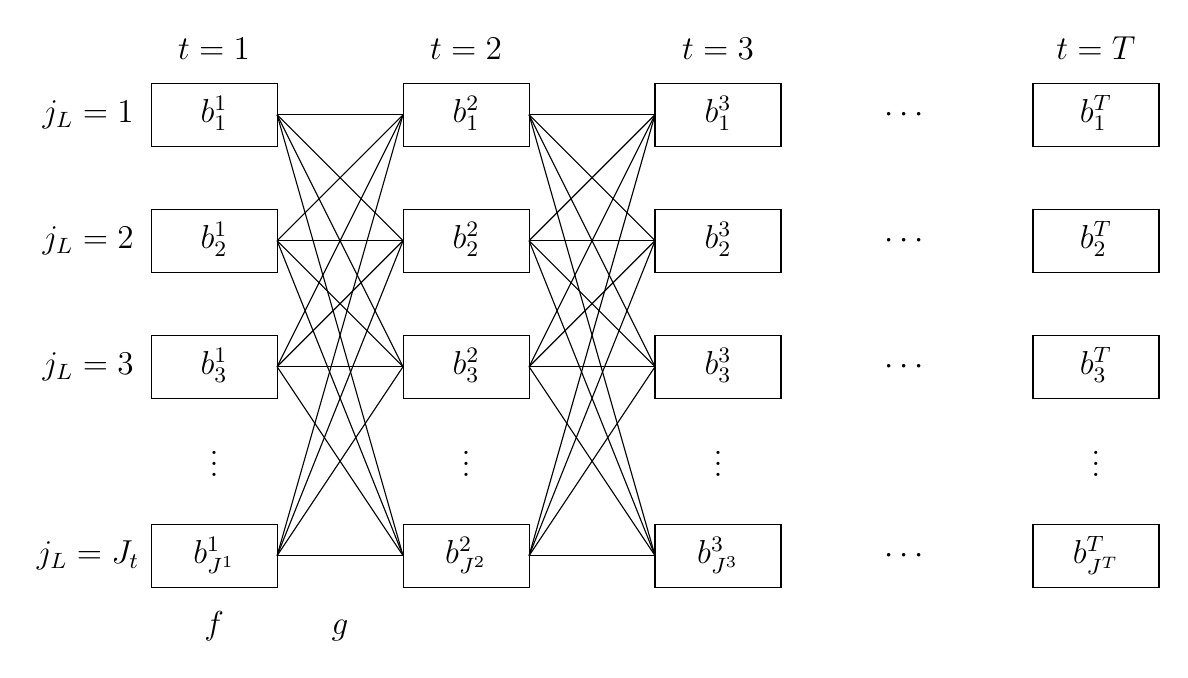
\begin{tikzpicture}[y=-1cm]

% objects at depth 50:
\draw[black] (3.8,4.2) -- (5.4,4.2);
\draw[black] (3.8,2.6) -- (5.4,2.6);
\draw[black] (3.8,5.8) -- (5.4,5.8);
\draw[black] (3.8,8.2) -- (5.4,8.2);
\draw[black] (3.8,2.6) -- (5.4,4.2);
\draw[black] (3.8,2.6) -- (5.4,5.8);
\draw[black] (3.8,2.6) -- (5.4,8.2);
\draw[black] (3.8,4.2) -- (5.4,2.6);
\draw[black] (3.8,4.2) -- (5.4,5.8);
\draw[black] (3.8,4.2) -- (5.4,8.2);
\draw[black] (3.8,5.8) -- (5.4,2.6);
\draw[black] (3.8,5.8) -- (5.4,4.2);
\draw[black] (3.8,5.8) -- (5.4,8.2);
\draw[black] (3.8,8.2) -- (5.4,2.6);
\draw[black] (3.8,8.2) -- (5.4,4.2);
\draw[black] (3.8,8.2) -- (5.4,5.8);
\draw[black] (7,4.2) -- (8.6,4.2);
\draw[black] (7,2.6) -- (8.6,2.6);
\draw[black] (7,5.8) -- (8.6,5.8);
\draw[black] (7,8.2) -- (8.6,8.2);
\draw[black] (7,2.6) -- (8.6,4.2);
\draw[black] (7,2.6) -- (8.6,5.8);
\draw[black] (7,2.6) -- (8.6,8.2);
\draw[black] (7,4.2) -- (8.6,2.6);
\draw[black] (7,4.2) -- (8.6,5.8);
\draw[black] (7,4.2) -- (8.6,8.2);
\draw[black] (7,5.8) -- (8.6,2.6);
\draw[black] (7,5.8) -- (8.6,4.2);
\draw[black] (7,5.8) -- (8.6,8.2);
\draw[black] (7,8.2) -- (8.6,2.6);
\draw[black] (7,8.2) -- (8.6,4.2);
\draw[black] (7,8.2) -- (8.6,5.8);
\draw[black] (2.2,2.2) rectangle (3.8,3);
\draw[black] (2.2,3.8) rectangle (3.8,4.6);
\draw[black] (2.2,5.4) rectangle (3.8,6.2);
\draw[black] (2.2,7.8) rectangle (3.8,8.6);
\path (3,7.2) node[text=black,anchor=base] {\large{}$\vdots$};
\draw[black] (8.6,2.2) rectangle (10.2,3);
\draw[black] (8.6,3.8) rectangle (10.2,4.6);
\draw[black] (8.6,5.4) rectangle (10.2,6.2);
\draw[black] (8.6,7.8) rectangle (10.2,8.6);
\path (9.4,7.2) node[text=black,anchor=base] {\large{}$\vdots$};
\draw[black] (13.4,2.2) rectangle (15,3);
\draw[black] (13.4,3.8) rectangle (15,4.6);
\draw[black] (13.4,5.4) rectangle (15,6.2);
\draw[black] (13.4,7.8) rectangle (15,8.6);
\path (14.2,7.2) node[text=black,anchor=base] {\large{}$\vdots$};
\draw[black] (5.4,2.2) rectangle (7,3);
\draw[black] (5.4,3.8) rectangle (7,4.6);
\draw[black] (5.4,5.4) rectangle (7,6.2);
\draw[black] (5.4,7.8) rectangle (7,8.6);
\path (6.2,7.2) node[text=black,anchor=base] {\large{}$\vdots$};
\path (3,9.2) node[text=black,anchor=base] {\large{}$f$};
\path (4.6,9.2) node[text=black,anchor=base] {\large{}$g$};
\path (3,1.9) node[text=black,anchor=base] {\large{}$t=1$};
\path (6.2,1.9) node[text=black,anchor=base] {\large{}$t=2$};
\path (9.4,1.9) node[text=black,anchor=base] {\large{}$t=3$};
\path (14.2,1.9) node[text=black,anchor=base] {\large{}$t=T$};
\path (1.4,2.7) node[text=black,anchor=base] {\large{}$j_L=1$};
\path (1.4,5.9) node[text=black,anchor=base] {\large{}$j_L=3$};
\path (1.4,4.3) node[text=black,anchor=base] {\large{}$j_L=2$};
\path (1.4,8.3) node[text=black,anchor=base] {\large{}$j_L=J_t$};
\path (3,2.7) node[text=black,anchor=base] {\large{}$b^1_1$};
\path (3,4.3) node[text=black,anchor=base] {\large{}$b^1_2$};
\path (3,5.9) node[text=black,anchor=base] {\large{}$b^1_3$};
\path (6.2,2.7) node[text=black,anchor=base] {\large{}$b^2_1$};
\path (6.2,4.3) node[text=black,anchor=base] {\large{}$b^2_2$};
\path (6.2,5.9) node[text=black,anchor=base] {\large{}$b^2_3$};
\path (9.4,2.7) node[text=black,anchor=base] {\large{}$b^3_1$};
\path (9.4,4.3) node[text=black,anchor=base] {\large{}$b^3_2$};
\path (9.4,5.9) node[text=black,anchor=base] {\large{}$b^3_3$};
\path (14.2,2.7) node[text=black,anchor=base] {\large{}$b^T_1$};
\path (14.2,4.3) node[text=black,anchor=base] {\large{}$b^T_2$};
\path (14.2,5.9) node[text=black,anchor=base] {\large{}$b^T_3$};
\path (3,8.3) node[text=black,anchor=base] {\large{}$b^1_{J^1}$};
\path (6.2,8.3) node[text=black,anchor=base] {\large{}$b^2_{J^2}$};
\path (9.4,8.3) node[text=black,anchor=base] {\large{}$b^3_{J^3}$};
\path (14.2,8.3) node[text=black,anchor=base] {\large{}$b^T_{J^T}$};
\path (11.8,2.7) node[text=black,anchor=base] {\large{}$\cdots$};
\path (11.8,4.3) node[text=black,anchor=base] {\large{}$\cdots$};
\path (11.8,5.9) node[text=black,anchor=base] {\large{}$\cdots$};
\path (11.8,8.3) node[text=black,anchor=base] {\large{}$\cdots$};

\end{tikzpicture}%
}\\[-0.5ex]
      &\raisebox{5pt}{{\huge $\times$}}&\\[-0.5ex]
      \scalebox{0.17}{\input{figures/sentence-tracker-1}}&
      \raisebox{15pt}{{\Large $\times\cdots\times$}}&
      \scalebox{0.17}{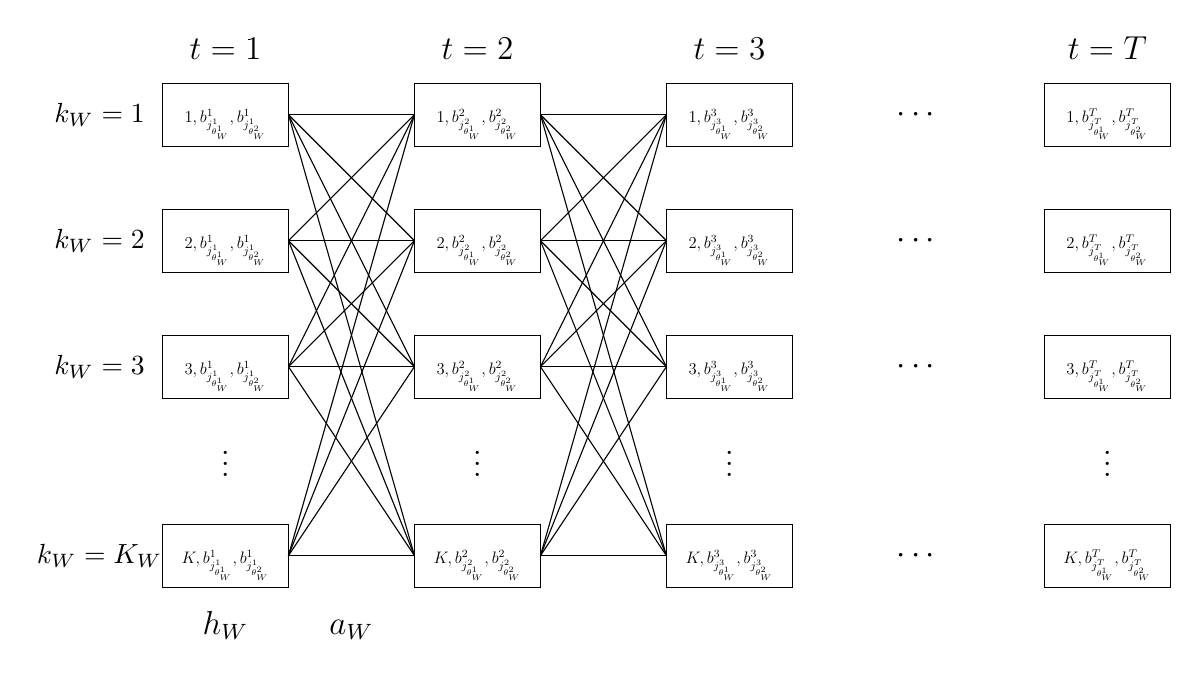
\begin{tikzpicture}[y=-1cm]

% objects at depth 50:
\draw[black] (3.8,4.2) -- (5.4,4.2);
\draw[black] (3.8,2.6) -- (5.4,2.6);
\draw[black] (3.8,5.8) -- (5.4,5.8);
\draw[black] (3.8,8.2) -- (5.4,8.2);
\draw[black] (3.8,2.6) -- (5.4,4.2);
\draw[black] (3.8,2.6) -- (5.4,5.8);
\draw[black] (3.8,2.6) -- (5.4,8.2);
\draw[black] (3.8,4.2) -- (5.4,2.6);
\draw[black] (3.8,4.2) -- (5.4,5.8);
\draw[black] (3.8,4.2) -- (5.4,8.2);
\draw[black] (3.8,5.8) -- (5.4,2.6);
\draw[black] (3.8,5.8) -- (5.4,4.2);
\draw[black] (3.8,5.8) -- (5.4,8.2);
\draw[black] (3.8,8.2) -- (5.4,2.6);
\draw[black] (3.8,8.2) -- (5.4,4.2);
\draw[black] (3.8,8.2) -- (5.4,5.8);
\draw[black] (7,4.2) -- (8.6,4.2);
\draw[black] (7,2.6) -- (8.6,2.6);
\draw[black] (7,5.8) -- (8.6,5.8);
\draw[black] (7,8.2) -- (8.6,8.2);
\draw[black] (7,2.6) -- (8.6,4.2);
\draw[black] (7,2.6) -- (8.6,5.8);
\draw[black] (7,2.6) -- (8.6,8.2);
\draw[black] (7,4.2) -- (8.6,2.6);
\draw[black] (7,4.2) -- (8.6,5.8);
\draw[black] (7,4.2) -- (8.6,8.2);
\draw[black] (7,5.8) -- (8.6,2.6);
\draw[black] (7,5.8) -- (8.6,4.2);
\draw[black] (7,5.8) -- (8.6,8.2);
\draw[black] (7,8.2) -- (8.6,2.6);
\draw[black] (7,8.2) -- (8.6,4.2);
\draw[black] (7,8.2) -- (8.6,5.8);
\draw[black] (5.4,2.2) rectangle (7,3);
\draw[black] (5.4,3.8) rectangle (7,4.6);
\draw[black] (5.4,5.4) rectangle (7,6.2);
\draw[black] (5.4,7.8) rectangle (7,8.6);
\path (6.2,7.2) node[text=black,anchor=base] {\large{}$\vdots$};
\draw[black] (8.6,2.2) rectangle (10.2,3);
\draw[black] (8.6,3.8) rectangle (10.2,4.6);
\draw[black] (8.6,5.4) rectangle (10.2,6.2);
\draw[black] (8.6,7.8) rectangle (10.2,8.6);
\path (9.4,7.2) node[text=black,anchor=base] {\large{}$\vdots$};
\draw[black] (2.2,2.2) rectangle (3.8,3);
\draw[black] (2.2,3.8) rectangle (3.8,4.6);
\draw[black] (2.2,5.4) rectangle (3.8,6.2);
\draw[black] (2.2,7.8) rectangle (3.8,8.6);
\path (3,7.2) node[text=black,anchor=base] {\large{}$\vdots$};
\draw[black] (13.4,2.2) rectangle (15,3);
\draw[black] (13.4,3.8) rectangle (15,4.6);
\draw[black] (13.4,5.4) rectangle (15,6.2);
\draw[black] (13.4,7.8) rectangle (15,8.6);
\path (14.2,7.2) node[text=black,anchor=base] {\large{}$\vdots$};
\path (3,1.9) node[text=black,anchor=base] {\large{}$t=1$};
\path (6.2,1.9) node[text=black,anchor=base] {\large{}$t=2$};
\path (9.4,1.9) node[text=black,anchor=base] {\large{}$t=3$};
\path (14.2,1.9) node[text=black,anchor=base] {\large{}$t=T$};
\path (1.4,2.7) node[text=black,anchor=base] {$k_W=1$};
\path (1.4,4.3) node[text=black,anchor=base] {$k_W=2$};
\path (1.4,8.3) node[text=black,anchor=base] {$k_W=K_W$};
\path (1.4,5.9) node[text=black,anchor=base] {$k_W=3$};
\path (3,9.2) node[text=black,anchor=base] {\large{}$h_W$};
\path (4.6,9.2) node[text=black,anchor=base] {\large{}$a_W$};
\path (11.8,2.7) node[text=black,anchor=base] {\large{}$\cdots$};
\path (11.8,4.3) node[text=black,anchor=base] {\large{}$\cdots$};
\path (11.8,5.9) node[text=black,anchor=base] {\large{}$\cdots$};
\path (11.8,8.3) node[text=black,anchor=base] {\large{}$\cdots$};
\path (3,2.7) node[text=black,anchor=base] {\large{}\scalebox{0.5}{$1,b^1_{j^1_{\theta^1_W}},b^1_{j^1_{\theta^2_W}}$}};
\path (3,4.3) node[text=black,anchor=base] {\large{}\scalebox{0.5}{$2,b^1_{j^1_{\theta^1_W}},b^1_{j^1_{\theta^2_W}}$}};
\path (3,5.9) node[text=black,anchor=base] {\large{}\scalebox{0.5}{$3,b^1_{j^1_{\theta^1_W}},b^1_{j^1_{\theta^2_W}}$}};
\path (3,8.3) node[text=black,anchor=base] {\large{}\scalebox{0.5}{$K,b^1_{j^1_{\theta^1_W}},b^1_{j^1_{\theta^2_W}}$}};
\path (6.2,2.7) node[text=black,anchor=base] {\large{}\scalebox{0.5}{$1,b^2_{j^2_{\theta^1_W}},b^2_{j^2_{\theta^2_W}}$}};
\path (6.2,4.3) node[text=black,anchor=base] {\large{}\scalebox{0.5}{$2,b^2_{j^2_{\theta^1_W}},b^2_{j^2_{\theta^2_W}}$}};
\path (6.2,5.9) node[text=black,anchor=base] {\large{}\scalebox{0.5}{$3,b^2_{j^2_{\theta^1_W}},b^2_{j^2_{\theta^2_W}}$}};
\path (6.2,8.3) node[text=black,anchor=base] {\large{}\scalebox{0.5}{$K,b^2_{j^2_{\theta^1_W}},b^2_{j^2_{\theta^2_W}}$}};
\path (9.4,2.7) node[text=black,anchor=base] {\large{}\scalebox{0.5}{$1,b^3_{j^3_{\theta^1_W}},b^3_{j^3_{\theta^2_W}}$}};
\path (9.4,4.3) node[text=black,anchor=base] {\large{}\scalebox{0.5}{$2,b^3_{j^3_{\theta^1_W}},b^3_{j^3_{\theta^2_W}}$}};
\path (9.4,5.9) node[text=black,anchor=base] {\large{}\scalebox{0.5}{$3,b^3_{j^3_{\theta^1_W}},b^3_{j^3_{\theta^2_W}}$}};
\path (9.4,8.3) node[text=black,anchor=base] {\large{}\scalebox{0.5}{$K,b^3_{j^3_{\theta^1_W}},b^3_{j^3_{\theta^2_W}}$}};
\path (14.2,2.7) node[text=black,anchor=base] {\large{}\scalebox{0.5}{$1,b^T_{j^T_{\theta^1_W}},b^T_{j^T_{\theta^2_W}}$}};
\path (14.2,4.3) node[text=black,anchor=base] {\large{}\scalebox{0.5}{$2,b^T_{j^T_{\theta^1_W}},b^T_{j^T_{\theta^2_W}}$}};
\path (14.2,5.9) node[text=black,anchor=base] {\large{}\scalebox{0.5}{$3,b^T_{j^T_{\theta^1_W}},b^T_{j^T_{\theta^2_W}}$}};
\path (14.2,8.3) node[text=black,anchor=base] {\large{}\scalebox{0.5}{$K,b^T_{j^T_{\theta^1_W}},b^T_{j^T_{\theta^2_W}}$}};

\end{tikzpicture}%
}\\[-0.5ex]
      word $1$&&word $W$
    \end{tabular}
  \end{center}
  \vspace*{-3ex}
  \caption{The cross-product lattice used by the sentence tracker, consisting
    of~$L$ tracking lattices and~$W$ event-model lattices.}
  \label{fig:sentence-tracker}
  \vspace*{-2ex}
\end{wrapfigure}
%
One would expect that encoding the semantics of a complex sentence such as
\emph{The person to the right of the chair quickly carried the red object
  towards the trash can}, which involves nouns, adjectives, verbs, adverbs, and
spatial-relation and motion prepositions, would provide substantially more
mutual constraint on the \emph{collection} of tracks for the participants than a
single intransitive verb would constrain a single track.
%
We thus extend the approach described above by incorporating a complex
multi-argument predicate that represents the semantics of an entire sentence
instead of one that only represents the semantics of a single intransitive verb.
%
This involves formulating the semantics of other parts of speech, in addition
to intransitive verbs, also as HMMs.
%
We then construct a large cross-product lattice, illustrated in
Fig.~\ref{fig:sentence-tracker}, to support~$L$ tracks and~$W$ words.
%
Each node in this cross-product lattice represents $L$~detections and the
states for~$W$ words.
%
To support~$L$ tracks, we subindex each detection index~$j$ as $j_l$ for
track~$l$.
%
Similarly, to support~$W$ words, we subindex each state index~$k$ as~$k_w$ for
word~$w$ and the HMM parameters~$h$ and~$a$ for word~$w$ as~$h_w$ and~$a_w$.
%
The argument-to-track mappings~$\theta^1_w$ and~$\theta^2_w$ specify the tracks
that fill arguments~1 and~2 (where necessary) of word~$w$ respectively.
%
We then seek a path through this cross-product lattice that optimizes
%
\vspace*{-2ex}
\begin{equation*}
  \max_{\substack{j^1_1,\ldots,j^T_1\\j^1_L,\ldots,j^T_L\\
      k^1_1,\ldots,k^T_1\\k^1_W,\ldots,k^T_W}}
  \sum_{l=1}^L
  \sum_{t=1}^Tf(b^t_{j^t_l})+
  \sum_{t=2}^Tg(b^{t-1}_{j^{t-1}_l},b^t_{j^t_l})+
  \sum_{w=1}^W
  \sum_{t=1}^Th_w(k^t_w,b^t_{j^t_{\theta^1_w}},b^t_{j^t_{\theta^2_w}})+
  \sum_{t=2}^Ta_w(k^{t-1}_w,k^t_w)
\end{equation*}
%
This can also be computed in polynomial time using the Viterbi algorithm.
%
This describes a method by which the function
$\mathcal{S}(D,\Phi)\mapsto(\tau,Z)$, discussed earlier, can be computed, where
$D$~is the collection of detections~$b^t_j$ and~$Z$ is the collection of
tracks~$j^t_l$.

\vspace*{-2ex}
\section{Natural-Language Semantics}
\label{sec:semantics}
\vspace*{-2ex}

The sentence tracker uniformly represents the semantics of words in all parts
of speech, namely nouns, adjectives, verbs, adverbs, and prepositions (both
those that describe spatial relations and those that describe motion), as HMMs.
%
Finite state recognizers (FSMs) are a special case of HMMs where the transition
matrices~$a$ and the output models~$h$ are 0/1.
%
Here, we formulate the semantics of a small fragment of English consisting
of~17 lexical items (5~nouns, 2~adjectives, 4~verbs, 2~adverbs,
2~spatial-relation prepositions, and 2~motion prepositions), by hand, as FSMs.
%
We do so to focus on what once can do with this approach, namely take sentences
as input and focus the attention of a tracker, take video as input and produce
sentential descriptions as output, and perform content-based video retrieval
given a sentential input query, as discussed in Section~\ref{sec:experiments}.
%
It is particularly enlightening that the FSMs we use are perspicuous and
clearly encode pretheoretic human intuitions about the semantics of these words.
%
But nothing turns on the use of hand-coded FSMs.
%
Our framework, as described above, supports HMMs.
%
A companion submission describes a method by which one can automatically learn
such HMMs for the lexicon, grammar, and corpus discussed in this paper.

\begin{table}[t]
  \centering\ra{1.1}
  \begin{tabular}{@{}cc@{}}
    \begin{tabular}{@{}c@{}}
      \scalebox{0.65}{\begin{tabular}{@{}r@{$\;\rightarrow\;$}l@{}}
        S & NP VP\\
        NP & D [A] N [PP]\\
        D & \emph{an} \textbar\ \emph{the}\\
        A & \emph{blue} \textbar\ \emph{red}\\
        N & \emph{person} \textbar\ \emph{backpack} \textbar\ \emph{trash can} \textbar\ \emph{chair} \textbar\ \emph{object}\\
        PP & P NP\\
        P & \emph{to the left of} \textbar\ \emph{to the right of}\\
        VP & V NP [ADV] [PPM]\\
        V & \emph{picked up} \textbar\ \emph{put down} \textbar\ \emph{carried} \textbar\ \emph{approached}\\
        ADV & \emph{quickly} \textbar\ \emph{slowly}\\
        PPM & PM NP\\
        PM & \emph{towards} \textbar\ \emph{away from}
      \end{tabular}}\\
      (a)\\
      \scalebox{0.65}{\begin{tabular}{@{}r@{$\;=\;$}l@{}}
          \emph{to the left of} & (agent patient) (referent)\\
          \emph{to the right of} & (agent patient) (referent)\\
          \emph{picked up} & (agent) (patient)\\
          \emph{put down} & (agent) (patient)\\
          \emph{carried} & (agent) (patient)\\
          \emph{approached} & (agent) (goal)\\
          \emph{towards} & (agent patient) (goal)\\
          \emph{away from} & (agent patient) (source)\\
          other & (agent patient referent goal source)\\
      \end{tabular}}\\
      (b)
    \end{tabular}&
  \begin{tabular}{@{}c@{}}
    \scalebox{0.7}{\begin{tabular}{@{}r@{}l@{.\hspace{1ex}}l@{}}
        1&a&\emph{The backpack approached the trash can.}\\
        &b&\emph{The chair approached the trash can.}\\
        2&a&\emph{The red object approached the chair.}\\
        &b&\emph{The blue object approached the chair.}\\
        3&a&\emph{The person to the left of the trash can put down an object.}\\
        &b&\emph{The person to the right of the trash can put down an object.}\\
        4&a&\emph{The person put down the trash can.}\\
        &b&\emph{The person put down the backpack.}\\
        5&a&\emph{The person carried the red object.}\\
        &b&\emph{The person carried the blue object.}\\
        6&a&\emph{The person picked up an object to the left of the trash can.}\\
        &b&\emph{The person picked up an object to the right of the trash can.}\\
        7&a&\emph{The person picked up an object.}\\
        &b&\emph{The person put down an object.}\\
        8&a&\emph{The person picked up an object quickly.}\\
        &b&\emph{The person picked up an object slowly.}\\
        9&a&\emph{The person carried an object towards the trash can.}\\
        &b&\emph{The person carried an object away from the trash can.}\\
        1&0&\emph{The backpack approached the chair.}\\
        1&1&\emph{The red object approached the trash can.}\\
        1&2&\emph{The person put down the chair.}
    \end{tabular}}\\
    (c)
    \end{tabular}
  \end{tabular}
  \vspace*{-2ex}
  \caption{(a) The grammar for our lexicon of 19 lexical entries (2
    determiners, 2 adjectives, 5 nouns, 2 spatial relations, 4 verbs, 2
    adverbs, and 2 motion prepositions).
    %
    Note that the grammar allows for infinite recursion in the noun phrase.
    %
    (b) The theta grid, specifying the number of arguments and
    roles such arguments refer to, for our lexicon.
    %
    (c) A selection of sentences drawn from the grammar based on which we
    collected (multiple instances of) videos for our experimental corpus..  }
  \label{tab:language}
  \vspace*{-3ex}
\end{table}

Nouns (\eg\ \emph{person}) may be represented by constructing static FSMs over
discrete features, such as detector class.
%
Adjectives (\eg\ \emph{red}, \emph{tall}, and \emph{big}) may be represented as
static FSMs that describe select properties of the detections for a single
participant, such as color, shape, or size, independent of other features of
the overall event.
%
Intransitive verbs (\eg\ \emph{bounce}) may be represented as FSMs that
describe the changing motion characteristics of a single participant, such as
\emph{moving downward} followed by \emph{moving upward}.
%
Transitive verbs (\eg\ \emph{approach}) may be represented as FSMs that
describe the changing relative motion characteristics of two participants, such
as \emph{moving closer}.
%
Adverbs (\eg\ \emph{slowly} and \emph{quickly}) may be represented by FSMs that
describe the velocity of a single participant, independent of the direction of
motion.
%
Spatial-relation prepositions (\eg\ \emph{to the left of}) may be represented
as static FSMs that describe the relative position of two participants.
%
Motion prepositions (\eg\ \emph{towards} and \emph{away from}) may be
represented as FSMs that describe the changing relative position of two
participants.
%
As is often the case, even simple static properties, such as detector class,
object color, shape, and size, spatial relations, and direction of motion,
might hold only for a portion of an event.
%
We handle such temporal uncertainty by incorporating garbage states into the
FSMs that always accept and do not affect the scores computed.
%
This also allows for alignment between multiple words in a temporal interval
during a longer aggregate event.
%
Table~\ref{tab:predicates} provides, in the form of predicates and regular
expressions describing the FSMs, the complete specification of lexical
semantics for the grammar and lexicon presented in Table~\ref{tab:language}(a).

\begin{table}
  \centering\ra{1.1}
  \scalebox{0.5}{\begin{tabular}{@{}c@{}}
      \begin{tabular}{@{\hspace{0ex}}c@{\hspace{0ex}}c@{\hspace{0ex}}c@{\hspace{0ex}}}
        \midrule Constants & Simple Predicates & Complex Predicates\\ \midrule \addlinespace[1ex]
        \begin{math}
          \begin{array}[t]{r@{\;\define\;}l}
            \textsc{xBoundary} & 300\textsc{px}\\
            \textsc{nextTo} & 50\textsc{px}\\
            \Delta\textsc{static} & 6\textsc{px}\\
            \Delta\textsc{jump} & 30\textsc{px}\\
            \Delta\textsc{quick} & 80\textsc{px}\\
            \Delta\textsc{slow} & 30\textsc{px}\\
            \Delta\textsc{closing} & 10\textsc{px}\\
            \Delta\textsc{direction} & 30\degr\\
            \Delta\textsc{hue} & 30\degr
          \end{array}
        \end{math} &
        \begin{math}
          \begin{array}[t]{r@{\;\define\;}l}
            \textsc{xDistance}(P,Q) &
            \lvert x(p^t)-x(q^t) \rvert\\
            \textsc{noJitter}(P,v) &
            \lvert c(p^t)\cdot v-c(p^{t-1})\cdot v\rvert\le\Delta\textsc{jump}\\
            \textsc{alike}(P,Q) &
            \textit{model}(p^t)=\textit{model}(q^t)\\
            \textsc{far}(P,Q) &
            \textsc{xDistance}(P,Q)\ge\textsc{xBoundary}\\
            \textsc{close}(P,Q) &
            \textsc{xDistance}(P,Q)<\textsc{xBoundary}\\
            \textsc{left}(P,Q) &
            0<x(q^t)-x(p^t)\le\textsc{nextTo}\\
            \textsc{right}(P,Q) &
            0<x(p^t)-x(q^t)\le\textsc{nextTo}\\
            \textsc{hasColour}(P,\textrm{hue}) &
            \textsc{angleSep}(\textit{hue}(p^t),\textrm{hue})\le
            \Delta\textsc{hue}\\
            \textsc{quick}(P) &
            \lvert p^t-p^{t-1}\rvert\ge\Delta\textsc{quick}\\
            \textsc{slow}(P) &
            \lvert p^t-p^{t-1}\rvert\le\Delta\textsc{slow}\\
            \textsc{stationary}(P) &
            \lVert\textsc{avgFlow}(p^t)\rVert\le\Delta\textsc{static}
          \end{array}
        \end{math}&
        \begin{math}
          \begin{array}[t]{r@{\;\define\;}l}
            \textsc{stationaryClose}(P,Q) &
            \textsc{stationary}(P)\conjunct
            \textsc{stationary}(Q)\conjunct
            \neg\textsc{alike}(P,Q)\conjunct
            \textsc{close}(P,Q)\\
            \textsc{stationaryFar}(P,Q) &
            \textsc{stationary}(P)\conjunct
            \textsc{stationary}(Q)\conjunct
            \neg\textsc{alike}(P,Q)\conjunct
            \textsc{far}(P,Q)\\
            \textsc{closer}(P,Q) &
            \textsc{xDistance}(P,Q)>\textsc{xDistance}(\textsc{fwdProj}(P),Q)+
            \Delta\textsc{closing}\\
            \textsc{farther}(P,Q) &
            \textsc{xDistance}(P,Q)<\textsc{xDistance}(\textsc{fwdProj}(P),Q)+
            \Delta\textsc{closing}\\
            \textsc{moveCloser}(P,Q) &
            \textsc{noJitter}(P,(0,1))\conjunct
            \textsc{noJitter}(Q,(0,1))\conjunct
            \textsc{closer}(P,Q)\\
            \textsc{moveFarther}(P,Q) &
            \textsc{noJitter}(P,(0,1))\conjunct
            \textsc{noJitter}(Q,(0,1))\conjunct
            \textsc{farther}(P,Q)\\
            \textsc{alongDir}(P,v) &
            \textsc{angleSep}(\angle\textsc{avgFlow}(p^t),\angle v)<
            \Delta\textsc{direction}\conjunct
            \neg\textsc{stationary}(P)\\
            \textsc{movingDir}(P,v) &
            \textsc{alongDir}(P,v)\conjunct\textsc{noJitter}(P,normal(v))\\
            \textsc{approaching}(P,Q) &
            \neg\textsc{alike}(P,Q)\conjunct
            \textsc{stationary}(Q)\conjunct
            \textsc{moveCloser}(P,Q)\\
            \textsc{departing}(P,Q) &
            \neg\textsc{alike}(P,Q)\conjunct
            \textsc{stationary}(Q)\conjunct
            \textsc{moveFarther}(P,Q)\\
            \textsc{pickingUp}(P,Q) &
            \neg\textsc{alike}(P,Q)\conjunct
            \textsc{stationary}(P)\conjunct
            \textsc{movingDir}(P,(0,1))\\
            \textsc{puttingDown}(P,Q) &
            \neg\textsc{alike}(P,Q)\conjunct
            \textsc{stationary}(P)\conjunct
            \textsc{movingDir}(P,(0,-1))\\
            \textsc{carry}(P,Q,v) &
            \textsc{movingDir}(P,v)\conjunct\textsc{movingDir}(Q,v)\\
            \textsc{carrying}(P,Q) &
            \textsc{carry}(P,Q,(0,1))\disjunct\textsc{carry}(P,Q,(0,-1))\\
          \end{array}
        \end{math}
      \end{tabular}\\
      \addlinespace[1ex] \midrule Regular Expressions\\ \midrule \addlinespace[1ex]
      \begin{tabular}{@{}c@{\hspace{8ex}}c@{}}
        \begin{math}
          \begin{array}[t]{r@{\;\define\;}l}
            \textsc{person}(P) &
            (\textit{model}(p^t)=\textbf{person})\plus\\
            \textsc{backpack}(P) &
            (\textit{model}(p^t)=\textbf{backpack})\plus\\
            \textsc{trashCan}(P) &
            (\textit{model}(p^t)=\textbf{trashCan})\plus\\
            \textsc{chair}(P) &
            (\textit{model}(p^t)=\textbf{chair})\plus\\
            \textsc{blue}(P) &
            \textsc{hasColour}(P,225^\circ)\plus\\
            \textsc{red}(P) &
            \textsc{hasColour}(P,0^\circ)\plus\\
            \textsc{quickly}(P) &
            \textsc{true}\plus\;\textsc{quick}(P)\dagr\;\textsc{true}\plus\\
            \textsc{slowly}(P) &
            \textsc{true}\plus\;\textsc{slow}(P)\dagr\;\textsc{true}\plus\\
            \textsc{toTheLeftOf}(P,Q) & \textsc{left}(P,Q)\plus\\
            \textsc{toTheRightOf}(P,Q) & \textsc{right}(P,Q)\plus
          \end{array}
        \end{math}&
        \begin{math}
          \begin{array}[t]{r@{\;\define\;}l}
            \textsc{pickedUp}(P,Q) &
            \textsc{stationaryClose}(P,Q)\plus\;
            \textsc{pickingUp}(P,Q)\dagr\;
            \textsc{stationaryClose}(P,Q)\plus\\
            \textsc{putDown}(P,Q) &
            \textsc{stationaryClose}(P,Q)\plus\;
            \textsc{puttingDown}(P,Q)\dagr\;
            \textsc{stationaryClose}(P,Q)\plus\\
            \textsc{carried}(P,Q) &
            \textsc{stationaryClose}(P,Q)\plus\;
            \textsc{carrying}(P,Q)\dagr\;
            \textsc{stationaryClose}(P,Q)\plus\\
            \textsc{approached}(P,Q) &
            \textsc{stationaryFar}(P,Q)\plus\;
            \textsc{approaching}(P,Q)\dagr\;
            \textsc{stationaryClose}(P,Q)\plus\\
            \textsc{towards}(P,Q) &
            \textsc{stationaryFar}(P,Q)\plus\;
            \textsc{approaching}(P,Q)\dagr\;
            \textsc{stationaryClose}(P,Q)\plus\\
            \textsc{awayFrom}(P,Q) &
            \textsc{stationaryClose}(P,Q)\plus\;
            \textsc{departing}(P,Q)\dagr\;
            \textsc{stationaryFar}(P,Q)\plus\\
            \textsc{object}(P) &
            (\textit{model}(p^t)=\textbf{backpack}
            \disjunct\textit{model}(p^t)=\textbf{trashcan}
            \disjunct\textit{model}(p^t)=\textbf{chair})\plus
          \end{array}
        \end{math}
      \end{tabular}
    \end{tabular}}
  \caption{The finite-state recognizers corresponding to the lexicon in
    Table~\protect\ref{tab:language}(a).
    %
    Here, we denote a track (sequence of detections) as
    $P = \langle p^1,\ldots,p^t\rangle$,
    $t$~being the most recent detection.
    %
    Features for a detection are computed using the functions~$c$, $x$, and
    $model$ that compute its center, x-coordinate of the center, and the
    associated object-model name respectively.
    %
    $v$~denotes a unit vector used to indicate direction.
    %
    $\textsc{avgFlow}$ and $\textsc{fwdProj}$ are computed based on the
    aggregate optical flow within a detection's bounding area in an image.
    %
    The former returns a vector (magnitude and orientation) and the latter
    displaces a given detection by this vector.
    %
    Finally, we define a new regular expression quantifier $\dagger$ as
    $\textsc{R}\dagr=(\textsc{R}\;\textsc{true}^?\;\textsc{R})\plus$ to
    support handling noisy data.
  }
  \label{tab:predicates}
  \vspace*{-3ex}
\end{table}

A sentence may describe an activity involving multiple tracks, where different
(collections of) tracks fill the arguments of different words.
%
This gives rise to the requirement of compositional semantics: dealing with the
mappings from arguments to tracks.
%
Given a sentence, say \emph{The person to the right of the chair picked up the
  backpack}, argument-to-track assignment is a function
$\mathcal{T}(\Lambda,\Gamma,\Psi)\mapsto(\Phi)$, that takes, as input, a
sentence~$\Lambda$ and a grammar~$\Gamma$, along with a specification of the
argument arity and role types~$\Psi$ for the words in the lexicon and produces
a formula~$\Phi$ that specifies which tracks fill which arguments of which
predicate instances for the words in the sentence.
%
Such a function, applied to our example sentence with the grammar~$\Gamma$ as
specified in Table~\ref{tab:language}(a) and \defoccur{theta grid}~$\Psi$, as
specified in Table~\ref{tab:language}(b), would produce the following formula.
%
\begin{equation*}
  \textsc{person}(P) \wedge
  \textsc{toTheRightOf}(P,Q)\wedge
  \textsc{chair}(Q) \wedge
  \textsc{pickedUp}(P,R)\wedge
  \textsc{backpack}(R)
\end{equation*}
%
% needs work: citation for government and lexical binding?
%
\begin{wrapfigure}{r}{0.32\textwidth}
  \vspace*{-2ex}
  \scalebox{0.55}{%
    \Tree [.S [.NP [.N {\it person} ]
    [.PP [.P {\it to the right of} ]
    [.N {\it chair} ]]]
    [.VP [.V {\it picked up} ]
    [.NP [.N {\it backpack} ]]]]
  }
  \vspace*{-2ex}
\end{wrapfigure}
%
To do so, we first construct a parse tree of the sentence~$\Lambda$ given the
grammar~$\Gamma$, using a recursive-descent parser, producing
the parse tree shown.
%
Such a parse tree encodes in its structure, the dependency relationships
between different parts of speech as specified by the grammar.
%
For each word, we then determine from the parse tree, which words in the
sentence are determined to be its \textsl{dependents} in the sense of
\textsl{government}, and how many such \textsl{dependents} exist, from the
theta grid specified in Table~\ref{tab:language}(b).
%
For example, the dependents of \emph{to the right of} are determined to be
\emph{person} and \emph{chair}, filling its first and second arguments
respectively.
%
Furthermore, we determine a consistent assignment of roles, one of agent,
patient, source, goal, and referent, for each participant track that fills the
word arguments, from the allowed roles specified for that word
and argument in the theta grid.
%
Here, $P$, $Q$, and~$R$ are participants that play the agent, referent, and
patient roles respectively.

\vspace*{-2ex}
\section{Experimental Evaluation}
\label{sec:experiments}
\vspace*{-2ex}

The sentence tracker supports three distinct capabilities.
%
It can take sentences as input and focus the attention of a tracker, it can
take video as input and produce sentential descriptions as output, and it can
perform content-based video retrieval given a sentential input query.
%
To evaluate these, we filmed a corpus of~94 short videos, of varying
length, in~3 different outdoor environments.
%
The camera was moved for each video so that the varying background
precluded unanticipated confounds.
%
These videos, filmed with a variety of actors, each depicted one or more of
the~21 sentences from Table~\ref{tab:language}(c).
%
The depiction, from video to video, varied in scene layout and the actor(s)
performing the event.
%
The corpus was carefully constructed in a number of ways.
%
First, many videos depict more than one sentence.
%
In particular, many videos depict simultaneous distinct events.
%
Second, each sentence is depicted by multiple videos.
%
Third the corpus was constructed with minimal pairs: pairs of videos whose
depicted sentences differ in exactly one word.
%
These minimal pairs are indicated as the `a' and `b' variants of sentences 1--9
in Table~\ref{tab:language}(c).
%
That varying word was carefully chosen to span all parts of speech and all
sentential positions: sentence~1 varies subject noun, sentence~2 varies subject
adjective, sentence~3 varies subject preposition, sentence~4 varies object
noun, sentence~5 varies object adjective, sentence~6 varies object preposition,
sentence~7 varies verb, sentence~8 varies adverb, and sentence~9 varies
motion preposition.
%
We filmed our own corpus as we are unaware of any existing corpora that exhibit
the above properties.
%
We annotated each of the~94 clips with a ground truth judgment for each of
the~21 sentences, indicating whether the given clip depicted the given
sentence.
%
This set of~1974 judgments was used for the following analyses.

\vspace*{-3ex}
\subsection{Focus of Attention}
\label{subsec:foa}
\vspace*{-2ex}

Tracking is traditionally performed using cues from motion, object detection,
or manual initialization on an object of interest.
%
However, in the case of a cluttered scene involving multiple activities
occurring simultaneously, there can be many moving objects, many instances of
the same object class, and perhaps even multiple simultaneously occurring
instances of the same event class.
%
This presents a significant obstacle to the efficacy of existing methods in
such scenarios.
%
To alleviate this problem, one can decide which objects to track based on which
ones participate in a target event.

The sentence tracker can focus its attention on just those objects that
participate in an event specified by a sentential description.
%
Such a description can differentiate between different simultaneous events
taking place between many moving objects in the scene using descriptions
constructed out of a variety of parts of speech: nouns to specify object class,
adjectives to specify object properties, verbs to specify events, adverbs to
specify motion properties, and prepositions to specify (changing) spatial
relations between objects.
%
Furthermore, such a sentential description can even differentiate which objects
to track based on the role that they play in an event: agent, patient, source,
goal, or referent.
%
Fig.~\ref{fig:inference} demonstrates this ability: different tracks are
produced for the same video that depicts multiple simultaneous events when
focused with different sentences.

% needs work: regenerate all images without captions

\begin{figure}
  \centering
  \begin{tabular}
    {@{}c@{\hspace{5pt}}c@{\hspace{5pt}}c@{\hspace{5pt}}c@{\hspace{5pt}}c@{}}
    \includegraphics[width=0.19\textwidth]{images/inference1a-0004}&
    \includegraphics[width=0.19\textwidth]{images/inference1a-0005}&
    \includegraphics[width=0.19\textwidth]{images/inference1a-0006}&
    \includegraphics[width=0.19\textwidth]{images/inference1a-0008}&
    \includegraphics[width=0.19\textwidth]{images/inference1a-0010}\\
    \multicolumn{5}{@{}l}{\emph{The person picked up an object.}}\\[1ex]
    \includegraphics[width=0.19\textwidth]{images/inference1b-0001}&
    \includegraphics[width=0.19\textwidth]{images/inference1b-0003}&
    \includegraphics[width=0.19\textwidth]{images/inference1b-0004}&
    \includegraphics[width=0.19\textwidth]{images/inference1b-0006}&
    \includegraphics[width=0.19\textwidth]{images/inference1b-0008}\\
    \multicolumn{5}{@{}l}{\emph{The person put down an object.}}\\
  \end{tabular}
  \vspace*{-2ex}
  \caption{Sentence-guided focus of attention: two different sets of tracks for
    the same video produced under guidance of two different sentences.}
  \label{fig:inference}
  \vspace*{-5ex}
\end{figure}

We further evaluated this ability on all~9 minimal pairs collectively applied
to all~24 suitable videos in our corpus.
%
For 21~out of the~24, both sentences in the minimal pair yielded tracks deemed
to be correct depictions.
%
We include example videos for all~9 minimal pairs in the supplementary material.

\vspace*{-2ex}
\subsection{Generation}
\label{subsec:generation}
\vspace*{-2ex}

Much of the prior work on generating sentences to describe images
\citep{Jie2009, Farhadi2010, Li2011a, Yang2011, Gupta2012, Mitchell2012} and
video \citep{Kojima2002, Tena2007, Barbu2012a, Khan2012, Wang2012} uses
special-purpose natural-language-generation methods.
%
We can instead use the ability of the sentence tracker to score a sentence
paired with a video as a general-purpose natural-language generator by
searching for the highest-scoring sentence for a given video.
%
However, this has a problem.
%
Since~$h$ and~$a$ are $\log$ probabilities, $g$~is a negative Euclidean
distance, and we constrain~$f$ to be negative, scores decrease with longer word
strings and greater numbers of tracks that result from longer word strings.
%
So we don't actually search for the highest-scoring sentence, which would bias
the process towards short sentences.
%
Instead we seek complex sentences that are true of the video as they are more
informative.

Nominally, this search process would be intractable since the space of possible
sentences can be huge and even infinite.
%
However, we can use beam search to get an approximate answer.
%
This is possible because the sentence tracker can score any collection of
words, not just complete phrases or sentences.
%
We can select the~$k$ top-scoring single-word strings and then repeatedly
extend the~$k$ top-scoring $n$-word strings, by one word, to select the~$k$
top-scoring $n+1$-word strings, subject to the constraint that these $n+1$-word
strings can be extended to grammatical sentences by insertion of additional
words.
%
Thus we terminate the search process when the \defoccur{contraction threshold},
the ratio between the score of an expanded string and the score of the string
it expanded from, exceeds a specified value and the string being expanded is a
complete sentence.
%
This contraction threshold controls complexity of the generated sentence.

When restricted to FSMs, $h$~and~$a$ will be 0/1 which become $-\infty$/0
in $\log$ space.
%
Thus increase in the number of words can only decrease a score to $-\infty$,
meaning that a string of words is no-longer true of a video.
%
Since we seek true sentences, we terminate the above beam search process before
the score goes to $-\infty$.
%
In this case, there is no approximation: a beam search maintaining all $n$-word
strings with finite score yields the highest-scoring sentence before the
contraction threshold is met.

% needs work: regenerate all images without captions

\begin{figure}
  \centering
  \begin{tabular}
    {@{}c@{\hspace{5pt}}c@{\hspace{5pt}}c@{\hspace{5pt}}c@{\hspace{5pt}}c@{}}
    \includegraphics[width=0.19\textwidth]{images/generation2-0003}&
    \includegraphics[width=0.19\textwidth]{images/generation2-0005}&
    \includegraphics[width=0.19\textwidth]{images/generation2-0006}&
    \includegraphics[width=0.19\textwidth]{images/generation2-0007}&
    \includegraphics[width=0.19\textwidth]{images/generation2-0009}\\
    \multicolumn{5}{@{}l}{\emph{The backpack approached the trash can.}}\\[1ex]
    \includegraphics[width=0.19\textwidth]{images/generation1-0001}&
    \includegraphics[width=0.19\textwidth]{images/generation1-0005}&
    \includegraphics[width=0.19\textwidth]{images/generation1-0006}&
    \includegraphics[width=0.19\textwidth]{images/generation1-0008}&
    \includegraphics[width=0.19\textwidth]{images/generation1-0010}\\
    \multicolumn{5}{@{}l}{\emph{The person to the left of the trash can put down
        the chair.}}\\
  \end{tabular}
  \vspace*{-2ex}
  \caption{Generation of sentential descriptions: constructing the
    highest-scoring sentence for each video that is generated by the grammar in
    Table~\protect\ref{tab:language}(a), by means of a beam search.}
  \label{fig:generation}
  \vspace*{-4ex}
\end{figure}

To evaluate this approach, we searched the space of sentences in the grammar in
Table~\ref{tab:language}(a) to find the best true sentence for each of the~94
videos in our corpus.
%
Note that the grammar generates an infinite number of sentences due to
recursion in NP.\@
%
Even restricting the grammar to eliminate NP recursion yields a space of
816,419,347,200 sentences.
%
Despite not restricting the grammar in this fashion, we are able to effectively
find good descriptions of the videos.
%
We computed the accuracy of the sentence tracker in generating descriptions for
all~94 videos in our corpus for multiple contraction thresholds.
%
Accuracy was computed as the percentage of the~94 videos for which the
sentence tracker produced descriptions that were deemed to be true.
%
Contraction thresholds of 0.95, 0.90, and 0.85 yielded accuracies of
63.82\%, 69.14\%, and 64.89\% respectively.
%
We demonstrate examples of this approach in Fig.~\ref{fig:generation}.
%
The supplementary material contains additional examples.

\vspace*{-2ex}
\subsection{Retrieval}
\label{subsec:retrieval}
\vspace*{-2ex}

The availability of vast video corpora, such as on YouTube, has created a
rapidly growing demand for content-based video search and retrieval.
%
The existing systems, however, only provide a means to search via human-provided
captions.
%
The inefficacy of such an approach is evident.
%
Attempting to search for even simple queries such as \emph{pick up} or
\emph{put down} yields surprisingly poor results, let alone searching for more
complex queries such as \emph{person approached horse}.
%
Furthermore, prior work on content-based video-retrieval systems like
\citet{Sivic2003} search only for objects and like \citet{laptev:08} search
only for events.
%
Even combining such to support conjunctive queries for videos with specified
collections of objects jointly with a specified event, would not effectively
rule out videos where the specified objects did not play a role in the event or
played different roles in the event.
%
For example, it could not rule out a video depicting a person jumping next to a
stationary ball for a query \emph{ball bounce} or distinguish between the
queries \emph{person approached horse} and \emph{horse approached person}.
%
The sentence tracker exhibits the ability to serve as the basis of a much
better video search and retrieval tool, one that performs content-based search
with complex sentential queries to find precise semantically relevant clips,
as demonstrated in Fig.~\ref{fig:retrieval}.

% needs work: regenerate all images without captions

\begin{figure}
  \centering
  \begin{tabular}
    {@{}c@{\hspace{5pt}}c@{\hspace{5pt}}c@{\hspace{5pt}}c@{\hspace{5pt}}c@{}}
    \includegraphics[width=0.19\textwidth]{images/retrieval1-0004}&
    \includegraphics[width=0.19\textwidth]{images/retrieval1-0005}&
    \includegraphics[width=0.19\textwidth]{images/retrieval1-0006}&
    \includegraphics[width=0.19\textwidth]{images/retrieval1-0007}&
    \includegraphics[width=0.19\textwidth]{images/retrieval1-0008}\\
    \multicolumn{5}{@{}l}{\emph{The person carried an object away from the trash
      can.}}\\[1ex]
    \includegraphics[width=0.19\textwidth]{images/retrieval2-0004}&
    \includegraphics[width=0.19\textwidth]{images/retrieval2-0007}&
    \includegraphics[width=0.19\textwidth]{images/retrieval2-0008}&
    \includegraphics[width=0.19\textwidth]{images/retrieval2-0009}&
    \includegraphics[width=0.19\textwidth]{images/retrieval2-0010}\\
    \multicolumn{5}{@{}l}{\emph{The person picked up an object to the left of
        the trash can.}}\\
  \end{tabular}
  \vspace*{-2ex}
  \caption{Sentential-query-based video search: returning the best-scoring
    video, in a corpus of 94 videos, for a given sentence.}
  \label{fig:retrieval}
  \vspace*{-4ex}
\end{figure}

To evaluate this approach, we scored every video in our corpus against every
sentence in Table~\ref{tab:language}(c), rank ordering the videos for each
sentence, yielding the following statistics over the~1974 scores.
%
\vspace*{-1ex}
\begin{center}
  \begin{tabular}{@{}p{0.85\textwidth}@{\hspace{2ex}}r@{}}
    \%chance that a video selected at random is deemed to be true of a
    given sentence&
    13.12\%\\
    \%videos for which the top-scoring video is deemed to be true&
    85.71\%\\
    \%videos for which at least 1 of the top 3 scoring videos is deemed to be
    true&
    100.00\%\\
  \end{tabular}
\end{center}
\vspace*{-1ex}
%
The judgment of whether a video was deemed true of a sentence was made using
our annotation.
%
We conducted an additional evaluation with this annotation.
%
One can threshold the sentence-tracker score to yield a binary predicate on
video-sentence pairs.
%
We performed 4-fold cross validation on our corpus, selecting the threshold for
each fold that maximized accuracy of this predicate, relative to the
annotation, on 75\% of the videos and evaluating the accuracy with this
selected threshold on the remaining 25\%.
%
This yielded an average accuracy of~91.74\%.

\vspace*{-2ex}
\section{Conclusion}
\label{sec:conclusion}
\vspace*{-2ex}

We have presented a novel framework that utilizes the compositional structure
of events and the compositional structure of language to drive a semantically
meaningful and targeted approach towards activity recognition.
%
This multimodal framework integrates low-level visual components, such as object
detectors, with high-level semantic information in the form of sentential
descriptions in natural language.
%
Such integration is facilitated by the shared structure of detection-based
tracking, which incorporates the low-level object-detector components, and of
finite-state recognizers, which incorporate the semantics of the words in a
lexicon.

We demonstrated the utility and expressiveness of our framework by performing
three separate tasks on our video corpus, requiring no training or annotation,
simply by leveraging our framework in different manners.
%
The first, sentence-guided focus of attention, showcases the ability to focus
the attention of a tracker on the activity described in a sentence, indicating
the capability to correctly identify such subtle distinctions as between
\emph{The person picked up the chair to the left of the trash can} and \emph{The
  person picked up the chair to the right of the trash can}.
%
The second, generation of sentential description of video, showcases the
ability to produce a complex description of a video, involving multiple parts
of speech, by performing an efficient search for the best description though
the space of all possible descriptions.
%
The final task, query-based video search, showcases the ability to perform
content-based video search and retrieval, allowing for such subtle distinctions
as between \emph{The person approached the trash can} and \emph{The trash can
  approached the person}.

\chapter{Recognizing Human Activities from Partially Observed Videos}

\section{Introduction}
Human activity recognition aims at building robust and efficient computer
vision algorithms and systems which can automatically recognize specific human
activities from a sequence of video frames. Its applications include security,
surveillance and human-computer interaction, etc.  Early research on this
problem
~\cite{ActionsAsSpaceTimeShapes_iccv05,DollarVSPETS05cuboids,lifeifei2008,STIP2008,christian2004}
focused on a single person's simple actions, such as walking, running, and
hopping. Recently, research on activity recognition has been extended to more
complex activity scenarios which involve multiple persons interacting with each
other or objects~\cite{Ryoo2009,Waltisberg_variationsof,Tsz-Ho2010}.

One widely used approach for human activity recognition is to train and
classify the spatiotemporal features extracted from videos with different
activities. Inspired by successful 2D scale-invariant image feature
descriptors~\cite{SIFT2004,HOG2005}, a variety of spatiotemporal feature
detectors/descriptors have been
developed~\cite{STIP2008,DollarVSPETS05cuboids,Jhuang07abiologically,Laptev03space-timeinterest,GeertECCV2008,Shu-FaiICCV2007},
and their robustness and {\color{black}effectiveness} have been demonstrated in
several successful human activity recognition
methods~\cite{DollarVSPETS05cuboids,lifeifei2008,STIP2008,christian2004,Ryoo2009,Ryoo2011,Waltisberg_variationsof,Klaser_aspatio-temporal,Scovanner07icm}.
In these methods, a sequence of 2D video frames are treated as a 3D XYT video
volume {\color{black} in which} interest points are located by finding local
maxima in the responses of the feature detector, followed by calculating
vectorized feature descriptors at each interest point.  By using the
bag-of-visual-words technique, spatiotemporal features within a video can be
combined into a feature vector that describes the activity
{\color{black}presented} in the video.

\begin{figure}[htbp]
  \begin{center}
    \epsfig{file=figures/problem_illustration.eps,width=0.95\linewidth}\quad
  \end{center}
  \vspace{-4mm}
  \caption{An illustration of the human activity recognition from fully and partially observed videos.}
  \vspace{-4mm}
  \label{fig:problem_illustration}
\end{figure}
Previous research on human activity recognition usually focused on recognizing
activities after fully observing the entire video, as illustrated in
Fig.~\ref{fig:problem_illustration}(a).  However in practice, partially
observed videos may occur when video signals drop off, cameras or objects of
interest are occluded, or videos are composited from multiple sources. The
unobserved subsequence may occur any time with any duration, yielding a
temporal gap as shown in Fig.~\ref{fig:problem_illustration}(c).  Recognizing
activities in such temporal gaps is of particular importance in defense and
security. For example, one of the four major themes in the DARPA Mind's Eye
program\footnote{\url{http://www.darpa.mil/Our_Work/I2O/Programs/Minds_Eye.aspx}}
is to handle such gapped videos for activity recognition.

When the unobserved subsequence is at the end of the video, the problem is
{\color{black} reduced} to activity prediction from unfinished activity
streaming, as illustrated in Fig.~\ref{fig:problem_illustration}(b).  Activity
prediction has been studied by Ryoo~\cite{Ryoo2011}. Another example of related
work on activity prediction is the max-margin early event detectors
(MMED)~\cite{MMED2012}, which try to detect the temporal location and duration
of a certain activity from the video streaming. {\color{black}Recently, Kitani
  \etal studied a special activity prediction problem
  in~\cite{Kitani_2012_7250}, which tries to predict the walking path of a
  person in certain environments based on historical data}. However, activity
recognition from general gapped videos, as shown in
Fig.~\ref{fig:problem_illustration}(c), has not been well studied yet.  Note
that, in general, this is a different problem from activity prediction because
the temporal gap may divide the video into two disjoint observed video
subsequences and we need to combine them to achieve a reliable recognition.

In this paper, we propose a probabilistic formulation for human activity
recognition from partially observed videos, where the posterior is maximized
for the recognized activity class and the observed video frames. In our
formulation, the key component in defining the posterior is the likelihood that
the observed video frames describe a certain class of activity. In this paper,
we take a set of training video samples (completely observed) of each activity
class as the bases, and then use sparse coding (SC) to derive the likelihood
that a certain {\color{black} type of }activity is presented in a partially
observed test video.  Furthermore, we divide each activity into multiple
temporal segments, apply sparse coding to derive the activity likelihood at
each segment, and finally combine the likelihoods at each segment to achieve a
global posterior for the activity. While video segments are constructed by
uniformly dividing the video in SC, we also extend it to include more sparse
coding bases constructed from a mixture of training video segments (MSSC) with
different lengths and locations.

Using sparse coding with the constructed bases, the proposed methods can find
closest video segments from different training videos when matching a new test
video. Thus, the proposed methods don't require full temporal alignment between
any pair of (training or test) videos, and they can handle the problems of 1) a
limited number of training videos; 2) possible outliers in the training video
data; and 3) large intra-class variations. We evaluate the proposed methods on
several video datasets and compare their performance with several
state-of-the-art methods.  In the experiments, we not only evaluate the
performance on general gapped videos, but also on fully observed videos without
a gap and videos with a gap at the end (activity prediction).

The remainder of the paper is organized as follows. In
Section~\ref{sec:problem_formulation}, we present our probabilistic formulation
of human activity recognition from partially observed
videos. Section~\ref{sec:likelihood} introduces the likelihood component using
a sparse coding (SC) technique followed by extending the SC to include more
bases constructed from a mixture of segments (MSSC) with different temporal
lengths.  Experimental results and discussions are presented in
Section~\ref{sec:experiments}, followed by conclusions in
Section~\ref{sec:conclusion}.

% -------------------------------------------------------------------------
\section{Problem Formulation}\label{sec:problem_formulation}

\subsection{Human Activity Recognition from a Fully Observed Video}
\label{sec:complete}
Given a fully observed video $\mathcal{O}[1:T]$ of length $T$, where
$\mathcal{O}[t]$ indicates the frame at time $t$, the goal is to classify the
video $\mathcal{O}[1:T]$ into one of $P$ activity classes $\mathcal{A} =
\{\mathcal{A}_p\}, p=1,\dots,\mathcal{P}$. A human activity is usually made up
of a sequence of simpler actions, each of which may contain different
spatiotemporal features.  Therefore, we can divide the video $\mathcal{O}[1:T]$
into a sequence of shorter video \textit{segments} for spatiotemporal feature
extraction. For simplicity, we uniformly divide the video $\mathcal{O}[1:T]$
into $M$ equal-length segments, where each segment $\mathcal{O}(t_{i-1}:t_i]$,
with $t_i=\frac{iT}{M}$, corresponds to the $i$-th stage of the activity, with
$i=1,2,\cdots, M$.  For different videos, the length $T$ might be different,
and therefore the segments from different videos may have different lengths.

The posterior probability that an activity $\mathcal{A}_p$ is presented in the
video $\mathcal{O}[1:T]$ can be defined as $P(\mathcal{A}_p |
\mathcal{O}[1:T])$, which can be rewritten as:
\begin{equation}
  \label{eq:full_observed_formulation}
  \begin{split}
    P(&\mathcal{A}_p | \mathcal{O}[1:T])\propto \sum_{i=1}^M P(\mathcal{A}_p, (t_{i-1}:t_i] | \mathcal{O}[1:T]) \\
    &\propto \sum_{i=1}^M P(\mathcal{A}_p, (t_{i-1}:t_i])P(\mathcal{O}[1:T] | \mathcal{A}_p, (t_{i-1}:t_i]).
  \end{split}
\end{equation}
In this formulation, $P(\mathcal{A}_p, (t_{i-1}:t_i])$ is the prior of stage
$i$ of activity $\mathcal{A}_p$ and $P(\mathcal{O}[1:T] | \mathcal{A}_p,
(t_{i-1}:t_i])$ is the observation likelihood given activity class
$\mathcal{A}_p$ in the $i$-th stage. Then the index of the recognized activity
is
\begin{equation}
  \begin{split}
    p^* = \arg\max_p  \sum_{i=1}^M &P(\mathcal{A}_p, (t_{i-1}:t_i]) \cdot \\
    &P(\mathcal{O}[1:T] | \mathcal{A}_p, (t_{i-1}:t_i]).
  \end{split}
\end{equation}

\subsection{Human Activity Recognition from a Partially Observed Video}
\label{sec:incomplete}
A partially observed video can be represented by $\mathcal{O}[1:T_1]\cup
\mathcal[T_2:T]$, where frames $\mathcal{O}(T_1:T_2)$ are missing, as
illustrated in Fig.~\ref{fig:formulation_illustration}.  For simplicity, we
assume that $T_1$ is always the last frame of a segment and $T_2$ is always the
first frame of another segment. Otherwise, we can intentionally decrease $T_1$
to a nearest last frame of a segment and increase $T_2$ to a nearest first
frame of a segment.

\begin{figure}[htbp]
  \begin{center}
    \epsfig{file=figures/formulation_illustration.eps,width=1.0\linewidth}
  \end{center}
  \vspace{-4mm}
  \caption{An illustration of a partially observed video (general case), where the
    unobserved subsequence is located in the middle of the video.}
  \label{fig:formulation_illustration}
  \vspace{-2mm}
\end{figure}
By following the formulation in Eqn.~(\ref{eq:full_observed_formulation}), the
posterior probability that an activity $\mathcal{A}_p$ is presented in this
partially observed video can be defined as:
\begin{equation}
  \begin{split}
    P(\mathcal{A}_p& | \mathcal{O}[1:T_1]\cup \mathcal{O}[T_2:T]) \propto \\
    & \omega_1  \sum_{i|t_i\leq T_1} P(\mathcal{A}_p, (t_{i-1}:t_i] | \mathcal{O}[1:T_1])   \\
    & + \omega_2 \sum_{i|t_{i-1}\geq T_2} P(\mathcal{A}_p, (t_{i-1}:t_i] | \mathcal{O}[T_2:T]),
  \end{split}
\end{equation}
where $\omega_1=\frac{T_1}{T_1+T-T_2+1}$ and
$\omega_2=\frac{T-T_2+1}{T_1+T-T_2+1}$ reflect the proportionality between the
length of $\mathcal{O}[1:T_1]$ and $\mathcal{O}[T_2:T]$.  We can rewrite this
as:
\begin{equation}
  \begin{split}
    &P(\mathcal{A}_p | \mathcal{O}[1:T_1]\cup \mathcal{O}[T_2:T])  \propto \\
    &\omega_1  \sum_{i|t_i\leq T_1} P(\mathcal{A}_p, (t_{i-1}:t_i])P(\mathcal{O}[1:T_1]|\mathcal{A}_p, (t_{i-1}:t_i]) \\
    &+\omega_2  \sum_{i|t_{i-1}\geq T_2} P(\mathcal{A}_p, (t_{i-1}:t_i])P(\mathcal{O}[T_2:T]|\mathcal{A}_p, (t_{i-1}:t_i]).
  \end{split}
  \label{Eq:full-likelihood}
\end{equation}
The index of the recognized activity is therefore:
\begin{equation}
  p^* = \arg\max_p P(\mathcal{A}_p | \mathcal{O}[1:T_1]\cup \mathcal{O}[T_2:T]).
  \label{eq:maximization}
\end{equation}
Notably, when $T_2-1 = T$ the problem is {\color{black}reduced} to
{\color{black}its special case -- activity prediction}.  When $T_1 = T$, the
problem is degenerated to the classic human activity recognition from fully
observed videos.  {\color{black}In practice}, we can assume that the prior of
$\mathcal{A}_p$ on each segment satisfies a uniform distribution, without
favoring any special activity.  We introduce the calculation of the likelihood
component in the following section.

%% =======================================================================================
\section{Likelihood}
\label{sec:likelihood}

\subsection{Likelihood calculation using sparse coding}
\label{sec:likelihood_SC}
Without loss of generality, in this section, we only consider the calculation
of the likelihood $P(\mathcal{O}[1:T_1]|\mathcal{A}_p, (t_{i-1}:t_i])$, since
$P(\mathcal{O}[T_2:T]|\mathcal{A}_p, (t_{i-1}:t_i])$ can be calculated in a
similar way. The basic idea is to collect a set of training videos (completely
observed) for activity class $\mathcal{A}_p$ and then define the likelihood
$P(\mathcal{O}[1:T_1]|\mathcal{A}_p, (t_{i-1}:t_i])$ by comparing
$\mathcal{O}[1:T_1]$ with the $i$-th segment of all the training videos. For
each segment of a video, we use the bag-of-visual-words technique to
{\color{black}organize} its spatiotemporal features {\color{black}into} a
fixed-dimensional feature vector. For the $i$-th segment of the $n$-th training
video, we denote its feature (row) vector, after applying the
bag-of-visual-words technique, as $\mathbf{h}^n_i$. For the test video
$\mathcal{O}[1:T_1]$, we also extract such a feature for stage $i$ to be
$\mathbf{h}^{\mathcal{O}}_i$.

One intuitive way to define the likelihood $P(\mathcal{O}[1:T_1]|\mathcal{A}_p,
(t_{i-1}:t_i])$ is to first construct a mean feature vector, as used in
\cite{Ryoo2011}, $\bar{\mathbf{h}}_i=\frac{1}{N}\sum_{n=1}^N \mathbf{h}^n_i$
for the $i$-th stage over all $N$ training videos in class $\mathcal{A}_p$.
Then, the likelihood $P(\mathcal{O}[1:T_1]|\mathcal{A}_p, (t_{i-1}:t_i])$ can
be defined as: %a Gaussian distribution:
\begin{equation}
  \label{eq:likelihood definition}
  P(\mathcal{O}[1:T_1]|\mathcal{A}_p, (t_{i-1}:t_i]) = \frac{1}{\sqrt{2\pi\sigma^2}}e^{\frac{-\|\mathbf{h}^{\mathcal{O}}_i
      -\bar{\mathbf{h}}_i\|^2}{2\sigma^2}},
\end{equation}
where $\|\mathbf{h}^{\mathcal{O}}_i-\bar{\mathbf{h}}_i\|$ represents the
distance between the observed feature and the mean feature from the training
video dataset in stage $i$.

However, simply using the mean feature vector as the unique activity model may
suffer from two practical limitations.  First, when the number of training
videos is limited, the mean feature may not be a representative of the true
`center' of its activity class in feature space.  Second, when outliers are
accidentally included in the training dataset, e.g. the activity label for a
training video is actually incorrect or one training video shows a large
difference from the other training videos in the same activity class, the mean
feature vector may not well represent the considered activity.

To alleviate these limitations, we propose to take feature vectors from
training data as bases, with which we can use sparse coding to approximate
features extracted from the testing (partially observed) video. The
reconstruction error from sparse coding is {\color{black}used} to replace the
feature distance in Eqn.~(\ref{eq:likelihood definition}) for likelihood
calculation.

Specifically, for segment $i$, we construct the bases matrix $A_i$ using the
segment-$i$ feature {\color{black}vectors} from $N$ training videos:
\begin{equation}
  A_{i} =
  \left (
    \begin{array}{c}
      \mathbf{h}^1_i \\
      \mathbf{h}^2_i \\
      \cdots \\
      \mathbf{h}^N_i
    \end{array}
  \right ).
\end{equation}
Then the reconstructed sparse representation of $\mathbf{h}^{\mathcal{O}}_i$
can be written as $\tilde{\mathbf{h}}^{\mathcal{O}}_i= A_{i}\mathbf{x}^*$,
where $\mathbf{x}^*$ is the linear combination coefficients of the sparse
coding representation which can be derived by solving the following
minimization problem:
\begin{equation}
  \mathbf{x}^* = \min_{\mathbf{x}} \|\mathbf{h}^{\mathcal{O}}_i - \tilde{\mathbf{h}}^{\mathcal{O}}_i\|^2 + \lambda\|\mathbf{x}\|_0.
  \label{eq:sparse_coding}
\end{equation}
This minimization problem can be approximated by replacing the term
$\|\mathbf{x}\|_0$ with $\|\mathbf{x}\|_1$ and then solved by $L^1$
minimization toolboxes such as~\cite{L1benchmark,l1magic}.  In this paper, we
choose toolbox~\cite{L1benchmark}. In particular, we use its Orthogonal
Matching Pursuit (OMP) implementation.  The original likelihood equation
Eqn.~(\ref{eq:likelihood definition}) can then be rewritten as:
\begin{equation}
  P(\mathcal{O}[1:T_1]|\mathcal{A}_p, (t_{i-1}:t_i]) = \frac{1}{\sqrt{2\pi\sigma^2}}e^{\frac{-\|\mathbf{h}^{\mathcal{O}}_i
      -  A_{i}\mathbf{x}^* \|^2}{2\sigma^2}}.
  \label{eq:likelihood_rewritten}
\end{equation}

By using the sparse coding as described above, the proposed SC method can
automatically select a proper subset of bases for approximating the test video
segments. This way, it can exclude outliers in the training set for likelihood
calculation. In addition, for different video segments in the test video, the
proposed SC method can identify segments from different training videos and use
their linear combination for representing a test video segment. Compared to the
mean activity model, the proposed method can substantially decrease the
approximation error and to some extent, alleviate the problem of limited number
of training videos. Note that, in the proposed method, different test videos
and different segments from a test video will identify different bases and
different coefficients for likelihood calculation.  This is different from the
support vector machine (SVM) classifiers where the support vectors (analogue to
selected bases in SC) are fixed when the training is finished. In the
experiments, we will show that the proposed SC method outperforms
MMED~\cite{MMED2012}, a structured SVM based method, on the activity prediction
task.

\subsection{Likelihood calculation using sparse coding on a mixture of segments}
\label{sec:likelihood_MSSC}
It is well known that, in practice, humans perform activities with different
paces and overhead time. These phenomena introduce temporal intra-class
variations.  To handle such variations, we further extend SC to MSSC by
including more bases that are constructed from a mixture of segments with
different temporal lengths and temporal locations in the training videos.

\begin{figure}[htbp]
  \begin{center}
    \epsfig{file=figures/mixture_of_segments.eps,width=1.0\linewidth}
  \end{center}
  \vspace{-4mm}
  \caption{An illustration of a mixture of segments with different temporal lengths
    and shifted temporal locations.}
  \vspace{-4mm}
  \label{fig:MSSC_illustration}
\end{figure}

More specifically, when calculating the likelihood of segment $i$ of the test
video, we not only take segment $(t_{i-1}, t_i]$ in the training video to
construct a basis, but also take $8$ segments in each training video to
construct $8$ more bases.  As illustrated in Fig.~\ref{fig:MSSC_illustration},
we take the $j$-th training video as an example.  These $8$ more segments are
$(t_{i-2}, t_{i-1}]$, $(t_i, t_{i+1}]$, $(t_{i-2}, t_i]$, $(t_{i-1}, t_{i+1}]$,
$(t_{i-2}, t_{i}]$, $(t_{i-1}, t_{i-1}+(t_i-t_{i-1})/2]$,
$(t_{i-1}+(t_i-t_{i-1})/2, t_i]$, and $(t_{i-1}+(t_i-t_{i-1})/4,
t_{i}-(t_i-t_{i-1})/4]$, which are all around segment $(t_{i-1}, t_i]$, but
with varied segment lengths and small temporal location shifts. We expect that
these additional bases can better handle the intra-class activity variation by
approximating the test video segments more accurately.

% =======================================================================================
\section{Experiments}\label{sec:experiments}

We test the proposed SC and MSSC methods on three human activity recognition
tasks: 1) the special case {\color{black}--} activity \textit{prediction},
where {\color{black}the} video gap is at the end of the video; 2) the general
case {\color{black}--} \textit{gapfilling}, where {\color{black}the} gap
separates two observed subsequences; and 3) the degenerate case
{\color{black}--} full video \textit{recognition}, where there is no gap along
the video. Each task is evaluated on real datasets with different challenge
levels. We implement the proposed methods in MATLAB, and use the Cuboids
descriptors~\cite{DollarVSPETS05cuboids} as spatiotemporal features. We use the
bag-of-visual-words technique to organize spatiotemporal features, in which a
codebook with $800$ words is generated by $K$-means clustering.  In
experiments, we consistently set $M=20$, i.e., each activity (and each video)
is uniformly divided into $20$ temporal segments.  We set $\sigma=6$ (in
Eqn.~(\ref{eq:likelihood_rewritten})) and $\lambda=10^{-2}$ (in
Eqn.~(\ref{eq:sparse_coding})) for the proposed methods throughout the three
recognition tasks.

We choose several state-of-the-art comparison methods, including Ryoo's human
activity prediction methods (both non-dynamic and dynamic
versions)~\cite{Ryoo2011}, early event detector -- MMED~\cite{MMED2012},
C2~\cite{Jhuang07abiologically}, and Action Bank~\cite{SaCoCVPR2012}.  Based on
their applicability, we apply these methods (adapted if necessary) on all or a
part of the three recognition tasks, which will be further explained in
following sections.  We also implement a baseline sparse coding (named after
`\textit{baseline}') method which concatenates features from different segments
of a training video into a single feature vector as one row of the basis matrix
and then directly applies sparse coding for recognition. More specifically, a
(partially observed) test video is classified into an activity class that leads
to the smallest reconstruction error.  Furthermore, in order to clarify that
the proposed SC and MSSC methods can perform better than voting methods which
share a similar idea of using a subset of training samples for classification,
we implement a KNN ($K$ Nearest Neighbor) algorithm as another comparison
method. Specifically, against each training video, we apply Ryoo's methods
(non-dynamic and dynamic versions) to calculate the posterior of the test
(partially observed) video and then identify the $K$ ($K$ is the number of
training videos in the same activity class) training videos against which the
test video has largest posteriors. This way, we can apply a simple majority
voting to the activity classes of $K$ nearest training videos to classify the
test video.

\subsection{Evaluation on the special case: prediction}

In the prediction task, we simulate incremental arrival of video frames
(represented by observation ratio $[0.1, 0.2, \dots, 1.0]$) as
in~\cite{Ryoo2011}, and evaluate the performance for each observation
ratio. Ryoo's methods, the KNN methods, MMED and the baseline sparse coding
method are selected for comparison since they can handle prediction.

For Ryoo's methods, since the original codes are not available publicly, we
implement them by following~\cite{Ryoo2011}. And by tuning parameters in our
implementation, we actually achieve comparable or even better performance than
those reported in~\cite{Ryoo2011}.  For MMED method, we use its published code
and follow the settings in~\cite{MMED2012}.  When recognizing a test video
$\mathcal{O}$, it is concatenated with other test videos from other activity
classes into a long video, with $\mathcal{O}$ at the end. MMED returns a
subsequence in this long video.  To adapt MMED from early event detection to
human activity prediction, we set its minimum searching length to be the
temporal length of $\mathcal{O}$, and the step length of the searching to be
identical to the segment length in the proposed SC method.  If the subsequence
returned by MMED contains no less than $50\%$ of the frames in the observed
subsequence in $\mathcal{O}$, it is counted as a correct prediction.

We have three datasets for evaluating prediction: \textit{UT-interaction \#1},
\textit{UT-interaction \#2}~\cite{UT-Interaction-Data} and \textit{DARPA Y1}, a
subset of videos from the Year-1 corpus of the DARPA Mind's Eye
program~\cite{Darpa-dataset}.  In DARPA Y1, each video shows one of the $7$
human activities: `fall', `haul', `hit', `jump', `kick', `push' and `turn'.
For each activity class, we collect $20$ videos.
% As partly illustrated in Fig.~\ref{fig:Darpa_dataset_challenges},
DARPA Y1 is much more complex than the UT-interaction datasets in that 1)
{\color{black}actor size} in the same activity class varies significantly in
different videos; 2) the overhead time for an activity varies from one video to
another; 3) activities are recorded from different camera perspectives; 4)
activity pace varies in different videos; and 5) backgrounds are more complex
due to shadows and non-uniform illuminations.

As in~\cite{Ryoo2011}, we use the leave-one-out cross validation for
performance evaluation.  There are $10$ folds of cross validations on
UT-interaction \#1, \#2; $20$ folds of cross validations on DARPA Y1.  For each
test video, the result is a single human activity class out of all possible
activities classes and we use the average accuracy over all cross validation
tests and all activity classes as a quantitative metric of the performance.
\begin{figure*}[htbp]
  \centering
  \subfigure[]{
    \includegraphics[width=0.31\textwidth]{figures/prediction/UT-interaction_1.eps}
  }
  \subfigure[]{
    \includegraphics[width=0.31\textwidth]{figures/prediction/UT-interaction_2.eps}
  }
  \subfigure[]{
    \includegraphics[width=0.31\textwidth]{figures/prediction/darpaY1.eps}
  }
  \caption{Prediction results on three datasets: (a) UT-interaction \#1; (b) UT-interaction \#2; and (c) DARPA Y1.}
  \vspace{-4mm}
  \label{fig:prediction_results}
\end{figure*}

Figure~\ref{fig:prediction_results} shows {\color{black}the prediction results}
on these three test datasets.  We can see that, the proposed SC and MSSC
methods show comparable or better performance on these three datasets,
especially on DARPA Y1 and when the observation ratio is not overly small.  The
baseline sparse coding method achieves good performance (close to SC and MSSC)
on UT-interaction \#1, \#2 but not in DARPA Y1 because the activities in
UT-interaction datasets show very small intra-class variations, while the
proposed methods can better handle the large intra-class variations. MMED
performs not as good as other methods because MMED is originally designed for
early event detection, with a goal of localizing the starting and ending frames
of an activity and this is different from the prediction task in this
experiment, where our goal is to recognize the activity from a given observed
subsequence.

\subsection{Evaluation on the general case: gapfilling}
In the gapfilling task, we compare the proposed SC and MSSC methods with
adapted Ryoo's methods (non-dynamic and dynamic versions), KNN (non-dynamic and
dynamic versions) and the baseline sparse coding method. Specifically, we adapt
Ryoo's methods to perform activity prediction on these two subsequences, and
the gapfilling posterior score is the summation of prediction posterior scores
on each observed subsequence. We use the same parameter setting for adapted
Ryoo's methods as used in the prediction task.

We first perform gapfilling evaluation on UT-interaction \#1,\#2 and DARPA Y1
datasets.  We intentionally replace a subsequence of frames from a test video
by empty frames to create a partially observed video. To have a more reliable
performance evaluation, we try different lengths and different temporal
locations of empty subsequences for each test video. Specifically, for each
test video $\mathcal{O}[1:T]$, we construct a non-observation interval
$(\beta_1T:\beta_2T]$, where
\begin{equation}
  \label{eq:gap_setting}
  (\beta_1, \beta_2) = \{[0.1, 0.2, \cdots, 0.9] \times [0.2, 0.3, \cdots, 0.9]\},
\end{equation}
and $\beta_1 < \beta_2$. We further define non-observation ratio as
$\hat{\beta} = \beta_2-\beta_1$ which varies from $0.1$ to $0.8$ with the step
of $0.1$ according to Eqn.~(\ref{eq:gap_setting}). We finally evaluate the
accuracy rate in {\color{black}term} of each possible non-observation ratio
$\hat{\beta}$ by counting the percentage of the correctly recognized test
videos with the non-observation ratio $\hat{\beta}$ over all folds ($10$ folds
for UT-interaction \#1, \#2; $20$ folds for DARPA Y1) of cross validations.

As shown in Fig.~\ref{fig:gapfilling_comparison_single_verb}, we achieve a
similar performance ranking as in the prediction evaluations. The proposed SC
and MSSC methods achieve comparable or better performance when
{\color{black}the} gap ratio is not overly large. On the more complex DARPA Y1
dataset, the proposed methods clearly achieve better performance.

\begin{figure*}[htbp]
  \centering
  \subfigure[]{
    \includegraphics[width=0.31\textwidth]{figures/gapfilling/UT-interaction_1.eps}
  }
  \subfigure[]{
    \includegraphics[width=0.31\textwidth]{figures/gapfilling/UT-interaction_2.eps}
  }
  \subfigure[]{
    \includegraphics[width=0.31\textwidth]{figures/gapfilling/darpaY1.eps}
  }
  \caption{Gapfilling results on three datasets: (a) UT-Interaction \#1; (b)
    UT-interaction \#2; and (c) DARPA Y1.}
  \vspace{-2mm}
  \label{fig:gapfilling_comparison_single_verb}
\end{figure*}

We further evaluate the proposed methods and comparison methods on more complex
datasets: The DARPA Mind's Eye program provides a Year-2 evaluation corpus,
which contains $4$ sub-datasets of long test videos (each video has a length
more than ten minutes) with multiple gaps. For brevity, we name this dataset as
\textit{DARPA Y2-Gapfilling} and the four sub-datasets are `gapfilling short
duration', `gapfilling long duration',`gapfilling natural description', and
`gapfilling natural recognition', respectively. This dataset is much more
challenging than DARPA Y1 dataset due to: 1) the important action units are
missing for the underlying activities in many cases; and 2) many activities are
performed simultaneously by multiple actors. In DARPA Y2-Gapfilling, there are
in total $267$ gaps, with length from $122$ to $2,239$ frames.

DARPA Mind's Eye program also provides three training sets (different from
DARPA Y2-Gapfilling) to learn the model for each activity.  These three
training sets are `C-D2b' ($22$ activity classes, totally $3,819$ training
videos), `C-D2c' ($16$ activity classes, totally $2,80$ training videos) and
`C-D2bc' ($23$ activity classes, totally $4,409$ training videos).  We perform
the proposed and comparison methods on all videos in DARPA Y2-Gapfilling with
respect to these three training datasets, respectively. In our experiment, for
each gap in DARPA Y2-Gapfilling, we construct test video clips by including a
certain number of observed frames before and/or after this gap. For each gap,
nine video clips are constructed with the gap appearing `at the beginning', `in
the center' or `at the end' of the video clip and counting for $20\%$, $40\%$
or $60\%$ of the clip length. This way, we construct a total of $2,403$ video
clips with a gap and evaluate the recognition results against the human
annotated ground-truth (may give multiple activities labels for a test gapped
video clip). Precision-recall results (obtained by thresholding the posteriors)
are shown in Fig.~\ref{fig:gapfilling_comparison_multiple_verb}. We can see
that the proposed SC and MSSC methods outperform the comparison methods in most
of the test clips. However, the general performance is low, which indicates
that the gapfilling on practical scenarios is far from a solved problem.

\begin{figure*}[htbp]
  \begin{center}
    \epsfig{file=figures/gapfilling_comparison_multiple_verb.eps, width=1.0\linewidth}
  \end{center}
  \vspace{-4mm}
  \caption{Gapfilling results on DARPA Y2-Gapfilling dataset. Row 1, 2 and 3 show the results by training on `C-D2b',
    `C-D2c' and `C-D2bc', respectively. Column 1, 2, 3 and 4 show the results on `gapfilling short duration', `gapfilling long duration',
    `gapfilling natural description', and `gapfilling natural recognition', respectively.}
  \vspace{-4mm}
  \label{fig:gapfilling_comparison_multiple_verb}
\end{figure*}

\subsection{Evaluation on degenerate case: full-video recognition}

For full-video recognition, we compare the proposed SC and MSSC methods with
the baseline sparse coding, Ryoo's methods (non-dynamic and dynamic versions),
C2 and Action Bank.  Previous published recognition methods are mostly
evaluated on short video clips where each of them contains a single activity,
which cannot reflect {\color{black}real performance} in the practical
scenarios.  Thus, besides the full video recognition results on UT-interaction
\#1,\#2 and DARPA Y1 provided in prediction task (see
Fig.~\ref{fig:prediction_results} at observation ratio $1.0$), we further test
these methods on \textit{DARPA Year-2 Recognition}, a dataset provided by the
DARPA Minds' Eye program for large-scale activity recognition evaluation. DARPA
Year-2 Recognition contains $3$ sub-datasets: `description free form',
`description scripted', and `recognition'. DARPA Y2-Recognition is very
challenging because 1) the length of each video is around (mostly larger than)
ten minutes (more than one and half hours in total); and 2) a large number of
subsequences contain unrelated moving objects in the background.

We break the long video into partially overlapping short clips using sliding
windows for activity recognition. For the proposed SC and MSSC methods, Ryoo's
methods (non-dynamic and dynamic versions), and the baseline sparse coding
method, we calculate the posteriors {\color{black}of each activity presented in
  each short clip}. We normalize the posterior scores that an activity is
present in each short clip and label the video clip with the activities that
have posterior scores larger than a pre-set threshold $\tau$. In the
experiments, we choose $\tau= 0.05$ and C-D2b as the training set.  For C2 and
Action Bank methods, we use their default parameters to detect activities in
each constructed video clip. We check the overlap between the sliding window
with the recognized activities and the ground-truth labeling of the activities
(starting and ending frames) using the intersection/union ratio. Given the
identical activity label, we threshold this overlap ratio to get
precision/recall values and then combine them into a $F_1$-measure, which is
shown in Table~\ref{tab:recognition_comparison}. As shown in the table, the
proposed SC, MSSC and baseline sparse coding methods achieve relatively better
performance on two different ground-truth labelings. However, the general
performance is very low and this indicates that there is still a long way to go
to achieve good activity recognition in practical scenarios.
\begin{table*}[htbp]
  \begin{center}
    \resizebox{0.95\linewidth}{!}{
      \begin{tabular}{c||c|c|c|c|c|c|c|c|c|c|c|c}
        \hline\hline
        \multicolumn{13}{c}{$F_1$-measures evaluated against ground-truth I} \\
        \hline
        Test datasets & \multicolumn{4}{c|}{`description free form'} &\multicolumn{4}{c|}{`description scripted'} & \multicolumn{4}{c}{`recognition'} \\
        \hline
        Overlap thresholds & 0.4 & 0.5 & 0.6 & 0.7 & 0.4 & 0.5 & 0.6 & 0.7 & 0.4 & 0.5 & 0.6 & 0.7\\
        \hline
        Ryoo's dynamic 		& $0.81\%$ 	& $0.68\%$ 	& $0.54\%$ 	& $0.33\%$ 	& $8.6\%$ 	& $8.6\%$ 	& $8.6\%$ 	& $8.6\%$ 	& $0.9\%$ 	& $0.67\%$ 	& $0.49\%$ 	& $0.28\%$\\
        Ryoo's non-dynamic 	& $0\%$ 	& $0\%$ 	& $0\%$ 	& $0\%$ 	& $0\%$ 	& $0\%$ 	& $0\%$ 	& $0\%$ 	& $0\%$ 	& $0\%$ 	& $0\%$ 	& $0\%$\\
        baseline & $\textbf{1.24\%}$ & $\textbf{1.11\%}$ & $\textbf{0.83\%}$ 	& $\textbf{0.53\%}$ 	& $15.45\%$ & $15\%$ 	& $14.09\%$ & $13.64\%$ & $\textbf{1.09\%}$ 	& $0.89\%$ 	& $0.72\%$ 	& $0.48\%$\\
        MSSC 				& $1.04\%$ 	& $0.92\%$ 	& $0.71\%$ 	& $0.46\%$ 	& $10.97\%$ & $10.97\%$ & $10.47\%$ & $9.98\%$ 	& $1\%$ 	& $0.84\%$ 	& $0.68\%$ 	& $0.45\%$\\
        SC  & $1.23\%$ 	& $1.10\%$ 	& $0.82\%$ 	& $\textbf{0.53\%}$ & $\textbf{16.39\%}$ & $\textbf{15.85\%}$ & $\textbf{14.75\%}$ & $\textbf{14.21\%}$ & $\textbf{1.09\%}$ & $\textbf{0.90\%}$ & $\textbf{0.75\%}$ & $\textbf{0.5\%}$\\
        C2 			& $0.52\%$ 	& $0.26\%$ 	& $0.26\%$ 	& $0.26\%$ 	& $0\%$ 	& $0\%$ 	& $0\%$ 	& $0\%$ 	& $0\%$ 	& $0\%$ 	& $0\%$ 	& $0\%$\\
        Action Bank 		& $0.38\%$ 	& $0\%$ 	& $0\%$ 	& $0\%$ 	& $0.53\%$ 	& $0.18\%$ 	& $0.18\%$ 	& $0.18\%$ 	& $0.25\%$ 	& $0.25\%$ 	& $0.25\%$ 	& $0.25\%$\\
        \hline\hline
        \multicolumn{13}{c}{$F_1$-measures evaluated against ground-truth II} \\
        \hline
        Test datasets & \multicolumn{4}{c|}{`description free form'} &\multicolumn{4}{c|}{`description scripted'} & \multicolumn{4}{c}{`recognition'} \\
        \hline
        Overlap thresholds & 0.4 & 0.5 & 0.6 & 0.7 & 0.4 & 0.5 & 0.6 & 0.7 & 0.4 & 0.5 & 0.6 & 0.7\\
        \hline
        Ryoo's dynamic & $0.77\%$ & $0.66\%$ & $0.49\%$ & $0.26\%$ & $6.52\%$ & $4.35\%$ & $4.35\%$ & $4.35\%$ & $0.98\%$ & $0.74\%$ & $0.52\%$ & $0.29\%$\\
        Ryoo's non-dynamic & $0\%$ & $0\%$ & $0\%$ & $0\%$ & $0\%$ & $0\%$ & $0\%$ & $0\%$ & $0\%$ & $0\%$ & $0\%$ & $0\%$\\
        baseline & $0.93\%$ & $\textbf{0.8\%}$ & $\textbf{0.65}\%$ & $0.41\%$ & $6.83\%$ & $6.38\%$ & $5.92\%$ & $5.47\%$ & $\textbf{1.14\%}$ & $\textbf{0.99\%}$ & $\textbf{0.8\%}$ & $\textbf{0.51\%}$\\
        MSSC & $0.85\%$ & $0.72\%$ & $0.56\%$ & $0.37\%$ & $6\%$ & $5.5\%$ & $5.5\%$ & $5\%$ & $1.06\%$ & $0.93\%$ & $0.74\%$ & $0.46\%$\\
        SC & $0.91\%$ & $\textbf{0.8}\%$ & $\textbf{0.65\%}$ & $\textbf{0.42\%}$ & $\textbf{7.12\%}$ & $\textbf{6.58}\%$ & $\textbf{6.03}\%$ & $\textbf{5.48}\%$ & $1.13\%$ & $\textbf{0.99\%}$ & $\textbf{0.8\%}$ & $0.5\%$\\
        C2 & $\textbf{0.97\%}$ & $0.32\%$ & $0\%$ & $0\%$ & $5.26\%$ & $5.26\%$ & $3.51\%$ & $1.75\%$ & $0\%$ & $0\%$ & $0\%$ & $0\%$\\
        Action Bank & $0.67\%$ & $0.67\%$ & $0.22\%$ & $0\%$ & $0.78\%$ & $0.59\%$ & $0.39\%$ & $0.2\%$ & $0.72\%$ & $0.48\%$ & $0.48\%$ & $0.24\%$\\
        \hline\hline
      \end{tabular}}
  \end{center}
  \caption{Recognition results on DARPA Y2-Recognition dataset. The best $F_1$-measures on each test dataset at each
    overlap threshold are highlighted. The top and bottom tables show the results
    on two different sets of ground-truth labeling constructed manually.}
  \label{tab:recognition_comparison}
\end{table*}

% =======================================================================================
\vspace{-3mm}
\section{Conclusion}\label{sec:conclusion}
In this paper, we proposed novel methods for recognizing human activities from
partially observed videos. We formulated the problem as a
posterior-maximization problem whose likelihood is calculated on each activity
temporal {\color{black}stage} using a sparse coding (SC) technique. We further
include more sparse coding bases for a mixture of varied-length and/or
varied-location segments (MSSC) from the training videos. We evaluated the
proposed SC and MSSC methods on three tasks: activity prediction, gapfilling
and full-video recognition.  The experimental results demonstrate that the
proposed methods produce better {\color{black}performance} than many
state-of-the-art methods when the test datasets are complex. In contrast to
many previous approaches, we conducted experiments on complex datasets that
reflect practical scenarios. The results show that there is still a long way to
go to achieve satisfactory recognition on such data.

\chapter{THE COMPOSITIONAL NATURE OF VERB AND ARGUMENT REPRESENTATIONS IN THE HUMAN BRAIN}
\label{chapter:nips2013d}

The compositional nature of thought is taken for granted by many in the
cognitive-science and artificial-intelligence communities.
%
For example, in computer vision, representations for nouns, such as those
used for object detection, are independent of representations for verbs, such
as those used for event recognition.
%
Humans need not employ compositional representations; indeed, many argue that
such representations may be doomed to failure in AI systems
\citep{brooks1991intelligence}.
%
This is because concepts like \emph{verb} or even \emph{object} are human
constructs; there is debate as to how they arise from percepts
\citep{smith1996origin}.
%
Recent advances in brain-imaging techniques enable exploration of the
compositional nature of thought.
%
To that end, subjects underwent functional magnetic resonance imaging (fMRI)
during which they were exposed to stimuli which evoke complex brain activity
which was decoded, piece by piece.
%
The video stimuli depicted events described by entire sentences composed of a
\emph{verb}, an \emph{object}, an \emph{actor} and a \emph{location} or
\emph{direction} of motion.
%
By decoding complex brain activity into its constituent parts, we show evidence
for the neural basis of the compositionality of verb and argument
representations.

Recent work on decoding brain activity corresponding to nouns has
recovered object identity from nouns presented as image and orthographic
stimuli.
%
Hanson and Halchenko \cite{hanson2009} perform classification on still
images of two object classes: faces and houses, and achieve an
accuracy above 93\% on a one-out-of-two classification task.
%
Connolly \etal\ \cite{connolly2012} perform classification on still
images of objects, two instances of each of three classes: bugs,
birds, and primates, and achieve an accuracy between 60\% and 98\% on
a one-out-of-two within-class classification task and an accuracy
between 90\% and 98\% on a one-out-of-three between-class
classification task.
%
Just \etal\ \cite{just2010} perform classification on orthographically presented nouns, 5
exemplars from each of 12 classes, achieving a mean rank accuracy of 72.4\% on
a one-out-of-60 classification task, both within and between subjects.
%
Pereira \etal\ \cite{pereira2012} incorporate semantic priors and achieve a mean accuracy
of 13.2\% on a one-out-of-12 classification task and 1.94\% on a one-out-of-60
classification task when attempting to recover the object being observed.
%
Miyawaki \etal\ \cite{miyawaki2008} recover the position of an object in the field of view by
recovering low resolution images from the visual cortex.
%
Object classification from video stimuli has not been previously demonstrated.

Recent work on decoding brain activity corresponding to verbs has primarily
been concerned with identifying active brain regions.
%
Kable and Chatterjee \cite{kable2006} present the brain regions which attempt to distinguish
between the different agents of actions and between the different kinds of
actions they perform.
%
Kemmerer \etal\ \cite{kemmerer2008} analyze the regions of interest
(ROI) of brain activity associated with orthographic presentation of
twenty different verbs in each of five different verb classes.
%
Kemmerer and Castillo \cite{kemmerer2010} analyze the brain activity
associated with verbs in terms of the motor components of event
structure and attempt to localize the ROIs of such motor components.
%
While prior work analyzes regions which are activated when subjects are
presented verbs as stimuli, we recover the content of the resulting brain
activity by classifying the verb from brain scans.

Recent work demonstrates the ability to decode the actor of an event using
personality traits.
%
Hassabis \etal\ \cite{Hassabis-etal-2013a} demonstrate the ability to
recover the identity of an imagined actor from that actor's
personality.
%
Subjects are informed of the two distinguishing binary personality traits of
four actors.
%
During fMRI, they are presented sentences orthographically which describe an
actor performing an action.
%
The subjects are asked to imagine this scenario with this actor and to rate
whether the actions of the actor accurately reflect the personality of that
actor.
%
The resulting brain activation corresponding to these two binary personality
traits is used to recover the identity of the actor.
%
No prior work has recovered the identity of an actor without relying on that
actor's personality.
%
In the work presented here, the personality of the actor has no bearing on the
actions being performed.

In this paper, two new experiments are presented.
%
In Experiment~1, subjects are shown videos and asked to think of verbs that
characterize those videos.
%
Their brains are imaged via fMRI and measured neural activation is
decoded to recover the verb that the subjects are thinking about.
%
Decoding is done by means of a support vector machine (SVM) trained on brain
scans of those same verbs.
%
We know of no other work that decodes brain activity corresponding to verbs.
%
We show early evidence that the regions identified by this decoding process are
not intimately tied to a particular subject \emph{via} an additional analysis
that trains on one subject and tests on another.
%
In Experiment~2, subjects are shown videos and asked to think of complex
sentences composed of multiple components that characterize those videos.
%
We show a novel ability to decode brain activity corresponding to multiple
objects: the identity of an actor and the identity of an object.
%
We decode the identity of an actor without relying on the personality traits of
that actor.
%
We know of no other work which recovers an entire sentence composed of multiple
constituents.
%
We find evidence that suggests underlying neural representations of mental
states are independent and compose into sentences largely without modifying one
another.

\section{Compositionality}
\label{sec:compositionality}

We discuss a particular kind of compositionality as it applies to sentence
structure: objects fill argument positions in predicates that combine to form
the meaning of a sentence.
%
Bemis and Pylkk{\"{a}}nen \cite{pylkkanen2011grounding} reviews work
which attempts to show this kind of compositionality using a task
called \emph{complement coercion}.
%
Subjects in this task are presented with sentences whose meaning is richer
than their syntax.
%
For example, the sentence \emph{The boy finished the pizza} is understood as
meaning that the pizza was eaten, even though the verb \emph{eat} does not
appear anywhere in the sentence \citep{pustejovsky1995}.
%
The presence of \emph{pizza}, belonging to the category \emph{food}, coerces
the interpretation of \emph{finish} as \emph{finish eating}.
%
By contrast, \emph{He finished the newspaper} induces the interpretation
\emph{finish reading}.
%
Because the syntactic complexity in this prior experiment was held constant, the
assumption is that coercion is a purely semantic meaning-adding function
application, with little consequence for the syntax.
%
The participants completed this task, and brain activity was measured using
magnetoencephalography (MEG).
%
The results show activity related to coercion in the anterior midline field.
%
This result suggests an initial localization for at least some function
application, but it is difficult to use MEG to distinguish whether this
activity is read from the ventromedial prefrontal cortex or the anterior
cingulate cortex.
%
Earlier work on the representation of objects and actions in the brain also
indicates that these representations may be independent.

\paragraph{Representing objects in the brain}
%
Objects are static entities that can be represented by a (mostly) static
neural representation.
%
For example, the~3D representation of a soda can will look the same in many
different contexts, and the appearance of the soda can is not unfolding in
time.
%
It is generally believed that the lexicon of object concepts is represented in
the medial temporal lobe while different areas of the temporal lobe may be
combinatoric in constructing object types \citep{hanson2004combinatorial}
although there may be modal areas associated with different representational
functions.
%
For example, lesion data suggests that the temporal pole is associated with
naming people, the inferior temporal cortex is associated with naming
animals, and the anterior lateral occipital regions are associated with naming
tools.
%
In addition, some regions involved in object representation are
modality specific.
%
For example, spoken-word processing involves the superior temporal lobe (part
of the auditory associative cortex \citep{binder2000human}) while reading
words representing objects activates occipito-temporal regions because of the
visual processing \citep{puce1996differential}.
%
Specifically, auditory word processing involves a stream of information
starting in Heschl's gyri that is transferred to the superior temporal gyrus.
%
Once the superior temporal gyrus has been reached, the modality of stimulus
presentation is no longer relevant.
%
In contrast, the initial processing for written words starts in the occipital
lobe (V1 and V2), and moves on to occipito-temporal regions specialized in
identifying orthographic units.
%
The information then moves rostrally to the temporal lobe proper, where
modality of presentation is no longer relevant \citep{binder2000human}.

\paragraph{Representing actions in the brain}
%
Unlike objects, verbs are dynamic entities that unfold in time.
%
For instance, observing someone pick up a ball takes time as the person's
movement unfolds.
%
Evidence reviewed in Coello and Bidet-Ildei \cite{coello2012motor}
suggests that action verbs activate both semantic units in the
temporal cortex and a motor network.
%
The motor network includes the premotor areas (including the supplementary
motor area), the primary motor cortex, and the posterior parietal cortex.
%
Some researchers went as far as suggesting that the well-known ventral/dorsal
distinction in the visual pathways corresponds to a semantic (ventral) and
action (dorsal) distinction.
%
Representation of action may involve `mirror neurons' that have been shown in
macaque to respond jointly in perception/action tasks, where the similarity of
the self action is to the perceived action of an observed individual.

\vspace{-1ex}
\section{Approach}
\label{sec:approach}
\vspace{-1ex}

All experiments reported follow the same procedure and are analyzed using the
same methods and classifiers.
%
Videos are shown to subjects who are asked to think about some aspect(s) of the
video while whole-brain fMRI scans are acquired every two seconds.
%
Because fMRI acquisition times are slow, roughly equal to the length of the
video stimuli, a single brain volume that corresponds to the brain activation
induced by that video stimulus is classified to recover the features that the
subjects were asked to think about.
%
Multiple runs separated by several minutes of rest, where no data is acquired,
are performed per subject.

\subsection{fMRI procedures}
\vspace{-1ex}

% Prevents an overfull hbox
\hspace{-3.5pt}Imaging performed at Purdue University used a 3T GE Signa HDx scanner
(Waukesha, Wisconsin) with a Nova Medical (Wilmington, Massachusetts) 16
channel brain array to collect whole-brain volumes via a gradient-echo EPI
sequence with 2000ms TR, 22ms TE, 200mm$\times$200mm FOV, and 77$^{\circ}$ flip
angle.
%
We acquired 35 axial slices with a 3.000mm slice thickness using a 64$\times$64
acquisition matrix resulting in 3.125mm$\times$3.125mm$\times$3.000mm voxels.

Imaging performed at St.~James Hospital in Dublin, Ireland, used a 3T
Phillips Achieva scanner (Best, The Netherlands) using a gradient-echo EPI
sequence with 2000ms TR and 240mm$\times$240mm FOV.\@
%
We acquired 37 axial slices with a 3.550mm slice thickness using an
80$\times$80 acquisition matrix resulting in
3.000mm$\times$3.000mm$\times$\\3.550mm voxels.

\subsection{fMRI processing}

Data was acquired in runs, with between three and eight runs per subject per
experiment, and each axis of variation of each experiment was counterbalanced
within each run.
%
fMRI scans were processed using AFNI \citep{cox1996afni} to skull-strip each
volume, motion correct and detrend each run, and align each subject's runs to
each other.
%
Voxels within a run were z-scored, subtracting the mean value of that voxel for
the run and dividing by its variance.
%
Because each brain volume has very high dimension, between 143,360 and
236,800 voxels, we eliminate voxels by computing a per-voxel Fisher score on
our training set and keeping the 4,000 highest-scoring voxels.
%
The Fisher score of a voxel $v$ for a classification task with $C$~classes
where each class~$c$ has $n_c$ examples is computed as
%
\begin{equation}
  \frac{\displaystyle\sum_{c=1}^C n_c(\mu_{c,v}-\mu)^2}
  {\displaystyle\sum_{c=1}^C n_c \sigma_{c,v}^2}
\end{equation}
%
where $\mu_{c,v}$ and $\sigma_{c,v}$ are the per-class per-voxel means and
variances and $\mu$ is the mean for the entire brain volume.
%
The resulting voxels are then analyzed with \emph{Linear Discriminant
  Dimensionality Reduction} \cite{gu2011linear} which selects a smaller number
of potentially-relevant voxels.
%
A linear SVM classifies the selected voxels.

One run was taken as the test set and the remaining runs were taken as the
training set.
%
The third brain volume after the onset of each stimulus was taken along with
the class of the stimulus to train an SVM.\@
%
This lag of three brain volumes is required because fMRI does not measure
neural activation but instead measures the flow of oxygenated blood, the
blood-oxygen-level-dependent (BOLD) signal, which correlates with increased
neural activation.
%
It takes roughly five to six seconds for this signal to peak which puts the
peak in the third volume after the stimulus presentation.
%
Cross validation was performed by choosing each of the different runs as the
test set.

To understand our results and to demonstrate that they are not classifying
noise or irrelevant features, we perform an analysis to understand the brain
regions that are relevant to each experiment.
%
We determine these regions by two methods.
%
First we employ a spatial searchlight \citep{kriegeskorte2006information} which
slides a small sphere across the entire brain volume and repeats the above
analysis keeping only the voxels inside that sphere.
%
We use a sphere of radius three voxels, densely place its center at every
voxel, and do not perform any dimensionality reduction on the remaining voxels.
%
We then perform an eight-fold cross validation as described above for each
position of the sphere.
%
For Experiment~1 we also back-project the SVM coefficients onto the
anatomical scans---the higher the absolute value of the coefficient
the more that voxel contributes to the classification performance of
the SVM---and use a classifier with a different metric, $w(i)^2$, as
described by Hanson and Halchenko \cite{hanson2009}.

\section{Experiment 1: Verb Representation}
\label{sec:experiment1}

We conducted an experiment to evaluate the ability to identify brain activity
corresponding to verbs denoting actions.
%
Subjects are shown video clips of humans interacting with objects and are told
to think of the verb being enacted, but otherwise have no task.
%
The subjects were shown clips depicting each of these verbs prior to the
experiment and were instructed about the intended meaning of each verb.
%
One difficulty with such an experiment is that there is disagreement between
human subjects as to whether a verb occurred in a video or not.
%
To overcome this difficulty, we asked five humans to annotate the
DARPA Mind's Eye year 2 video corpus with the extent of every verb.
%
From this corpus, we chose video clips where at least two out of the five
annotators agreed on the depiction.
%
We selected between twenty seven and thirty 2.5s video clips depicting each of
six different verbs (\emph{carry}, \emph{dig}, \emph{hold}, \emph{pick up},
\emph{put down}, and \emph{walk}).
%
Key frames from one clip for each of the six verbs are shown in
Figure~\ref{fig:ME-Y2}.
%
Despite multiple annotators agreeing on whether a video depicts a verb,
the task of classifying each clip remains very difficult for human subjects
as it is easy to confuse similar verbs such as \emph{carry} and \emph{hold}.
%
We address this problem by presenting, in rapid succession, pairs of video
clips which depict the same verb and asking the subjects to think about the
verb that would best describe both videos.

We employed a rapid event-related design similar to that of Just
\etal\ \cite{just2010}.
%
We presented pairs of 2.5s video clips at 12fps, depicting the same
verb, separated by 0.5s blanking and followed by an average of 4.5s (minimum
2.5s) fixation.
%
While the video clips within each pair depicted the same verb, the clips across
pairs within a run depicted different verbs, randomly counterbalanced.
%
Each run comprised 48 stimulus presentations spanning 254 captured brain volumes
and ended with 24s of fixation.
%
Eight runs for each of subjects~1 through~3 and subjects~6 through~10
were collected at Purdue University.
%
Three runs for subject~4 and four runs for subject~5 were collected at
St.~James Hospital.

\begin{sidewaysfigure*}
  \begin{center}
    \setlength{\tabcolsep}{1.5pt}
    \begin{tabular}{@{}ccc@{\hspace{10pt}}ccc@{}}
      \includegraphics[width=0.15\textwidth]{carry-1}&
      \includegraphics[width=0.15\textwidth]{carry-3}&
      \includegraphics[width=0.15\textwidth]{carry-4}&
      \includegraphics[width=0.15\textwidth]{dig-1}&
      \includegraphics[width=0.15\textwidth]{dig-3}&
      \includegraphics[width=0.15\textwidth]{dig-4}\\[-0.8ex]
      \multicolumn{3}{c@{\hspace{10pt}}}{\emph{carry}}&
      \multicolumn{3}{c}{\emph{dig}}\\[0.5ex]
      \includegraphics[width=0.15\textwidth]{hold-1}&
      \includegraphics[width=0.15\textwidth]{hold-3}&
      \includegraphics[width=0.15\textwidth]{hold-4}&
      \includegraphics[width=0.15\textwidth]{pickup-1}&
      \includegraphics[width=0.15\textwidth]{pickup-3}&
      \includegraphics[width=0.15\textwidth]{pickup-4}\\[-0.8ex]
      \multicolumn{3}{c@{\hspace{10pt}}}{\emph{hold}}&
      \multicolumn{3}{c}{\emph{pick up}}\\[0.5ex]
      \includegraphics[width=0.15\textwidth]{drop-1}&
      \includegraphics[width=0.15\textwidth]{drop-3}&
      \includegraphics[width=0.15\textwidth]{drop-4}&
      \includegraphics[width=0.15\textwidth]{walk-1}&
      \includegraphics[width=0.15\textwidth]{walk-3}&
      \includegraphics[width=0.15\textwidth]{walk-4}\\[-0.8ex]
      \multicolumn{3}{c@{\hspace{10pt}}}{\emph{put down}}&
      \multicolumn{3}{c}{\emph{walk}}
    \end{tabular}
  \end{center}
  \caption{Key frames from sample stimuli for each of the six verbs in
    Experiment~1.}
  \label{fig:ME-Y2}
\end{sidewaysfigure*}

We performed an eight-fold cross validation (fewer for subjects~4
and~5) for a six-way classification task, where runs constituted
folds.
%
The results are presented in Figure~\ref{fig:ME-Y2-results}.
%
The per-subject accuracies, averaged across class and fold, were:
79.42\%, 88.80\%, 75.00\%, 28.12\%, 35.41\%, 38.28\%, 90.62\%,
83.85\%, 51.04\%, and 50.78\% (chance 16.66\%).
%
Note that the last two were trained on fewer runs than the first three.
%
This demonstrates the ability to recover the verb that the subjects were
thinking about.
%
The robustness of this result is enhanced by the fact that it was replicated on
two different fMRI scanners at different locations run by different
experimenters.

\begin{figure}
  \centering
  \hspace{-3.5ex}\includegraphics[width=0.95\textwidth]{ME-Y2-boxplot}\\
  (a)\\[3ex]
  \includegraphics[width=0.6\textwidth]{ME-Y2-confusion-matrix}\\
  (b)\\
  \caption{Results for Experiment~1.
    %
    (a)~Per-subject classification accuracy on 1-out-of-6 verb classes
    averaged across class and fold.
    %
    Horizontal line indicates chance performance, 16.66\%.
    %
    (b)~Corresponding confusion matrix averaged across subject and fold
    is mostly diagonal, with the highest numbers of errors
    being made distinguishing \emph{hold} and \emph{carry}, two ambiguous
    stimuli.}
  \label{fig:ME-Y2-results}
\end{figure}

To evaluate whether the brain regions used for classification generalize across
subjects, we performed an additional analysis on the data for subjects~1 and~2.
%
One run out of the eight was selected as the test set and the data for one of
the two subjects was classified.
%
The training set consisted of all seven other runs for the subject whose
data does not appear in the test set.
%
The test was performed on the run omitted from the training set, even though it
was gathered from a different subject, to preclude the possibility that the
same stimulus sequence appeared in both the training and test sets.
%
We performed cross validation by varying which subject contributes the test
data and which subject contributes the training data, and within each of these
folds we varied which of the eight runs is the test set.
%
These two cross validations yielded accuracies of 33.59\%
(subject~1$\mapsto$subject~2) and 41.41\% (subject~2$\mapsto$subject~1),
averaged across class and fold, where chance again is 16.66\%.

\begin{figure}
  \centering
  \begin{tabular}{c}
    \includegraphics[width=0.9\textwidth]{ME-Y2-searchlight-1}\\
    \includegraphics[width=0.9\textwidth]{ME-Y2-searchlight-2}
  \end{tabular}
  \caption{(top)~Searchlight analysis for Experiment~1 indicating the
    classification accuracy of different brain regions on the anatomical scans
    from subject~1, averaged across stimulus, class, and run.
    %
    (bottom)~A similar analysis using a $w(i)^2$ metric.}
  \label{fig:ME-Y2-searchlight}
\end{figure}

To locate regions of the brain used in the previous analysis, we used a
spatial-searchlight linear-SVM method on subject~1.
%
We use the accuracy to determine the sensitivity of each voxel and threshold
upward to less then 5\% of the cross-validation measures.
%
These measures are overlaid and (2-stage) registered to MNI152 2mm
anatomicals shown in Figure~\ref{fig:ME-Y2-searchlight}(top).
%
Notable are visual-pathway areas (lateral occipital-LO, lingual gyrus-LG, and
fusiform gyrus) as well as prefrontal areas (inferior frontal gyrus, middle
frontal gyrus, and cingulate) and areas consistent with the `mirror system'
\citep{arbib2006action} and the so-called `theory of mind' (pre-central gyrus,
angular gyrus-AG, and superior parietal lobule-SPL) areas
\citep{dronkers2004lesion,turken2011neural}.
%
Figure~\ref{fig:ME-Y2-searchlight}(bottom) shows the decoded ROIs from
a similar SVM classifier with a different metric, $w(i)^2$ Hanson and
Halchenko \cite{hanson2009}, showing similar brain areas but, due to
higher sensitivity, also indicates sub-cortical regions (hippocampal)
associated with encoding processes not seen with the cross-validation
accuracy metric.
%
As argued in Section~\ref{sec:compositionality}, lateral-occipital areas are
involved in visual processing specifically related to language, and the
fusiform gyrus is a hetero-modal area that could hold abstract representations
of the elements contained in the videos (\eg\ semantics).
%
This data brings initial support for the hypothesis that concepts have both
modality-specific and abstract representations.
%
Hence, the elements used by the SVM to classify the videos are also
neuroscientifically meaningful.

\section{Experiment 2: Argument Representation}
\label{sec:experiment2}

We conducted a further experiment to evaluate the ability to recover
compositional semantics for entire sentences.
%
Subjects were shown videos that depict sentences of the form: the \emph{actor}
\emph{verb} the \emph{object} \emph{direction/location}.
%
They were asked to think about the sentence depicted in each video and
otherwise had no task.
%
Videos depicting three verbs (\emph{carry}, \emph{fold}, and \emph{leave}),
each performed with three objects (\emph{chair}, \emph{shirt}, and
\emph{tortilla}), each performed by four human actors, and each performed on
either side of the field of view were filmed for this task.
%
The verbs were chosen to be discriminable based on features described
by Kemmerer \etal\ \cite{kemmerer2008}:
%
\begin{quote}
  \begin{tabular}{lrr}
    \emph{leave} & $-$state-change & $-$contact\\
    \emph{fold}  & $+$state-change & $+$contact\\
    \emph{carry} & $-$state-change & $+$contact\\
  \end{tabular}
\end{quote}
%
\noindent
%
Nouns were chosen based on categories found to be easily discriminable
by Just \etal\ \cite{just2010}: \emph{chair} (furniture), \emph{shirt}
(clothing), and \emph{tortilla} (food) and also selected to allow each
verb to be performed with each noun.
%
Because these stimuli are not as ambiguous as the ones from Experiment~1,
they were not shown in pairs.
%
All stimuli enactments were filmed against the same nonvarying background,
which contained no other objects except for a table (Fig~\ref{fig:9events}).

This experiment, like Experiment~1, also used a rapid event-related
design.
%
We collected multiple videos, between 4 and 7, for each cross product of the
verb, object and human actor.
%
Variation along the side of field of view and direction of motion was
accomplished by mirroring the videos about the vertical axis.
%
Such mirroring induces variation in direction of motion (leftward
\vs\ rightward) for the verbs \emph{carry} and \emph{leave} and induces
variation in the location in the field of view where the verb \emph{fold} occurs
(left half \vs\ right half).
%
We presented 2s video clips at 10fps followed by an average of 4s (minimum 2s)
fixation.
%
Each run comprised 72 stimulus presentations spanning 244 captured brain
volumes, with eight runs per subject, and ended with 24s of fixation.
%
Each run was individually counterbalanced for each of the four conditions
(verb, object, actor, and mirroring).
%
We collected data for three subjects at Purdue University but discarded the
data for one of the three due to subject motion.
%
One subject did eight runs without exiting the scanner.
%
One subject exited the scanner between runs six and seven, which required
cross-session registration.
%
All subjects were aware of the experiment design, were informed of the intended
depiction of each stimulus prior to the scan, and were instructed to think of
the intended depiction after each presentation.

This experimental design supports the following classification analyses:
%
\begin{compactdesc}
  %
\item[event] one-out-of-9 verb\&noun (\emph{carry}, \emph{fold}, and
  \emph{leave}, each performed on \emph{chair}, \emph{shirt}, and
  \emph{tortilla})
  %
\item[verb] one-out-of-3 verb (\emph{carry}, \emph{fold}, and \emph{leave})
  %
\item[object] one-out-of-3 noun (\emph{chair}, \emph{shirt}, and
  \emph{tortilla})
  %
\item[actor] one-out-of-4 actor identity
  %
\item[direction] one-out-of-2 motion direction for \emph{carry} and \emph{leave}
  (leftward \vs\ rightward)
  %
\item[location] one-out-of-2 location in the field of view for \emph{fold}
  (right \vs\ left)
  %
\end{compactdesc}
%
The analysis performed was exactly the same as that for Experiment~1,
including eight-fold cross validation for each of our analyses, where runs
constituted folds.
%
Figures~\ref{fig:9events-results} through~\ref{fig:9events-results3}
present an overview of the results along with per-subject
classification accuracies and aggregate confusion matrices for the
each of the above analyses.
%
Note that we achieve significantly above-chance performance on all six analyses
with only a single fold for a single subject across all six analyses
performing below chance.

\textbf{Verb} performance is well above chance (78.91\%, chance 11.11\%).
%
This replicates Experiment~1 with different videos and a new verb and adds to
the evidence that brain activity corresponding to verbs can reliably be decoded
from fMRI scans.
%
\textbf{Object} performance was significant as well (59.79\%, chance 33.33\%).
%
Given neural activation, we can decode which object the subjects are thinking
about.
%
We know of no other work that decodes brain activity corresponding to objects
from videos.
%
The fact that the verb and object can be decoded independently already provides
evidence of argument compositionality.
%
Were the neural representations not compositional at this level, decoding would
not be possible.
%
For example, if the representation of \emph{carry} was neurally encoded as a
combination of \emph{walk} and a particular object, verb performance would not
exceed chance, because our experiment is counterbalanced with respect to the
object with which the action is being performed.
%
While this indicates that the representations for verbs and objects are
independent of each other to some degree, we also seek to quantify the level of
independence.
%
If the representation of \emph{carry} is somewhat different depending on which
object is being carried, we expect that performance would increase when we
jointly classify the object and the verb.
%
This seems to not be the case.
%
The accuracy of \textbf{event} is almost identical to the joint
independent accuracy of \textbf{verb} and \textbf{object}:
$\text{49.58}\approx\text{47.19}=\text{78.92}\times\text{59.80}$,
indicating that the representation of these verbs is independent of
the objects that the verbs are being performed with.
%
This is also confirmed by the confusion matrix for \textbf{event} in
Figure~\ref{fig:9events-results3} which remains diagonal.

To decode complex brain activity corresponding to an entire sentence, we can
combine \textbf{actor}, \textbf{verb}, \textbf{object}, and \textbf{direction}
or \textbf{location}.
%
We perform significantly above chance on this one-out-of-72
(4$\times$3$\times$3$\times$2) classification for each of the subjects:
%
\begin{small}
  \begin{equation*}
      \arraycolsep=2pt
    \begin{array}{@{}lclclclclclclclcc@{}}
\text{0.3038}\times\text{0.7760}\times\text{0.5538}\times(\frac{\text{2}}{\text{3}}\times\text{0.7986}+\frac{\text{1}}{\text{3}}\times\text{0.6979})=\textbf{0.0999}\gg\textbf{0.0139}=\frac{\text{1}}{\text{72}}\\[0.5ex]
\text{0.3142}\times\text{0.6736}\times\text{0.5417}\times(\frac{\text{2}}{\text{3}}\times\text{0.6771}+\frac{\text{1}}{\text{3}}\times\text{0.6146})=\textbf{0.0752}\gg\textbf{0.0139}=\frac{\text{1}}{\text{72}}\\[0.5ex]
\text{0.3559}\times\text{0.8299}\times\text{0.6233}\times(\frac{\text{2}}{\text{3}}\times\text{0.8507}+\frac{\text{1}}{\text{3}}\times\text{0.6771})=\textbf{0.1459}\gg\textbf{0.0139}=\frac{\text{1}}{\text{72}}\\[0.5ex]
\text{0.3524}\times\text{0.8160}\times\text{0.6597}\times(\frac{\text{2}}{\text{3}}\times\text{0.7760}+\frac{\text{1}}{\text{3}}\times\text{0.7344})=\textbf{0.1446}\gg\textbf{0.0139}=\frac{\text{1}}{\text{72}}\\[0.5ex]
\text{0.3316}\times\text{0.8698}\times\text{0.6632}\times(\frac{\text{2}}{\text{3}}\times\text{0.8524}+\frac{\text{1}}{\text{3}}\times\text{0.7552})=\textbf{0.1569}\gg\textbf{0.0139}=\frac{\text{1}}{\text{72}}\\[0.5ex]
\text{0.3229}\times\text{0.7760}\times\text{0.5747}\times(\frac{\text{2}}{\text{3}}\times\text{0.7917}+\frac{\text{1}}{\text{3}}\times\text{0.7969})=\textbf{0.1143}\gg\textbf{0.0139}=\frac{\text{1}}{\text{72}}\\[0.5ex]
\text{0.3524}\times\text{0.7830}\times\text{0.5694}\times(\frac{\text{2}}{\text{3}}\times\text{0.8090}+\frac{\text{1}}{\text{3}}\times\text{0.7135})=\textbf{0.1221}\gg\textbf{0.0139}=\frac{\text{1}}{\text{72}}\\[0.5ex]
    \end{array}
  \end{equation*}
\end{small}
%
(Since \textbf{direction} applied to \emph{carry} and \emph{leave} while
\textbf{location} disjointly applied to \emph{fold}, this yields a binary
classification task across all verbs.)
%
Thus we are able to classify \textbf{\emph{entire sentences}} compositionally
from their individual words.

To locate regions of the brain used in the previous analyses, we applied the
same searchlight linear-SVM method that was performed in Experiment~1 to
subject~1's data from this experiment and identified similar areas in
visual-pathway, parietal, and prefrontal areas.
%
The resulting ROIs, shown in Figure~\ref{fig:9events-searchlight}, are overlaid
and color coded according to the specific visual feature being decoded.
%
In general, it is clear that the decoding is sensitive to action/category
information and various visual object-and-motion features.
%
Many of the same regions active for \textbf{verb} in Experiment~1 also
show activity in this experiment.
%
\textbf{Direction} and \textbf{location} activity is present in the visual
cortex with significant \textbf{location} activity occurring in the early
visual cortex.
%
\textbf{Object} activity is present in the temporal cortex, and agrees with
previous work on object-category encoding \citep{Gazzaniga2008}.

\section{Conclusion}
\label{sec:conclusion-fmri}

%
We have demonstrated that it is possible to read a subject's brain activity and
decode a complex action tableau corresponding to a sentence from its
constituents.
%
To do so, we showed novel work which decodes brain activity associated with
verbs and simultaneously recovers lexical aspects of different parts of speech.
%
Our results indicate that the neural representations for verbs and objects
compose together to form the meaning of a sentence apparently without modifying
one another.
%
These results indicate that representations which attempt to decompose meaning
into constituents may have a neural basis.

\begin{landscape}
  \begin{figure}
    \centering
    \setlength{\tabcolsep}{1pt}
    \begin{tabular}{@{}ccc@{\hspace{10pt}}ccc@{\hspace{10pt}}ccc@{}}
      \includegraphics[width=0.15\textwidth]{carry-chair-1}&
      \includegraphics[width=0.15\textwidth]{carry-chair-2}&
      \includegraphics[width=0.15\textwidth]{carry-chair-3}&
      \includegraphics[width=0.15\textwidth]{carry-shirt-1}&
      \includegraphics[width=0.15\textwidth]{carry-shirt-2}&
      \includegraphics[width=0.15\textwidth]{carry-shirt-3}&
      \includegraphics[width=0.15\textwidth]{carry-tortilla-1}&
      \includegraphics[width=0.15\textwidth]{carry-tortilla-2}&
      \includegraphics[width=0.15\textwidth]{carry-tortilla-3}\\[-0.8ex]
      \multicolumn{3}{c@{\hspace{10pt}}}{\emph{carry chair}}&
      \multicolumn{3}{c@{\hspace{10pt}}}{\emph{carry shirt}}&
      \multicolumn{3}{c}{\emph{carry tortilla}}\\[0.5ex]
      \includegraphics[width=0.15\textwidth]{fold-chair-1}&
      \includegraphics[width=0.15\textwidth]{fold-chair-2}&
      \includegraphics[width=0.15\textwidth]{fold-chair-3}&
      \includegraphics[width=0.15\textwidth]{fold-shirt-1}&
      \includegraphics[width=0.15\textwidth]{fold-shirt-2}&
      \includegraphics[width=0.15\textwidth]{fold-shirt-3}&
      \includegraphics[width=0.15\textwidth]{fold-tortilla-1}&
      \includegraphics[width=0.15\textwidth]{fold-tortilla-2}&
      \includegraphics[width=0.15\textwidth]{fold-tortilla-3}\\[-0.8ex]
      \multicolumn{3}{c@{\hspace{10pt}}}{\emph{fold chair}}&
      \multicolumn{3}{c@{\hspace{10pt}}}{\emph{fold shirt}}&
      \multicolumn{3}{c}{\emph{fold tortilla}}\\[0.5ex]
      \includegraphics[width=0.15\textwidth]{leave-chair-1}&
      \includegraphics[width=0.15\textwidth]{leave-chair-2}&
      \includegraphics[width=0.15\textwidth]{leave-chair-3}&
      \includegraphics[width=0.15\textwidth]{leave-shirt-1}&
      \includegraphics[width=0.15\textwidth]{leave-shirt-2}&
      \includegraphics[width=0.15\textwidth]{leave-shirt-3}&
      \includegraphics[width=0.15\textwidth]{leave-tortilla-1}&
      \includegraphics[width=0.15\textwidth]{leave-tortilla-2}&
      \includegraphics[width=0.15\textwidth]{leave-tortilla-3}\\[-0.8ex]
      \multicolumn{3}{c@{\hspace{10pt}}}{\emph{leave chair}}&
      \multicolumn{3}{c@{\hspace{10pt}}}{\emph{leave shirt}}&
      \multicolumn{3}{c}{\emph{leave tortilla}}
    \end{tabular}
    \caption{Key frames from sample stimuli in Experiment~2.}
    \label{fig:9events}
  \end{figure}
\end{landscape}

\begin{figure}
  \centering
  \begin{tabular}[b]{ccccccc}
    \toprule
    &\multicolumn{6}{c}{\textbf{Classification Accuracy}}\\
    \cmidrule(l){2-7}
    \textbf{Subject}
    &\textbf{event}&\textbf{verb}&\textbf{object}&\textbf{actor}&
    \textbf{direction}&\textbf{location}\\
    \cmidrule{1-1}
    \cmidrule(l){2-7}
    1&52.25\%&77.60\%&55.38\%&30.38\%&79.86\%&69.79\%\\
    2&38.88\%&67.36\%&54.16\%&31.42\%&67.70\%&61.45\%\\
    3&53.99\%&82.98\%&62.32\%&35.59\%&85.06\%&67.70\%\\
    4&54.51\%&81.59\%&65.97\%&35.24\%&77.60\%&73.43\%\\
    5&59.54\%&86.97\%&66.31\%&33.15\%&85.24\%&75.52\%\\
    6&46.18\%&77.60\%&57.46\%&32.29\%&79.16\%&79.68\%\\
    7&41.66\%&78.29\%&56.94\%&35.24\%&80.90\%&71.35\%\\[0.4ex]
    chance&11.11\%&33.33\%&33.33\%&25.00\%&50.00\%&50.00\%\\\bottomrule
  \end{tabular}
  \caption{Per-subject mean classification accuracies
    averaged across fold for Experiment~2.
    %
    Note that all six analyses perform above chance.}
  \label{fig:9events-results}
\end{figure}

\begin{landscape}
  \begin{figure}
    \centering
    \begin{tabular}{ccc}
      \includegraphics[width=0.45\textwidth]{9events-event-boxplot}&
      \includegraphics[width=0.45\textwidth]{9events-verb-boxplot}&
      \includegraphics[width=0.45\textwidth]{9events-object-boxplot}\\
      \includegraphics[width=0.45\textwidth]{9events-actor-boxplot}&
      \includegraphics[width=0.45\textwidth]{9events-direction-boxplot}&
      \includegraphics[width=0.45\textwidth]{9events-location-boxplot}\\
    \end{tabular}
    \caption{Per-subject classification accuracies for Experiment~2 showing
      the means and variances of performance across the different folds
      for each class.
      %
      The horizontal line indicates chance performance.}
    \label{fig:9events-results2}
  \end{figure}
\end{landscape}

\begin{figure}
  \begin{center}
    \begin{tabular}{ccc}
      \includegraphics[width=0.25\textwidth]{9events-event-confusion-matrix}&
      \includegraphics[width=0.25\textwidth]{9events-verb-confusion-matrix}&
      \includegraphics[width=0.25\textwidth]{9events-object-confusion-matrix}\\
      \textbf{event}&\textbf{verb}&\textbf{object}\\
      \includegraphics[width=0.25\textwidth]{9events-actor-confusion-matrix}&
      \includegraphics[width=0.25\textwidth]{9events-direction-confusion-matrix}&
      \includegraphics[width=0.25\textwidth]{9events-location-confusion-matrix}\\
      \textbf{actor}&\textbf{direction}&\textbf{location}
    \end{tabular}
  \end{center}
  \caption{Confusion matrices for Experiment~2, averaged across subject and fold.
    %
    Note that they are mostly diagonal.}
  \label{fig:9events-results3}
\end{figure}

\begin{figure}
  \begin{center}
    \includegraphics[width=\textwidth]{9events-searchlight}
  \end{center}
  \caption{Searchlight analysis for Experiment~2 indicating the classification
    accuracy of different brain regions on the anatomical scans from subject~1
    averaged across stimulus, class, and run.}
  \label{fig:9events-searchlight}
\end{figure}


%\chapter{Conclusion}

This thesis suggests that the underlying structure of perception of the world
around us, the idea that objects, language, and actions exhibit
compositionality, can enable exploring and performing novel and interesting
artificial-intelligence tasks.
%
The work presented herein demonstrates \emph{synthesizing} systems that exhibit
such capability in a variety of domains, from reasoning about complex 3D
assemblies to reasoning about activity recognition.
%
Furthermore, a facet of the work presented demonstrates some exploratory work
in computational neuroscience that supports the thesis from an \emph{analytic}
point of view that the underlying compositional structures that we perceive,
for vision and language, has a neural basis.

%\include{recommendations}
% \appendices
% \include{demo-citations}
% \include{demo-figures}
% \include{demo-mathematics}
% \include{demo-multicols}
% \include{demo-tables}
% \include{demo-text}

\cite{Kitani_2012_7250}

\bibliography{thesis}

\begin{vita}
  N. Siddharth received his B.E. degree in electronics and communication
  engineering from Anna University, Chennai, India in 2008 and completed a
  Ph.D. in the ECE department at Purdue University in 2014.
  %
  His research interests include artificial intelligence, computer vision,
  computational linguistics, machine learning, robotics, cognitive science, and
  cognitive neuroscience.
\end{vita}


\end{document}
